\documentclass{article}
\usepackage{graphicx} % Required for inserting images
\usepackage{setspace}
\usepackage{amsmath}
\usepackage[margin=1in]{geometry}
\usepackage{biblatex}
\usepackage{booktabs}
\usepackage{amsthm}
\usepackage{amssymb}
\usepackage{subcaption}
\usepackage{appendix}
\addbibresource{refs.bib}
\usepackage{listings}
\usepackage{xcolor}
\usepackage{hyperref}
\usepackage{float}
\usepackage{latexsym}
\usepackage{graphicx}
\usepackage{emoji}
\lstset{
  language=Python,
  basicstyle=\ttfamily\small,
  keywordstyle=\color{blue},
  commentstyle=\color{gray},
  stringstyle=\color{orange},
  breaklines=true,
  frame=single,
  showstringspaces=false
}

\begin{document}

\begin{titlepage}
\thispagestyle{empty}
\null
\vfill
\begin{center}
{\sc \LARGE Designing Robust Antimicrobial Supply Chains with Epidemiological Demand Uncertainty in Botswana: A Network Optimization Model}\\
\vspace{.6in}
Elliot S. Lee\\
Advisor: Professor Bartolomeo Stellato\\
\vspace{.6in}
Submitted in partial fulfillment\\
of the requirements for the degree of\\
Bachelor of Science in Engineering\\
Department of Operations Research and Financial Engineering\\
Princeton University\\
\vspace{0.6in}
April 2026
\end{center}
\vfill
\end{titlepage}

\newpage
\thispagestyle{empty}
\vspace*{.2in}
\noindent I hereby declare that I am the sole author of this thesis.

\vspace{0.3in}
\noindent I authorize Princeton University to lend this thesis to other institutions or individuals for the purpose of scholarly research.

\vspace{0.8in}
\hspace*{3.5in}\makebox[2.0in]{\hrulefill}

\hspace*{3.5in}Elliot S. Lee

\vspace{0.8in}
\noindent I further authorize Princeton University to reproduce this thesis by photocopying or by other means, in total or in part, at the request of other institutions or individuals for the purpose of scholarly research.

\vspace{0.8in}
\hspace*{3.5in}\makebox[2.0in]{\hrulefill}

\hspace*{3.5in}Elliot S. Lee
\clearpage


\singlespacing
\title{\textit{Designing Robust Antimicrobial Supply
Chains with Epidemiological Demand
Uncertainty in Botswana: A Network
Optimization Model}}
\author{Elliot S. Lee \\ Advised by Professor Bartolomeo Stellato}
\date{April 2026}

\maketitle

\begin{center}
\small
\textit{Note: In fulfillment of the Global Health and Health Policy minor requirement, the Discussion section has been split into two sections, and a chapter is specifically dedicated to the global health implications of this work.}
\end{center}

\doublespacing

\begin{abstract}
Antimicrobial resistance (AMR) poses a growing threat to global health, with reliable 
access to essential medicines serving as a critical but often overlooked line of defense. 
This thesis develops a network optimization framework for antimicrobial supply chain 
management in Botswana, a country that declared a national public health emergency in 
August 2025 following widespread medicine shortages. The model incorporates 
epidemiological demand uncertainty through a Medical Demand Estimator (MDE) based on 
Negative Binomial regression, calibrated to facility-level catchment populations and 
national point-prevalence survey data. Three allocation policies are evaluated: deterministic, static robust, and adjustable 
robust optimization with affine decision rules (ARO-ADR), across both a Gaborone 
proof-of-concept trial and a national simulation spanning 631 facilities across 18 
districts. The ARO-ADR policy reduces average unmet antimicrobial demand by 76\% 
relative to the deterministic baseline and 48\% relative to static robust, while 
incurring a 0.9\% procurement cost premium. The framework further embeds a 
two-strain SEIR model to capture how distribution failures compound antimicrobial 
resistance emergence over time. The results suggest that investments in resilient, adaptive pharmaceutical logistics 
may yield substantial population-level health benefits, particularly in resource-constrained and procurement-based settings where access rather than 
innovation is the binding constraint.
\end{abstract}

\begin{center}
\small
\textbf{Acknowledgments}
\end{center}
\begin{quote}
\small
I am deeply grateful to my parents and family, whose unwavering support, patience, and belief in me made this work possible. Their encouragement has been a constant source of strength. I am equally thankful to my friends, who have stood by me through both the challenges and the small victories along the way.

I would like to extend my sincere appreciation to my advisor, Bartolomeo Stellato, and my graduate TA, Stefan Clarke, for their guidance, rigor, and mentorship throughout this project. I am also incredibly grateful to the Global Health Program and the Center for Health and Wellbeing and their faculty Gilbert Collins, Heather Howard, Hanna Ehrlich, Ben Schur, and Arbel Griner for their support, encouragement, and investment in this work. I would like to thank my fellow Health Scholars as well, whose camaraderie and shared purpose made this journey deeply meaningful, and for the financial support that helped make this project possible.

I am grateful to my collaborators and partners at ACHAP, including Khumo Seipone, Lesego Busang, Kabelo Kgongwana, Stanley Mapiki, Tiro Molefe, and Blessed Monyatsi for their guidance, generosity with their time, and commitment to this work. Their insights and partnership were invaluable. I would also like to thank our regional partners, including Boseki Gaipone (Palapye), Atang Motlogelwa (Bobonong), and Ofentse Seosenyeng (Mahalapye), tireless medical professionals who were still able to carve out time to provide us with extremely useful insight during our site visits.

I am also profoundly honored to work with our partners across the Ministry of Health, Central Medical Stores, and the Government of Botswana. In particular, I would like to thank CMS Director Bene M. Anand Paramadhas, Seadingwane Kgotlele, Tseleng Selabe, Data Protection Officer Gaotlhalefshe Mosa Gaolekwe, Chief Pharmacist Celda Tirayakgosi, Idah Seepo, and Teedzani Tizza Singabapha for their leadership, expertise, comments, and support. I am further thankful to Abia, Kelapile, and Mosetsana at HRDC for their assistance and collaboration.

Finally, I wish to express my deepest gratitude to the country and people of Botswana. It has been an honor to learn from and work alongside such a remarkable community. \textit{Ke a leboga, Botswana. Pelo ya me e tletse tebogo. Pula.} May the spirit of generosity, resilience, and shared purpose that defines this nation continue to inspire this work and all those who contribute to it. \emoji{flag-botswana}
\end{quote}
\vspace{1em}

\

\newpage
\tableofcontents
\newpage
\section{Introduction}

Antimicrobial resistance (AMR) has become a major threat to global health. In 2021, an estimated 4.71 million deaths were associated with AMR worldwide, including 200,000 in children under five \cite{Naghavi}. Sub-Saharan Africa accounted for nearly 1 million of these deaths \cite{IHME}. In 2016, the World Health Organization (WHO) introduced a global action plan to ``optimize the use of antimicrobials in human and animal health'' and ``develop the economic case for sustainable investment'' \cite{WHOAMR}. Achieving these objectives requires progress on several fronts: responsible antimicrobial use, research and development of affordable drugs, implementation of the Global Antimicrobial Resistance and Use Surveillance System (GLASS), and reliable distribution of medicines through efficient supply chains.  

The Government of Botswana has sought to reflect these priorities in its initial AMR response, with a draft of the country's first five-year AMR National Action Plan in 2018 \cite{BotsAMR}. Although the plan outlined strategies for surveillance, stewardship, and supply chain strengthening, it was never formally endorsed, and implementation stalled. A review launched in 2023 now seeks to reactivate these efforts and establish a sustainable national framework that is awaiting formal approval.  

Even with this renewed commitment, however, Botswana faces persistent operational challenges in ensuring reliable access to essential medicines. The 2021 Tripartite AMR Country Self-Assessment Survey (TrACSS) noted that while Botswana has developed basic capacity for antimicrobial management, this capacity has not yet translated into consistent availability of drugs at the point of care \cite{who2021tracss}. On 7 March 2022, average drug availability at Central Medical Stores (CMS), the country’s main procurement and distribution agency, was 46\%, and only 38\% for vital medicines \cite{BotswanaCMS}. Availability improved to 78\% for vital drugs in 2024, but logistical resilience has remained limited. In August 2025, the Government of Botswana declared a national public health emergency after widespread shortages left clinics without essential medicines, underscoring the continuing fragility of the national pharmaceutical supply chain \cite{reut25}. The Acting Director of Primary Health Care, Samuel Kolane, observed in 2024 that better forecasting based on utilization and consumption data is essential to prevent shortages, emphasizing the need for predictive and optimization-based approaches to public health logistics \cite{BotsProc}.  

\subsection{Motivation}

Improving antimicrobial availability in Botswana requires strengthening the national pharmaceutical supply chain. CMS is responsible for procuring and distributing essential medicines to public health facilities across the country, yet inefficiencies persist in forecasting, lead times, and communication across the distribution network \cite{modutlwa2023}. These gaps result in uneven access: some hospitals accumulate excess inventory, while many clinics and health posts frequently experience shortages of first-line antibiotics \cite{modutlwa2023}. Such imbalances interrupt treatment and accelerate the spread of resistant infections.  

Forecasting and visibility challenges also stem from limited digital infrastructure. In contrast, Tanzania’s introduction of an electronic logistics system (eLIMS) reduced stockouts from 32\% to 23\% and long stockouts from 24\% to 15\% \cite{mwencha2016}. Botswana’s Ministry of Health has expressed similar ambitions for data-driven forecasting, but implementation remains limited, leaving procurement decisions largely reactive. Building predictive capacity and data-informed planning is essential to improve efficiency, reduce waste, and ensure equitable distribution.  

Optimizing Botswana’s antimicrobial supply chain therefore presents both a challenge and an opportunity. A network optimization framework informed by real operational data can identify system bottlenecks, improve stock allocation, and reduce waste from expirations. Such an approach aligns national supply chain reforms with WHO objectives and strengthens the country’s resilience to AMR-related disruptions.  

\subsection{Distribution Structure}

Botswana’s public sector provides healthcare to roughly 83\% of the population and manages large-scale procurement and distribution of medicines \cite{cali2016hfg}. Since the country does not manufacture human medicines at scale, the Central Medical Stores (CMS) in Gaborone procures and distributes pharmaceuticals to 27 health districts \cite{ghsc2021botswana}. These include 3 national referral hospitals, 11 district hospitals, 18 primary hospitals, 222 clinics, 330 health posts, and 931 mobile stops. CMS supplies national referral hospitals and district health management teams (DHMTs), which operate warehouses and distribute to local facilities. Deliveries to district-level sites are managed by Botswana Post, a contracted logistics provider.  

\begin{figure}[htbp]
    \centering 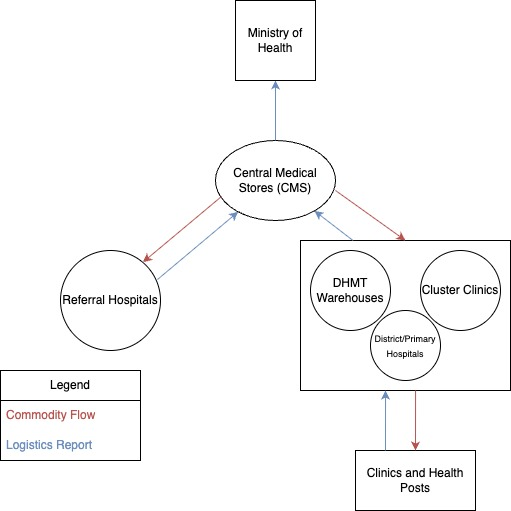
\includegraphics[width=0.5\textwidth]{DiagramofLogisticsBotswana (1) (1).jpg}
    \caption{Simplified overview of Botswana’s pharmaceutical distribution system, adapted from the \textit{Standard Operating Procedures Manual for the Logistics Management of Health Commodities in Botswana} (2019) and USAID GHSC-PSM (2021) \cite{ghsc2021botswana, botswanaSOP2019}.}
    \label{fig:health_flow}
\end{figure}

CMS is equipped with 8,999 pallet slots, guided forklifts, and the ePulse warehouse management system, but its utilization rate has reached 96\%, exceeding the recommended operational threshold of 90\% \cite{ghsc2021botswana}. This congestion slows order fulfillment and limits flexibility. DHMT warehouses often lack dedicated vehicles and rely on ambulances or ad hoc transport, while clinics and health posts use inconsistent paper or digital inventory systems. Many facilities have limited storage space, insufficient cold chain capacity, and no backup power or pest control, leading to frequent stock discrepancies and delays in disposing of expired products.  

The 2021 USAID Botswana Warehousing and Storage Assessment recommended revising the national distribution strategy, standardizing warehouse design, integrating inventory platforms, and expanding technical capacity \cite{ghsc2021botswana}. This thesis will build on these recommendations by developing a network optimization model that accounts for uncertainty in demand, storage, and vehicle availability. The model aims to focus on CMS and its downstream distribution to DHMT warehouses, clinics, and health posts, identifying bottlenecks and guide resource allocation for a more resilient and data-informed pharmaceutical supply chain.

\section{Literature Review}

Efficient antimicrobial distribution remains a critical challenge in regions with dispersed populations and limited healthcare capacity. Although prior work has optimized health supply chains under stochastic assumptions, few network models account for epidemiological feedback between intervention and disease spread. We aim to embed an SEIR constraint structure into an optimization formulation to dynamically allocate antimicrobials in response to evolving infection levels. The following section reviews key contributions in supply chain optimization under uncertainty, robust and adjustable robust optimization, antimicrobial resistance, and supply chain resilience.

\subsection{Supply Chain Optimization under Uncertainty}

Classical supply chain models such as the Economic Order Quantity (EOQ) minimize holding and ordering costs under constant demand and instantaneous replenishment \cite{harris13}. Although useful for simple systems, these formulations do not address perishability, capacity limits, or network constraints that are critical in health supply chains. Subsequent models incorporated uncertainty to better capture the variability inherent in real-world systems. Broadly, these models extend deterministic formulations by introducing uncertain parameters for demand, supply, or transportation times, allowing planners to evaluate system performance under multiple potential outcomes \cite{yu97}.

A general inventory balance constraint commonly used in multi-echelon systems is
\begin{equation}
I_{i,p,t+1} = I_{i,p,t} + \sum_{j \in \text{in}(i)} F_{j \to i, p, t} - \sum_{k \in \text{out}(i)} F_{i \to k, p, t} - D_{i,p,t},
\label{eq:perea}
\end{equation}
where $I$ is inventory, $F$ is flow between nodes, and $D$ is demand in location $i$ for product $p$ at time $t$ \cite{perea3}. This equation provides the structural basis for many supply chain formulations, linking upstream and downstream flows across time and space.

Although most applications have focused on cost minimization, health supply chains introduce additional considerations such as service-level targets and penalties for expirations or stockouts. These objectives reflect broader public health priorities rather than purely logistical efficiency. This motivates a closer examination of frameworks capable of capturing uncertainty without relying on full probabilistic information, such as robust and adjustable robust optimization methods discussed in the next section.

\subsection{Robust and Adjustable Robust Optimization in Inventory Problems}

Robust optimization provides a framework for decision making under uncertainty without requiring full probabilistic information. Instead of relying on expected values, robust formulations seek solutions that remain feasible for all realizations of uncertain parameters within a prescribed uncertainty set. The general framework introduced by \cite{bental} formalized this approach and demonstrated that tractable robust counterparts can be derived for large-scale linear programs through duality-based reformulations. Subsequent work by \cite{bertsim04} introduced the \textit{budgeted uncertainty set}, which limits the number or intensity of parameters that can simultaneously deviate to their worst-case values, thereby offering a tunable balance between conservatism and performance. This approach has proven particularly effective for applications in data-limited environments such as healthcare logistics, where full distributional information is rarely available.

Adjustable robust optimization (ARO) extends this framework by allowing certain decisions to adapt to realized uncertainty. Rather than solving for a single fixed decision, the model defines a decision policy that updates as new information becomes available. A common approach is to approximate adaptability through affine decision rules, which express decisions as linear functions of observed uncertainty realizations. As reviewed by \cite{yanikoglu2018aro}, this method enables tractable implementation of adaptive strategies in sequential production or inventory problems with uncertain demand. Such flexibility is particularly valuable in public health systems like Botswana’s, where new information on disease prevalence or medicine consumption can inform mid-horizon allocation updates.

\subsection{Modeling Drug Demand}
\label{2.3}

In the pharmacoepidemiology and health services literature, count outcomes such as prescription drug utilization, opioid related emergency department visits, or outpatient encounter frequencies typically exhibit substantial overdispersion, where the variance of the count variable exceeds its mean. This characteristic violates the equidispersion assumption of the Poisson model and motivates the use of more flexible specifications. For example, \cite{sec2017} employs a negative binomial regression to model opioid related emergency department visit counts adjusted for alternative measures of drug availability, illustrating that negative binomial models can accommodate the heterogeneity and dispersion that routinely arise in drug related event data. Their analysis highlights how underlying variability in exposure, case mix, and reporting practices can generate dispersion levels that exceed the capacity of a Poisson formulation.

A broader comparison of count data methods is provided by \cite{ab2022}, who evaluate Poisson, negative binomial, zero inflated and hurdle models for outpatient health services utilisation. Their results indicate that zero inflated models may offer improved fit when the data generating process includes a distinct source of excess zeros, such as structural non-utilisation at the individual level. Importantly, their discussion clarifies that the choice between negative binomial and zero inflated specifications depends on whether zeros arise from the same stochastic mechanism that generates positive counts or from a separate process. This distinction is central to model selection in applied health systems settings.

A recent review by \cite{rath2024} similarly emphasizes that drug utilization measures often violate Poisson equidispersion and identifies the negative binomial distribution as an appropriate specification in such settings. The review situates negative binomial models within the broader aims of pharmacological treatment evaluation, noting that accurate characterization of utilization patterns is essential for understanding treatment effectiveness, resource allocation and potential disparities in access. The discussion also underscores that variability in utilization arises from clinical, demographic and behavioral factors that naturally produce count distributions with higher variance than mean.

Taken together, these studies demonstrate that overdispersion is an inherent feature of drug related and health service count outcomes, and that negative binomial models provide a flexible and interpretable framework for addressing this feature. They further clarify that zero inflated approaches are warranted when a separate zero generating mechanism is present, which provides guidance for selecting an appropriate model in settings where structural zeros are absent. The zero-inflated structure identified in \cite{ab2022} arises from structural non-utilisation at the individual level, where a large subpopulation records no outpatient visits at all. Facility level drug stock data do not necessarily exhibit this mechanism, since all facilities participate in the supply chain and zeros may represent realized demand changes within the same stochastic process that generates positive counts.

\subsection{Antimicrobial Resistance and Externalities}

Traditional supply chain models rarely internalize the broader public health externalities associated with antimicrobial use. Delayed or incomplete treatment can accelerate the emergence of resistant pathogens, creating costs that extend beyond immediate stockouts or expirations \cite{lax13}. Foundational work by \cite{lax01} conceptualized antimicrobial resistance as an accumulating stock in a dynamic system, showing that myopic prescribing leads to socially suboptimal outcomes. Although these models focus on prescribing rather than logistics, the principle that short-term allocation decisions have long-term epidemiological consequences applies directly to supply chain planning.

Recent literature has attempted to capture these effects through health-based penalty terms or scenario weighting. Disability-Adjusted Life Years (DALYs), for instance, provide a metric for quantifying the social burden of delayed or incomplete access to essential medicines \cite{dar21}. Integrating DALY-based penalties into objective functions allows models to account for downstream health losses, though this approach requires caution due to limitations in DALY weighting across age and socioeconomic groups \cite{arne99}. Applying such metrics to Botswana’s centralized supply chain, albeit with some careful interpretation, could help align operational efficiency and demand fulfillment with a measure of public health impact.

\subsection{Supply Chain Resilience}

Beyond efficiency and cost-minimization, resilience, or the system's capacity to anticipate and recover from disruptions, is a key consideration in pharmaceutical logistics. \cite{tkr22} showed that pharmaceutical networks are particularly vulnerable to correlated shocks such as supplier failures, transport delays, and quality recalls, mainly due to the limited substitutability of essential medicines. Their reliability framework introduced probabilistic measures of expected shortages and recovery times, which can be adapted to the import-dependent network of Botswana by treating upstream nodes as suppliers and customs checkpoints rather than production sites.

Later work expanded the concept of resilience to include agility and sustainability. \cite{ivanov22} proposed the notion of viable supply chains that maintain continuity in prolonged or overlapping crises. Their approach highlights that robustness alone may not be enough to ensure adaptability once disruptions occur. In public health systems with rigid procurement cycles and limited transport capacity, this integration of resilience and agility is especially important.

In the context of medical supply chains, unique disruptions arise in the form of epidemics. \cite{govindan20} applied multi-objective optimization to allocate scarce medical resources under epidemic uncertainty, demonstrating that resilient strategies must balance efficiency and equity when demand surges occur simultaneously across regions. Therefore, improved data visibility and communication between CMS and district warehouses constitute a practical form of resilience, and equitable distribution should be an important consideration of any accurate predictive model for medical distribution. Further promise in the literature for the integration of epidemic-based constraints with supply chain networks are discussed in \ref{sec:twopointsix}.

\subsection{Embedding Epidemiological Feedback}
\label{sec:twopointsix}

Conventional supply chain reliability models typically assume that failures and recoveries occur independently in all locations. In public health systems, this assumption often breaks down because infectious disease dynamics create correlated and time-dependent demand shocks. Epidemics can synchronize demand surges across facilities, reduce workforce availability, and strain transport capacity simultaneously. To address this, several studies have integrated compartmental disease models with logistics and resource allocation frameworks.

\cite{bertsimas21} demonstrated how epidemiological forecasting can directly inform prescriptive decisions by embedding the dynamics of an SEIR-type disease within a data-driven optimization model in the context of the COVID-19 pandemic. Recent work by \cite{gpt23}  combines Bayesian inference with SEIR simulations to generate probabilistic demand trajectories, showing that uncertainty in disease spread can be incorporated into real-time decision systems. Earlier theoretical work by \cite{kd20} extended SEIR frameworks to include treatment-induced resistance, providing a tractable framework to properly link the extent of medical intervention to the evolution of resistant strains.

These models collectively illustrate the value of coupling epidemic evolution with supply allocation. By linking infection prevalence to demand, planners can anticipate future shortages, prioritize critical regions, and mitigate the secondary health effects of delayed treatment. For Botswana’s antimicrobial distribution network, embedding epidemiological feedback would enable the system to adapt to emerging AMR outbreaks by dynamically updating demand forecasts and optimizing deliveries in response to spatial and temporal changes in infection levels. Incorporating such feedback structures transforms the model from a static optimization problem into a responsive decision framework that reflects the interdependence between disease transmission and supply chain performance.

\subsection{Contributions and Gaps}

Although extensive research has examined supply chain optimization, perishability, and epidemic modeling, few studies integrate these dimensions into a unified framework for antimicrobial distribution. This thesis addresses three main gaps in the literature.

\begin{enumerate}

\item \textbf{Coupling Epidemic Dynamics with Supply Chain Decisions:} Most supply chain models assume exogenous demand, ignoring how disease transmission shapes real-time needs for medical resources. This thesis embeds epidemic dynamics directly into a network optimization framework, allowing infections and supply decisions to co-evolve and enabling the model to capture how distribution failures compound resistance emergence over time.

\item \textbf{Incorporating Demand Uncertainty into Pharmaceutical Allocation:} Existing health supply chain models rarely account for the overdispersed, non-stationary demand distributions that characterize antimicrobial need in resource-constrained settings. This thesis introduces a Medical Demand Estimator based on Negative Binomial regression and embeds it within an adjustable robust optimization framework, producing allocation policies that are robust to demand uncertainty without requiring full distributional knowledge.

\item \textbf{Adapting Reliability Metrics to Import-Based Health Systems:} Existing reliability models assume internal production networks, which do not reflect Botswana's import-based pharmaceutical system. This thesis adapts those methods to assess resilience across CMS and district-level distribution, accounting for disruptions in transport and supply across a national multi-echelon network.

\end{enumerate}

\section{Data Sources}

\subsection{Available and Acquired Data}

This study draws on several datasets obtained from the Botswana Ministry of Health, as well as former officials with the Central Medical Stores and at the African Comprehensive HIV/AIDS Partnership (ACHAP), an important partner in the implementation of this project.

\subsubsection{Botswana National Health Facility Data}

Facility-level data were obtained from the Botswana Health Facility Master List maintained by the Ministry of Health and Wellness. The dataset includes the geospatial coordinates, ownership, level of care, and district affiliations of all registered health facilities in the country. These data were used to identify public-sector facilities and to construct the network of delivery nodes for the optimization model \cite{mohw_facilitylist}.

The locations of district warehouses were approximated using the coordinates of each health district’s administrative capital, or, if possible, the district's primary hospital. This approach reflects an operational structure in which District Health Management Team (DHMT) warehouses are typically situated in district capitals or near the district's anchoring primary hospital, though the exact coordinates are not publicly available. These approximations were used to define the intermediate nodes linking the Central Medical Stores (CMS) to health facilities within each district \cite{mapiki2025}.

\subsubsection{Population and Facility Geocoding}
\label{popfacgeocoding}

Population data were obtained from Statistics Botswana's 2022 national census, which enumerates all recognized towns, villages, and localities along with their total resident populations. Because the public release of these data does not include spatial coordinates, each settlement name was geocoded to obtain latitude and longitude values. Initial coordinates were generated using the OpenStreetMap Nominatim API, combining settlement and district names in the query string (e.g., ``Letlhakane, Central 
District, Botswana'') to improve match precision and disambiguate duplicate place names \cite{nominatim}. To ensure complete spatial coverage and correct potential mismatches, the Nominatim results were subsequently validated and refined using the Google Maps Geocoding API, which returned coordinates with higher positional accuracy for a small subset of unlocated or low-confidence settlements. The combined dataset produced valid coordinates accounting for approximately 83\% of Botswana's total population.

The remaining 17\% of the population resided in settlements that could not be reliably geocoded using either API, predominantly small and remote rural localities lacking consistent place-name records. To avoid systematically excluding rural demand from the model, these settlements were assigned approximate spatial locations by drawing coordinates uniformly at random within rectangular regions approximating their respective district boundaries. The resulting locations were then matched to the nearest health facility using straight-line distance, ensuring that their associated populations contributed to facility-level demand estimates. While this approach introduces positional imprecision for affected settlements, it preserves the aggregate demand signal from rural areas and prevents the model from over-concentrating allocations toward better-documented urban facilities. Further discussed in Section \ref{botswananatadap}, this treatment becomes particularly consequential at national scale, where ungeocoded settlements are disproportionately rural and their demand is material to the spatial distribution of the allocation solution.

\subsubsection{Road-Network Distances and Spatial Linkage}
\label{3.1.4}

Health-facility coordinates were compiled from the Ministry of Health and Wellness master facility registry and augmented with warehouse locations. Service-delivery types were standardized into consistent categories (Health Post, Clinic, Clinic with Maternity, Primary Hospital, District Hospital, and Referral Hospital), with Clinics and Clinics with Maternity jointly treated as a single \textit{clinic-tier} level for access modeling. Facilities labeled as ``school clinic'' or ``prison clinic'' were excluded to restrict the analysis to civilian, publicly accessible sites.

Each populated census tract was linked to its closest health facilities using a $k$-d tree nearest-neighbor search implemented in Python’s \texttt{scipy.spatial.cKDTree} module. For every settlement–facility pair, the $k$-d tree identified the nearest facility by minimizing great-circle distance on the Earth's surface, providing an initial topological linkage between population demand points and service locations.

A national routing network was then constructed using the Open Source Routing Machine (OSRM) and the most recent OpenStreetMap (OSM) extract for Botswana obtained from Geofabrik \cite{geofabrik}. The OSRM backend was deployed locally in a Docker container to ensure reproducibility and full control over routing parameters \cite{osrm}. The compiled network, containing approximately 16.5 million nodes and 1.8 million edges, enabled detailed modeling of travel routes across paved, gravel, and unpaved roads.

To incorporate transport accessibility, each census tract was routed to its nearest Health Post, Clinic (including Maternity), and Primary Hospital using the locally hosted OSRM instance. The resulting origin–destination list provided road-network travel distances (in kilometers) and estimated travel times (in minutes) between census tracts and facilities. This hybrid $k$-d tree and OSRM framework yielded a tractable approximation of service catchments that integrates both spatial proximity and realistic network connectivity.

The final dataset excluded non-public facilities and retained 10,492 census tracts, each assigned to its closest health post, clinic, and primary hospital. This integrated approach was able to assign 282 of 328 health posts, 220 of 258 clinics, and 15 of 15 primary hospitals considered in the model. Unassigned health facilities will be handled on a case-by-case basis to their nearest census tract, and may have resulted from extremely dense population areas that assigned populations to other health facilities nearby. This spatial framework will form the basis for subsequent optimization of supply-chain logistics and facility-level resource allocation \cite{statsbotswana2022}.

Ethical approval to conduct this study was granted by the Health Research and Development Division (HRDD) of the Botswana Ministry of Health under reference number HPRD: 6/14/1, with an approval date of 11th February 2026 and an expiration date of 10th February 2027. The study was reviewed under an expedited process and determined to present minimal risk.

Data were subsequently obtained from the Central Medical Stores (CMS) under the study title \textit{Designing Robust Antimicrobial Supply Chains under Epidemiological Demand Uncertainty in Botswana}. The received dataset contains inventory and procurement records for 84 antimicrobial products 
as of 11th March 2026, spanning drug classes 200 through 600 and including a small number of products flagged for removal (RFD). For each product, the dataset provides the product code, description, unit of issue, VEN classification (Vital, Essential, or Non-essential), unit price, current stock levels at CMS, and average monthly consumption estimates for both 2025--26 and 2026--27, along with corresponding months of stock on hand. The approved records in partnership with CMS provide the empirical basis for unit procurement costs (in Botswana Pula, BWP) and baseline stock initialization in the national allocation model, and represent a great addition to the otherwise simulation-based components of this work. All data are aggregated and non-personal, in full compliance with HRDC ethical standards.

To initialize facility-level inventory states for the national model trials in Section~\ref{cmsresults}, aggregate CMS stock levels are disaggregated across facilities using catchment population proportions. Specifically, the current stock of each antimicrobial product at CMS is allocated to each facility in proportion to its share of the total catchment population served by the network, as determined by the geocoding and nearest-facility assignment procedure described in Section~\ref{popfacgeocoding}. This approach provides a principled baseline initialization that reflects the relative scale of demand across facilities, while remaining agnostic to the historical distribution decisions of the CMS.

\section{Methods}

\subsection{Network Construction}
\label{4.1}

631 facilities were matched to the Botswana Ministry of Health's master facility list. 22 district-level warehouses were identified as distribution hubs, including 3 (Northeast, Tutume, and Francistown) that share the same physical warehouse location in Francistown. The resulting dataset distinguishes between warehouses and service delivery points and forms the basis for the national distribution graph $G = (N, A)$, where nodes $N$ represent health facilities and arcs $A$ represent feasible delivery routes.

Pairwise road distances were computed using OSRM's \texttt{/table} API endpoint, which returns shortest-path distances between all origin--destination pairs \cite{osrm}. The resulting distance matrix is 
$631 \times 631$, representing 398{,}161 unique origin--destination pairs across the national network. The final network comprises 22 warehouses, 3 national referral hospitals, 10 district hospitals, 15 primary hospitals, 258 clinics, and 328 health posts, as seen in Figure~\ref{fig:faccts}.\footnote{Note that there are more clinics and health posts than described in Section~\ref{3.1.4}, which eliminated school or prison-based facilities not accessed by the general public.} Each facility was labeled by service-delivery category to enable aggregation and stratified analysis.

\begin{figure}
    \centering
    \begin{minipage}[b]{0.48\linewidth}
        \centering
        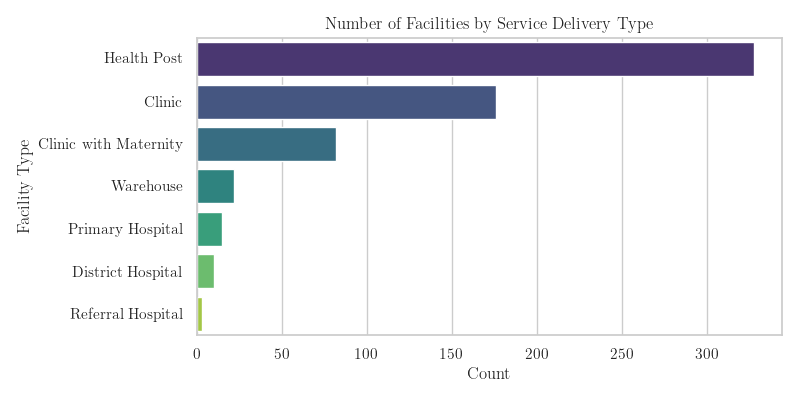
\includegraphics[width=\linewidth]{facility_type_counts.png}
        \caption{Facility type counts included in the distance matrix.}
        \label{fig:faccts}
    \end{minipage}
    \hfill
    \begin{minipage}[b]{0.48\linewidth}
        \centering
        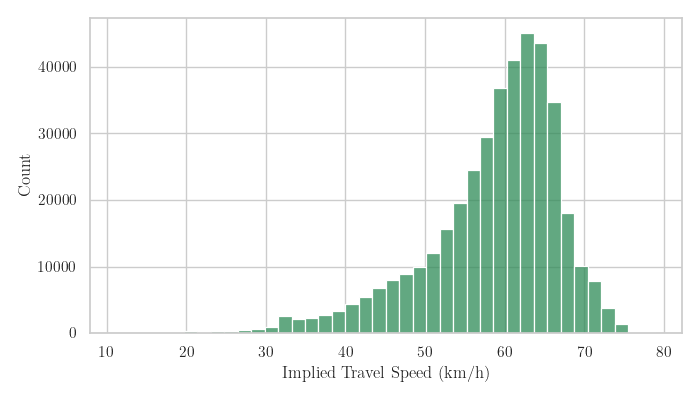
\includegraphics[width=\linewidth]{speed_distribution.png}
        \caption{Implied speeds derived from OSRM routes, used to validate 
        routing realism. Speeds are computed as distance divided by travel 
        duration across all origin--destination pairs.}
        \label{fig:speeddist}
    \end{minipage}
\end{figure}

To validate routing performance, OSRM-generated travel times were converted into implied speeds by dividing road distance by travel duration for all origin--destination pairs, and multiplying by 1.2 to account for road uncertainty and inclement weather conditions. As shown in Figure~\ref{fig:speeddist}, the 
resulting speed distribution has a median of approximately 58~km/h, with most within-district trips falling between 40--70~km/h and inter-district routes exhibiting greater variability due to unpaved segments and longer rural distances. This distribution provides reassurance that OSRM captures 
realistic travel dynamics across Botswana's mixed road network.

\subsection{Notation and Variable Definitions}
\label{4.2}

To construct the first-stage optimization model, we begin by defining our sets, indices, parameters and decision variables.

\subsubsection{Model Structure and Notation}
\label{4.2.1}

We model the antimicrobial distribution network as a directed graph \(G = (N, A)\), where:

\begin{itemize}
  \item $N$: set of nodes representing public-sector health facilities (e.g., the Central Medical Stores, DHMT warehouses, hospitals, clinics, and health posts), indexed by \(n \in \{0, 1, \dots, F-1\}\), with \(F\) representing the total number of facilities.
  \item $K$: set of antimicrobial product types, indexed by \(k \in \{0, 1, \dots, K-1\}\)
  \item $A \subseteq N \times N$: set of directed arcs \((i,j)\) representing feasible transportation routes between facilities; flows are permitted only downstream from CMS to DHMT warehouses and lower-level facilities
  \item $t = \{0, 1, \dots, T\}$: set of discrete time periods representing decision epochs (each typically corresponding to two weeks)
\end{itemize}

\subsubsection{Parameters}
\label{4.2.2}

The following parameters describe the physical and operational characteristics of the network.  
Unless otherwise stated, all parameters are assumed to be known at the beginning of each planning period.

\begin{itemize}
  \item $\text{Dist}_{ij}$: road-network distance between nodes \(i\) and \(j\), computed using OSRM outputs (in kilometers or meters) [this is also replaceable with $\text{Dur}_{ij}$, or the estimated travel duration in hours]
  \item $v$: per-unit transportation cost, proportional to either distance or travel time
  \item $\Delta_{n,k}$: penalty cost per unit of unmet demand for drug \(k\) at node \(n\)
  \item $h$: per-unit per-period holding cost for inventory carried over to the next epoch
  \item $D_{n,k}^{(t)}$: realized demand for drug \(k\) at node \(n\) in the current period
  \item $s_n$: maximum storage capacity at facility \(n\)
  \item $\text{cap}$: vehicle or route capacity, denoting the maximum shipment quantity per trip
  \item $M$: large constant used in binary activation constraints to link route-use variables and flows
\end{itemize}

\subsubsection{Decision Variables}
\label{4.2.3}

Decision variables represent shipment quantities, inventory levels, unmet demand, and route activations:

\begin{itemize}
  \item $F_{(i,j),k}^{(t)}$: quantity of drug \(k\) shipped from facility \(i\) to facility \(j\) at the beginning of the current period
  \item $I^{(t)}_{n,k}$: inventory of drug \(k\) at node \(n\) at the beginning of the current period
  \item $I^{(t+1)}_{n,k}$: inventory of drug \(k\) at node \(n\) at the end of the current period
  \item $U_{n,k}^{(t)}$: unmet demand for drug \(k\) at node \(n\) realized during the current period
  \item $\lambda_{(i,j)}^{(t)}$: number of vehicle trips (or route activations) from \(i\) to \(j\) at the beginning of the current period
  \item $y_{(i,j)}^{(t)}$: binary variable equal to 1 if route \((i,j)\) is active for the current period, and 0 otherwise
  \item $q_k^{(t)}$: quantity of antimicrobial class $k$ procured at the CMS at the beginning of period $t$
\end{itemize}

\subsubsection{Uncertainty Parameters (Robust Extension)}
\label{4.2.4}

To model uncertainty in demand, we introduce the following quantities:

\begin{itemize}
  \item $\bar{D}_{n,k}^{(t)}$: nominal (expected) demand for drug \(k\) at facility \(n\) in the current period
  \item $\sigma_{n,k}^{(t)}$: maximum deviation of demand from its nominal value in the current period
  \item $\xi_{n,k}^{(t)}$: realized demand deviation, treated as an uncertain variable
  \item $\Gamma$: uncertainty budget limiting the number of facilities that can simultaneously experience worst-case demand shocks
  \item $z_{n,k}^{(t)}$: auxiliary variable used in the reformulation of the uncertainty set when deriving the robust counterpart
\end{itemize}

\subsection{Baseline Optimization Model}
\label{4.3}

The deterministic baseline model minimizes total transportation, shortage, holding, and procurement costs across the national distribution network. Demand is treated as known and equal to its nominal value. The formulation is given in Equations (2) through (12):

\begin{equation}
\min_{F^{(t)}, \lambda^{(t)}, y^{(t)}, U^{(t)}, I^{(t+1)}, q^{(t)}} 
v \sum_{(i,j)\in A} \text{Dist}_{ij}\lambda_{(i,j)}^{(t)} +
\sum_{n\in N}\sum_{k\in K}
\left(\Delta_{n,k}U_{n,k}^{(t)} + h I^{(t+1)}_{n,k}\right)
+ \sum_{k\in K} c_k^{\text{proc}} q_k^{(t)}
\end{equation}

subject to the following constraints:

\begin{align}
I^{(t+1)}_{n,k} &= I^{(t)}_{n,k} 
+ \sum_{j:(j,n)\in A} F_{(j,n),k}^{(t)} 
- \sum_{m:(n,m)\in A} F_{(n,m),k}^{(t)} 
- D_{n,k}^{(t)} 
+ U_{n,k}^{(t)}, 
&& \forall n \in N \setminus \{0\},\; k \in K, \\
I^{(t+1)}_{0,k} &= I^{(t)}_{0,k} 
+ q_k^{(t)}
- \sum_{m:(0,m)\in A} F_{(0,m),k}^{(t)}, 
&& \forall k \in K, \\
\sum_{m:(n,m)\in A} F_{(n,m),k}^{(t)}
&\le
I_{n,k}^{(t)}
+
\sum_{j:(j,n)\in A} F_{(j,n),k}^{(t)}
+
\mathbf{1}_{\{n=\mathrm{CMS}\}}\, q_k^{(t)},
&& \forall n \in N,\; k \in K, \\
\sum_{k\in K} F_{(i,j),k}^{(t)} 
&\le \text{cap} \cdot \lambda_{(i,j)}^{(t)}, 
&& \forall (i,j) \in A, \\
\lambda_{(i,j)}^{(t)} 
&\le M \, y_{(i,j)}^{(t)}, 
\quad y_{(i,j)}^{(t)} \in \{0,1\}, 
&& \forall (i,j) \in A, \\
\sum_{k\in K} I^{(t+1)}_{n,k} 
&\le s_n, 
&& \forall n \in N, \\
F_{(i,j),k}^{(t)} &\ge 0, 
&& \forall (i,j)\in A, k\in K, \\
I^{(t+1)}_{n,k} &\ge 0, \quad 
U_{n,k}^{(t)} \ge 0, 
&& \forall n \in N, k \in K, \\
q_k^{(t)} &\ge 0, 
&& \forall k \in K, \\
\lambda_{(i,j)}^{(t)} &\in \mathbb{Z}_+.
\end{align}

All shipment decisions $F_{(i,j),k}^{(t)}$ and routing decisions are made at the beginning of period $t$, given inventory levels $I^{(t)}_{n,k}$. Demand $D_{n,k}^{(t)}$ is realized during the period, after which unmet demand $U_{n,k}^{(t)}$ and end-of-period inventory $I^{(t+1)}_{n,k}$ are determined. In the deterministic baseline model, demand is assumed to equal its nominal value, i.e., $D_{n,k}^{(t)} = \bar{D}_{n,k}^{(t)}$.

The model ensures inventory balance, enforces capacity and binary activation constraints, and maintains non-negativity across all decision variables. It provides a tractable benchmark for evaluating total cost and flow feasibility under nominal demand conditions.

\subsection{Extension to Robust Optimization}
\label{4.4}

To incorporate demand uncertainty, we follow the robust optimization paradigm introduced by \cite{bental} and the adjustable extensions reviewed by \cite{yanikoglu2018aro}. Demand for each antimicrobial class \(k\) at node \(n\) is modeled as
\begin{equation}
D_{n,k}^{(t)} = \bar{D}_{n,k}^{(t)} + \xi_{n,k}^{(t)},
\end{equation}
where \(\bar{D}_{n,k}^{(t)}\) is nominal demand and \(\xi_{n,k}^{(t)}\) represents an uncertain deviation.

Uncertainty is modeled using a budgeted polyhedral uncertainty set for each drug class \(k\):
\begin{equation}
\mathcal{U}_D^{(k)} =
\left\{
\xi :
|\xi_{n,k}^{(t)}| \le \sigma_{n,k}^{(t)}, \;
\sum_{n \in N} \frac{|\xi_{n,k}^{(t)}|}{\sigma_{n,k}^{(t)}} \le \Gamma
\right\}.
\end{equation}
Here, \(\sigma_{n,k}^{(t)}\) denotes the maximum deviation magnitude for node \(n\) and drug class \(k\), while \(\Gamma\) controls the total number of nodes that may simultaneously experience large deviations.

Following \cite{bertsim04} for tractable dualization, we introduce nonnegative deviation variables
\begin{equation}
\xi_{n,k}^{(t)} = \sigma_{n,k}^{(t)}\left(z_{n,k}^{+(t)} - z_{n,k}^{-(t)}\right),
\end{equation}
with
\begin{equation}
0 \le z_{n,k}^{+(t)} \le 1, \quad 0 \le z_{n,k}^{-(t)} \le 1.
\end{equation}

The uncertainty set can then be written equivalently as
\begin{equation}
\mathcal{Z}^{(k)} =
\left\{
(z^+,z^-)\in[0,1] :
\sum_{n \in N} \left(z_{n,k}^{+(t)} + z_{n,k}^{-(t)}\right) \le \Gamma
\right\}.
\end{equation}

The deterministic inventory balance requires
\begin{equation}
I^{(t+1)}_{n,k} =
I^{(t)}_{n,k}
+ \sum_{j:(j,n)\in A} F^{(t)}_{(j,n),k}
- \sum_{m:(n,m)\in A} F^{(t)}_{(n,m),k}
- D^{(t)}_{n,k}
+ U^{(t)}_{n,k}.
\end{equation}

Under uncertain demand, the planner must ensure that the inventory balance remains feasible for all realizations \(\xi^{(t)} \in \mathcal{U}_D^{(k)}\). Substituting \(D^{(t)}_{n,k} = \bar{D}^{(t)}_{n,k} + \xi^{(t)}_{n,k}\), the robust constraint becomes
\begin{equation}
I^{(t+1)}_{n,k} =
I^{(t)}_{n,k}
+ \sum_{j:(j,n)\in A} F^{(t)}_{(j,n),k}
- \sum_{m:(n,m)\in A} F^{(t)}_{(n,m),k}
- \bar{D}^{(t)}_{n,k}
- \xi^{(t)}_{n,k}
+ U^{(t)}_{n,k},
\quad \forall \xi^{(t)} \in \mathcal{U}_D^{(k)}.
\end{equation}
This expression is used to derive the robust feasibility constraints; however, because $\xi_{n,k}^{(t)}$ appears in an equality, we do not enforce this relation directly for all $\xi^{(t)} \in \mathcal{U}_D^{(k)}$, and our method for avoiding this is described in Section \ref{5.5}.

Relative to the deterministic model, the uncertainty term \(\xi_{n,k}^{(t)}\) can either increase or decrease effective demand. The budget constraint \(\Gamma\) limits the number of simultaneous large deviations, providing a tunable trade-off between robustness and efficiency.

\subsection{Affine Decision Rules}
\label{5.5}

While the static robust formulation protects against worst-case demand realizations, it does so conservatively by fixing shipment quantities entirely in advance, leaving no room to exploit demand information as it is revealed. A key modelling choice in the ARO-ADR formulation is how the adaptive shipment policy is parameterized. At the start of each period the planner commits simultaneously to a nominal shipment plan $\bar{F}_{(u,v),k}^{(t)}$ and a set of response coefficients $\alpha_{(u,v),k}^{(t)}$, both optimized before any demand deviation $\xi_{n,k}^{(t)}$ is observed. Once demand is realized, the actual shipment adjusts linearly according to the affine rule defined below. There is therefore no look-ahead: the optimizer finds the best linear response policy given only the structure of the uncertainty set, committing to both the plan and its recourse before uncertainty is revealed.

\subsubsection{Reformulated Problem with Affine Decision Rules}

Because the inventory balance contains the uncertain quantity $\xi_{n,k}^{(t)}$ within an equality constraint, it cannot be enforced directly for all realizations of the uncertainty. Instead, we replace it
with a robust feasibility condition before stating the full problem. Substituting the affine decision rule
$F_{(u,v),k}^{(t)}(\xi^{(t)}) = \bar F_{(u,v),k}^{(t)} + \alpha_{(u,v),k}^{(t)}\xi_{v,k}^{(t)}$ into the inventory balance and collecting uncertain terms, the uncertain component on the left-hand side represents the net effect of demand deviations on inventory through both incoming and outgoing adaptive shipments. The right-hand side captures the slack available in the nominal inventory balance after accounting for planned flows, procurement, and the unmet demand variable $U_{n,k}^{(t)}$, which absorbs any residual shortfall under nominal demand. Robust feasibility then requires that this worst-case uncertain perturbation does not exceed the available slack:
\begin{align}
\left(
\sum_{j:(j,n)\in A} \alpha_{(j,n),k}^{(t)} - 1
\right)\xi_{n,k}^{(t)}
-
\sum_{r:(n,r)\in A} \alpha_{(n,r),k}^{(t)} \xi_{r,k}^{(t)}
\le\;&
I_{n,k}^{(t+1)}
-
I_{n,k}^{(t)}
-
\sum_{j:(j,n)\in A} \bar F_{(j,n),k}^{(t)}
+
\sum_{m:(n,m)\in A} \bar F_{(n,m),k}^{(t)}
\notag\\
&-
\mathbf{1}_{\{n=\mathrm{CMS}\}} q_k^{(t)}
+
\bar D_{n,k}^{(t)}
-
U_{n,k}^{(t)},
\notag\\
&\qquad \forall \xi^{(t)}\in\mathcal{U}^{(t)},\ \forall n \in N,\ k \in K.
\label{eq:robust_inventory}
\end{align}
This converts the problematic equality into a tractable robust inequality, which we incorporate directly into the problem formulation below. The robust counterpart with affine decision rules is then:
\begin{align}
\min_{\substack{\bar F^{(t)},\,\alpha^{(t)},\,\lambda^{(t)}\\y^{(t)}, 
U^{(t)},\,I^{(t+1)}\\q^{(t)}}}
\quad
\max_{\xi^{(t)}\in\mathcal U^{(t)}}
\quad &
v \sum_{(i,j)\in A} \mathrm{Dist}_{ij}\lambda_{(i,j)}^{(t)}
+
\sum_{k\in K} c_k^{\mathrm{proc}} q_k^{(t)}
+
\sum_{n\in N}\sum_{k\in K}
\left(
\Delta_{n,k}U_{n,k}^{(t)} + h I_{n,k}^{(t+1)}
\right)
\\
\text{s.t.}\quad
&
F_{(u,v),k}^{(t)}(\xi^{(t)})=
\bar F_{(u,v),k}^{(t)}
+
\alpha_{(u,v),k}^{(t)}\,\xi_{v,k}^{(t)},
\qquad \forall (u,v)\in A,\ k\in K,
\\
&
\left(
\sum_{j:(j,n)\in A} \alpha_{(j,n),k}^{(t)} - 1
\right)\xi_{n,k}^{(t)}
-
\sum_{r:(n,r)\in A} \alpha_{(n,r),k}^{(t)} \xi_{r,k}^{(t)}
\notag\\
&\quad\le
I_{n,k}^{(t+1)}
-
I_{n,k}^{(t)}
-
\sum_{j:(j,n)\in A} \bar F_{(j,n),k}^{(t)}
+
\sum_{m:(n,m)\in A} \bar F_{(n,m),k}^{(t)}
\notag\\
&\quad\phantom{\le}
-
\mathbf{1}_{\{n=\mathrm{CMS}\}} q_k^{(t)}
+
\bar D_{n,k}^{(t)}
-
U_{n,k}^{(t)},
\notag\\
&\quad\phantom{\le}
\forall \xi^{(t)}\in\mathcal{U}^{(t)},\ 
\forall n\in N,\ k\in K,
\\
&
\sum_{m:(n,m)\in A} F_{(n,m),k}^{(t)}(\xi^{(t)})
\le\;
I_{n,k}^{(t)}
+
\sum_{j:(j,n)\in A} F_{(j,n),k}^{(t)}(\xi^{(t)})
+
\mathbf{1}_{\{n=\mathrm{CMS}\}}\, q_k^{(t)},
\notag\\
&\qquad \forall n\in N,\ k\in K,
\\
&
\sum_{k\in K} F_{(i,j),k}^{(t)}(\xi^{(t)})
\le \mathrm{cap}\cdot \lambda_{(i,j)}^{(t)},
\qquad \forall (i,j)\in A,
\\
&
\lambda_{(i,j)}^{(t)} \le M\, y_{(i,j)}^{(t)},
\qquad \forall (i,j)\in A,
\\
&
y_{(i,j)}^{(t)} \in \{0,1\},
\qquad \forall (i,j)\in A,
\\
&
\sum_{k\in K} I_{n,k}^{(t+1)} \le s_n,
\qquad \forall n\in N,
\\
&
F_{(i,j),k}^{(t)}(\xi^{(t)}) \ge 0,
\qquad \forall (i,j)\in A,\ k\in K,
\\
&
I_{n,k}^{(t+1)} \ge 0,\quad U_{n,k}^{(t)} \ge 0,
\qquad \forall n\in N,\ k\in K,
\\
&
\lambda_{(i,j)}^{(t)} \in \mathbb{Z}_+,
\qquad \forall (i,j)\in A,
\\
&
q_k^{(t)} \ge 0,
\qquad \forall k\in K.
\end{align}
The details on dualization to yield a tractable single-level formulation are explained in Section~\ref{dual} and Appendix~\ref{app:dualization}.

\subsubsection{Dualization}
\label{dual}

To obtain a tractable single-level formulation, we dualize the inner maximization induced by demand uncertainty under the affine decision rule
\begin{align}
F_{(u,v),k}^{(t)}(\xi^{(t)})
=
\bar F_{(u,v),k}^{(t)}
+
\alpha_{(u,v),k}^{(t)} \xi_{v,k}^{(t)}.
\end{align}

Using the Bertsimas--Sim representation of the uncertainty set and standard linear programming duality, each robust constraint can be replaced by a finite collection of linear constraints. Thus, to handle inventory feasibility, shipment availability, and arc capacity,  we introduce the nonnegative dual variables $\theta_{n,k}^{(t)}$ and $\pi^{\pm}_{n,k,r}{}^{(t)}$ for the inventory constraints, $\tilde{\theta}_{n,k}^{(t)}$ and $\tilde{\pi}^{\pm}_{n,k,r}{}^{(t)}$ for the shipment availability constraints, and $\eta_{(i,j)}^{(t)}$ and $\rho^{\pm}_{(i,j),k}{}^{(t)}$ for the arc capacity constraints. The full derivation is provided in Appendix~\ref{app:dualization}.

\vspace{0.5em}

\textit{Inventory feasibility.} For each \(n \in N\), \(k \in K\),
\begin{align}
\Gamma \theta_{n,k}^{(t)}
+
\sum_{r \in N}
\left(
\pi^+_{n,k,r}{}^{(t)} + \pi^-_{n,k,r}{}^{(t)}
\right)
\le\;&
I_{n,k}^{(t+1)}
-
I_{n,k}^{(t)}
\notag\\
&-
\sum_{j:(j,n)\in A} \bar F_{(j,n),k}^{(t)}
+
\sum_{m:(n,m)\in A} \bar F_{(n,m),k}^{(t)}
\notag\\
&-
\mathbf{1}_{\{n=\mathrm{CMS}\}} q_k^{(t)}
+
\bar D_{n,k}^{(t)}
-
U_{n,k}^{(t)},
\end{align}
with
\begin{align}
\theta_{n,k}^{(t)} + \pi^+_{n,k,n}{}^{(t)}
&\ge
\left(
\sum_{j:(j,n)\in A} \alpha_{(j,n),k}^{(t)} - 1
\right)\sigma_{n,k}^{(t)}, \\
\theta_{n,k}^{(t)} + \pi^-_{n,k,n}{}^{(t)}
&\ge
-\left(
\sum_{j:(j,n)\in A} \alpha_{(j,n),k}^{(t)} - 1
\right)\sigma_{n,k}^{(t)}, \\
\theta_{n,k}^{(t)} + \pi^+_{n,k,r}{}^{(t)}
&\ge
-\sum_{m:(n,m)\in A} \alpha_{(n,m),k}^{(t)} \sigma_{r,k}^{(t)},
\quad \forall r:(n,r)\in A, \\
\theta_{n,k}^{(t)} + \pi^-_{n,k,r}{}^{(t)}
&\ge
\sum_{m:(n,m)\in A} \alpha_{(n,m),k}^{(t)} \sigma_{r,k}^{(t)},
\quad \forall r:(n,r)\in A.
\end{align}

\vspace{0.5em}

\textit{Shipment availability.} For each \(n \in N\), \(k \in K\),
\begin{align}
\Gamma \tilde{\theta}_{n,k}^{(t)}
+
\sum_{r \in N}
\left(
\tilde{\pi}^+_{n,k,r}{}^{(t)} + \tilde{\pi}^-_{n,k,r}{}^{(t)}
\right)
\le\;&
I_{n,k}^{(t)}
+
\sum_{j:(j,n)\in A} \bar F_{(j,n),k}^{(t)}
\notag\\
&+
\mathbf{1}_{\{n=\mathrm{CMS}\}} q_k^{(t)}
-
\sum_{m:(n,m)\in A} \bar F_{(n,m),k}^{(t)},
\end{align}
with
\begin{align}
\tilde{\theta}_{n,k}^{(t)} + \tilde{\pi}^+_{n,k,n}{}^{(t)}
&\ge
-\sum_{j:(j,n)\in A} \alpha_{(j,n),k}^{(t)} \sigma_{n,k}^{(t)}, \\
\tilde{\theta}_{n,k}^{(t)} + \tilde{\pi}^-_{n,k,n}{}^{(t)}
&\ge
\sum_{j:(j,n)\in A} \alpha_{(j,n),k}^{(t)} \sigma_{n,k}^{(t)}, \\
\tilde{\theta}_{n,k}^{(t)} + \tilde{\pi}^+_{n,k,r}{}^{(t)}
&\ge
\sum_{m:(n,m)\in A} \alpha_{(n,m),k}^{(t)} \sigma_{r,k}^{(t)},
\quad \forall r:(n,r)\in A, \\
\tilde{\theta}_{n,k}^{(t)} + \tilde{\pi}^-_{n,k,r}{}^{(t)}
&\ge
-\sum_{m:(n,m)\in A} \alpha_{(n,m),k}^{(t)} \sigma_{r,k}^{(t)},
\quad \forall r:(n,r)\in A.
\end{align}

\vspace{0.5em}

\textit{Arc capacity.} For each \((i,j) \in A\),
\begin{align}
\Gamma \eta_{(i,j)}^{(t)}
+
\sum_{k \in K}
\left(
\rho^+_{(i,j),k}{}^{(t)} + \rho^-_{(i,j),k}{}^{(t)}
\right)
\le\;&
\mathrm{cap}\cdot \lambda_{(i,j)}^{(t)}
-
\sum_{k\in K} \bar F_{(i,j),k}^{(t)},
\end{align}
with
\begin{align}
\eta_{(i,j)}^{(t)} + \rho^+_{(i,j),k}{}^{(t)}
&\ge
\alpha_{(i,j),k}^{(t)} \sigma_{j,k}^{(t)}, \\
\eta_{(i,j)}^{(t)} + \rho^-_{(i,j),k}{}^{(t)}
&\ge
-\alpha_{(i,j),k}^{(t)} \sigma_{j,k}^{(t)}.
\end{align}

\subsection{Medical Demand Estimator (MDE)}
\label{4.5}

A central challenge in forecasting antimicrobial requirements in Botswana is the absence of comprehensive, high-frequency patient-level clinical records. Available data consist of region-level demographic tabulations and a national point-prevalence survey (PPS) of inpatient antimicrobial use. The survey provides patient-level records from which we recover empirical marginal distributions (age by infection category, hospital tier by antimicrobial class, and HIV status by class); however, patient identifiers are not globally unique across sites, so the full patient-level joint distribution of characteristics, diagnoses, and treatment choices remains only partially identified. This motivates the calibrated synthetic reconstruction developed below, which reproduces the reliably observed marginals while smoothing the sparsely observed joint.

To construct a demand model compatible with these data constraints, we introduce a parametric estimator of guideline-appropriate antimicrobial need based on Negative Binomial regression and calibrated synthetic microdata. This section formalizes the statistical framework underlying the Medical Demand Estimator (MDE), specifies the assumptions required for identification, and establishes its large-sample consistency.

\newtheorem{assumption}{Assumption}
\newtheorem{definition}{Definition}
\newtheorem{remark}{Remark}
\newtheorem{theorem}{Theorem}
\newtheorem{lemma}{Lemma}

\begin{assumption}[Latent Clinical Demand]
\label{assump:dtrue}
For each region $r$ and age group $a$, let $N_{r,a}$ denote the number of admissions. Let $\mu_{r,a}$ denote the true incidence rate of clinically indicated infections requiring antimicrobial treatment, and let $\delta_a$ denote the guideline-recommended total dose for age group $a$ (for the purposes of simplifying the simulation, we treat this as one shipment unit of the drug). The true antimicrobial demand for region $r$ is
\[
D_r^{*}
=
\sum_a N_{r,a}\mu_{r,a}\delta_a.
\]
\end{assumption}

\begin{assumption}[Incidence Sampling Model]
\label{assump:nb}
For each region $r$ and age group $a$, let $Y_{r,a,t}$ denote the number of clinically indicated antimicrobial-treatment cases observed in survey unit $t$ of a point-prevalence survey (PPS). We observe $n$ independent realizations
\[
Y_{r,a,1},\dots,Y_{r,a,n}
\overset{\mathrm{i.i.d.}}{\sim}
\mathrm{NegBin}(\mu_{r,a},\kappa),
\]
where $\mu_{r,a}$ is the mean incidence for region $r$ and age group $a$, and $\kappa>0$ is a finite overdispersion parameter.
\end{assumption}

\begin{assumption}[NB--GLM Mean Specification]
\label{assump:glm}
The conditional mean satisfies the log-linear specification
\[
\mathbb{E}[Y_{r,a,t}\mid X_{r,a}]
=
\mu_{r,a}
=
\exp(X_{r,a}^{\top}\beta^{*}),
\]
where $X_{r,a}$ is a vector of observed covariates and $\beta^{*}$ is the true parameter vector.
\end{assumption}

The overdispersion parameter $\kappa$ is estimated jointly with the regression coefficients of the Negative Binomial generalized linear model by maximum likelihood. Under the NB2 parameterization, the variance satisfies
\[
\mathrm{Var}(Y_{r,a}) = \mu_{r,a} + \frac{\mu_{r,a}^2}{\kappa}.
\]
The fitted value $\hat{\kappa}$ characterizes the overdispersion of the reconstructed counts. Because $\hat{\kappa}$ is obtained from calibrated synthetic microdata rather than a repeated longitudinal sample, we do not treat it as a point estimate of the true demand dispersion. Instead, the simulation of stochastic antimicrobial demand treats $\kappa$ as a sensitivity parameter, swept over a range (e.g.\ $\kappa \in \{2, 10, 25\}$) that brackets the empirical per-patient overdispersion measured directly from the survey counts ($\hat{\kappa}\approx 3.7$ by method of moments).

In the baseline MDE, the covariate vector \(X_{r,a}\) contains observed predictors available from demographic tabulations and PPS summaries. These include region indicators, age-group indicators, facility or hospital-type indicators where applicable, infection-category indicators, patient comorbidity indicators (notably HIV status, given its prominence in the Botswana inpatient population), and interaction terms used when supported by the data. Thus \(X_{r,a}\) is not patient-level clinical history, but rather the collection of observed region-, age-, and facility-level features used to predict mean antimicrobial demand.

\begin{assumption}[Regularity Conditions]
\label{assump:regularity}
The parameter $\beta^{*}$ lies in the interior of a compact parameter space $\Theta\subset\mathbb{R}^{d}$. The likelihood is correctly specified, identifiable, and twice continuously differentiable, ensuring consistency of the MLE.
\end{assumption}

\begin{definition}[Medical Demand Estimator]
\label{def:mde}
Let $\hat\beta_n$ denote the NB--GLM maximum likelihood estimator. Define
\[
\hat\mu_{r,a}=\exp(X_{r,a}^{\top}\hat\beta_n).
\]
The Medical Demand Estimator for region $r$ is
\[
\hat D_r
=
\sum_a N_{r,a}\delta_a\hat\mu_{r,a}.
\]
\end{definition}

\begin{remark}[Model Choice]
Observed incidence counts exhibit substantial overdispersion due to heterogeneity in exposure, access to care, and clustering of infections. The Negative Binomial model provides a flexible and empirically validated framework for such data in epidemiological and pharmacological settings. These assumptions are further discussed in Section~\ref{2.3}.
\end{remark}

\begin{lemma}[Smoothness of the Demand Map]
\label{lem:smooth}
Define
\[
g(\beta)
=
\sum_a N_{r,a}\delta_a\exp(X_{r,a}^{\top}\beta).
\]
Then $g$ is continuous and twice continuously differentiable. Moreover, $g$ is Lipschitz on compact subsets of $\mathbb{R}^{d}$.
\end{lemma}

\begin{proof}
See Appendix~\ref{B.1}.
\end{proof}

\begin{theorem}[Consistency of the MDE]
\label{thm:nbglm_consistency}
Under Assumptions \ref{assump:dtrue}--\ref{assump:regularity},
\[
\hat D_r \xrightarrow{p} D_r^{*}
\qquad \text{as } n\to\infty.
\]
\end{theorem}

\begin{proof}
See Appendix~\ref{B.2}.
\end{proof}

\begin{assumption}[Synthetic Microdata Construction]
\label{assump:synthetic}
The PPS reports only aggregate prescription counts $\{C_i\}_{i=1}^{I}$ and marginal distributions of patient characteristics. Patient-level class assignments are unobserved.

We construct a synthetic dataset on the Cartesian product
\[
\mathcal{J}=\{1,\dots,P\}\times\{1,\dots,I\},
\]
and assign outcomes $Y_{j,i}$ such that the resulting data reproduce all observed marginal distributions.
\end{assumption}

The available data do not provide fully linked patient-level prescription records, but only aggregate or partially linked tabulations across key
dimensions such as antimicrobial class, age group, hospital type, and infection category. Consequently, the joint distribution of antimicrobial
requirements across classes at the individual patient level is not directly observable. In particular, while co-prescription patterns and clinical
correlations across antimicrobial classes are likely, they cannot be explicitly measured from the data. This raises the question of whether an aggregate demand model constructed from such incomplete information can still be theoretically justified. The following result addresses this issue by showing that, under independence across patients, aggregate antimicrobial demand can be modeled using patient-level indicators while allowing arbitrary dependence across classes within a patient. This provides the foundation for using PPS-calibrated or reconstructed count data without requiring fully linked microdata.

\begin{theorem}[Dependence-Preserving Aggregation]
\label{thm:aggregation}
Let $Y_{j,i}$ denote the indicator that patient $j$ requires antimicrobial class $i$.
Assume that patient-level vectors
\[
(Y_{j,1},\dots,Y_{j,I})
\]
are independent across patients $j$, but within a given patient the components
$Y_{j,1},\dots,Y_{j,I}$ may exhibit arbitrary dependence across antimicrobial
classes $i=1,\dots,I$.
Then the aggregate antimicrobial demand vector
\[
D_i = \sum_{j=1}^N Y_{j,i}
\]
preserves the marginal expectations
\[
\mathbb{E}[D_i] = N\,\mathbb{E}[Y_{j,i}],
\]
while allowing flexible covariance structure across antimicrobial classes.
\end{theorem}

\begin{proof}
See Appendix~\ref{B.3}.
\end{proof}

\subsubsection{Expected Admissions Approximation}

Because facility-level admission microdata are not available, we approximate expected admissions using district-level inpatient statistics together with facility catchment populations. Let \(A_{\text{national}}\) denote total national inpatient admissions, and let \(s_r\) denote the observed share of inpatient discharges attributed to region \(r\). We estimate total admissions in region \(r\) as
\[
A_r = s_r \cdot A_{\text{national}}.
\]

Let \(Pop_f\) denote the catchment population assigned to facility \(f\), and let \(r(f)\) denote the region containing facility \(f\). We allocate regional admissions to facilities in proportion to catchment population:
\[
A_f = \frac{Pop_f}{\sum_{g \in r(f)} Pop_g}\, A_{r(f)}.
\]

Let \(Pop_{f,a}\) denote the catchment population of facility \(f\) in age group \(a\). Expected admissions for facility \(f\) and age group \(a\) are then defined as
\[
N_{f,a} = A_f \cdot \frac{Pop_{f,a}}{Pop_f}.
\]

To align with a planning horizon of \(T\) weeks, these expected admissions are scaled by \(T/52\). This approach preserves observed regional variation in inpatient utilization while distributing demand to facilities according to their service catchments. We note that this approximation is based on treatment-region discharge shares and catchment assignment, and therefore does not fully capture cross-boundary referral flows.

\subsubsection{Implementation Assumptions}
\label{ppsassumptions}

The present model is calibrated to inpatient antimicrobial demand because the available point prevalence survey data identify inpatient use only. We adopt this narrower scope to establish the validity of the proposed optimization framework under observable demand conditions. In operational implementation, this framework can be easily extended to full facility-level demand by incorporating CMS-provided hospital- and clinic-reported estimates of combined outpatient and downstream antimicrobial need.

Facility-level demand estimation combines district demographic tabulations with national PPS evidence on antimicrobial utilization. Because individual prescribing records are unavailable, age-specific and infection-specific incidence patterns are assumed to be approximately homogeneous within districts. Although PPS data is cross-sectional, each surveyed patient constitutes an independent sampling unit. Our asymptotic arguments therefore rely on the number of sampled patients rather than temporal replication in order to provide a feasible test framework.

PPS data provide marginal distributions over hospital types, age groups, and antimicrobial classes but do not identify joint treatment assignments. We therefore employ a calibrated latent allocation model to generate synthetic microdata consistent with observed aggregates. This procedure yields a feasible joint distribution within the set of distributions compatible with the data, without claiming identification of the true underlying joint structure. As a check on the reconstruction, we compare the synthetic joint against the empirical joint recovered on a best-effort basis from the linked survey records: the reconstruction reproduces the observed marginals by construction and attains a cosine similarity of $0.77$ with the empirical joint, with a held-out (age $\times$ class) total-variation distance of $0.20$, indicating that the calibrated construction recovers the dominant structure of antimicrobial demand.

Catchment populations are approximated using geographic proximity and administrative boundaries. District-level age profiles are used as proxies for
facility catchment demographics. Zero dispensing observations are treated as realizations of the same demand process rather than structural non-utilization, motivating the use of standard NB regression.

\section{Results}

\subsection{Simulation Framework}
\label{5.1}

At the beginning of each period, the model observes demand, computes shipment decisions according to the policy under consideration 
(deterministic, static robust, or adjustable robust), and propagates inventories forward using the balance equations in Section~\ref{4.3}. The following is a summary of our three models based on our previous formulations:

\begin{itemize}
    \item \textbf{Deterministic:} Plans shipments using only the mean demand $\mu_{n,k}^{(t)}$ with no uncertainty. Shipment quantities are fixed at the nominal forecast each period.
    
    \item \textbf{Static Robust:} Plans against the worst-case demand realization within the budgeted uncertainty set $\mathcal{U}_D^{(k)}$ with budget $\Gamma$. The shipment plan hedges against uncertainty upfront via the dual variables $\theta$, $\pi^+$, $\pi^-$, but does not adapt to realized demand within the period.
    
    \item \textbf{Adjustable Robust (ARO-ADR):} Extends the static robust formulation by allowing shipment quantities to adjust affinely to realized demand deviations $\xi_{n,k}^{(t)}$ via the recourse policy $F_{(u,v),k}^{(t)} = \bar{F}_{(u,v),k}^{(t)}  + \alpha_{(u,v),k}^{(t)} \xi_{n,k}^{(t)}$, where $\alpha_{(u,v),k}^{(t)} $ are learned decision rule coefficients. This allows the policy to respond to observed demand signals rather than committing fully to a fixed plan.
\end{itemize}

For deterministic and static robust policies, shipment plans are fixed at the start of the simulation horizon. For adjustable robust policies, shipment quantities are updated each period via the affine recourse rules described in Section~\ref{5.5}. We utilize the solvers \cite{gurobi} and \cite{mosek}.

Demand realizations vary across simulation experiments, with the precise specification described in each corresponding subsection. Regardless of the demand specification used, the deviation bounds entering the uncertainty set are calibrated from the Negative Binomial variance as
\[
    \sigma^{(t)}_{n,k} = \sqrt{\bar{D}^{(t)}_{n,k} + 
    \frac{(\bar{D}^{(t)}_{n,k})^2}{\kappa_{n,k}}},
\]
so that $\sigma^{(t)}_{n,k}$ represents the standard deviation of the demand distribution at facility $n$ for drug class $k$ in period $t$, and serves as the radius of the uncertainty set.

The Negative Binomial GLM fitted in Section~\ref{4.5} yielded a large dispersion parameter $\kappa_{n,k}$, implying near-Poisson variability. However, since this estimate is based on a single point prevalence survey, we treat it with caution and evaluate policies across a range of $\kappa$ values. If the true variability is indeed close to Poisson, the robust policies will perform even better than reported, and sensitivity analyses conducted in Section \ref{sens} are intended to ensure robustness of our conclusions across plausible specifications of \(\sigma\). 

\subsection{The Gaborone Trial}
\label{5.3}

To illustrate the behavior of the multi-period model on a realistic sub-network, a proof-of-concept ``Gaborone trial'' was implemented using the demand estimates from Section~\ref{4.5}. The experiment focuses on penicillin demand across the Gaborone district network, comprising Central Medical Stores (CMS), Princess Marina Hospital (PMH), and downstream clinics and health posts. The network permits flows in both directions across the hierarchy, as facilities can receive shipments from upstream nodes and return excess stock downstream, rather than restricting flows to a simple hub-and-spoke structure.

The three policies are compared: (i) the deterministic nominal model, (ii) a static robust policy with uncertainty budget $\Gamma = 1.0$, and (iii) an 
ARO--ADR policy with the same robustness budget. Each policy is evaluated over $R = 100$ independent Monte Carlo runs, with demand drawn i.i.d.\ from the fitted Negative Binomial model in each period. All policies are evaluated on identical demand realizations to ensure comparability. Deviation bounds are calibrated using $\kappa = 10.0$, giving
\[
    \sigma^{(t)}_{n,k} = \sqrt{\bar{D}^{(t)}_{n,k} + 
    \frac{(\bar{D}^{(t)}_{n,k})^2}{10.0}},
\]
which represents the standard deviation of the demand distribution and serves as the radius of the uncertainty set. Cost parameters are set to 
illustrative values: holding cost $h = 0.1$ per unit per period, unmet demand penalty $\Delta = 100.0$ per unit, and procurement cost $c = 1.0$ per unit.

\subsubsection{Results}

\begin{figure}
    \centering
    \begin{minipage}[b]{0.48\linewidth}
        \centering
        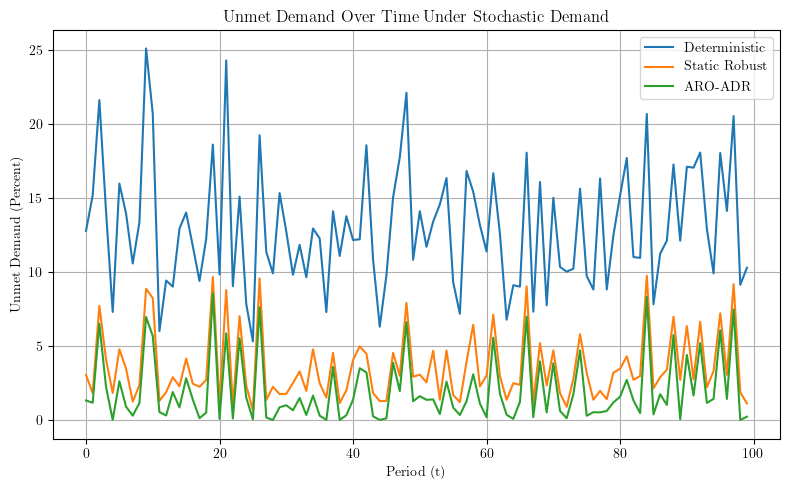
\includegraphics[width=\linewidth]{unmetdemandgabs.png}
        \caption{Unmet antimicrobial demand percentages in Gaborone over 100 
        decision epochs under stochastic demand generated from the Medical 
        Demand Estimator (MDE).}
        \label{fig:unmetdemandgabs}
    \end{minipage}
    \hfill
    \begin{minipage}[b]{0.48\linewidth}
        \centering
        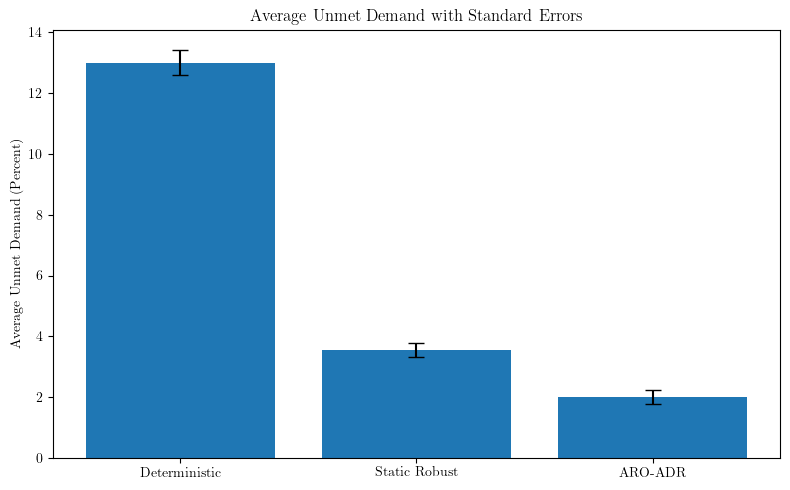
\includegraphics[width=\linewidth]{unmetdemandaverage100gabs.png}
        \caption{Average unmet demand percentage over 100 epochs and multiple 
        stochastic demand realizations (mean $\pm$ standard error).}
        \label{fig:averagesgabs}
    \end{minipage}
\end{figure}

As shown in Figures~\ref{fig:unmetdemandgabs} and \ref{fig:averagesgabs}, the three policies produce markedly different service outcomes. The deterministic policy exhibits substantial period-to-period volatility, with unmet demand frequently exceeding 20\% and averaging approximately 
13\% across the simulation horizon. This reflects the fundamental vulnerability of nominal planning to demand shocks: without any hedging mechanism, shortages arise whenever realized demand exceeds the planned allocation.

The static robust policy substantially dampens these shortfalls, reducing average unmet demand to approximately 3.6\% by conservatively pre-positioning stock against worst-case demand deviations. This comes at the cost of higher procurement spend, as the policy must buffer against uncertainty without the ability to adapt once shipments are fixed.

The ARO--ADR policy achieves the best service performance, reducing average unmet demand further to approximately 2.0\%. Critically, this improvement is achieved with only a marginal increase in procurement cost relative to the static robust policy, as a 1.5\% increase in procurement spend yields a 42\% reduction in unmet demand units. This asymmetry highlights the core value of adjustable robustness: by allowing shipments to respond to realized demand deviations, the policy extracts substantially greater service reliability from a marginally higher procurement budget.

\begin{figure}
    \centering
    \begin{minipage}[b]{0.48\linewidth}
        \centering
        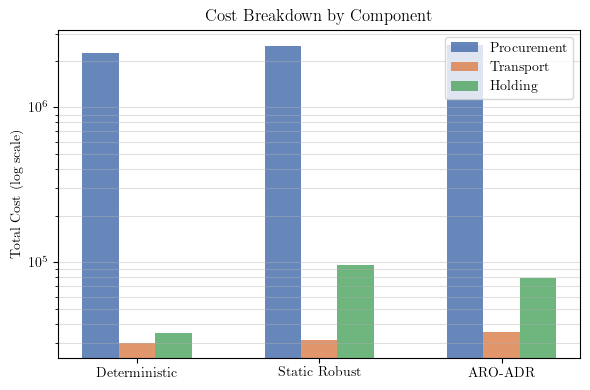
\includegraphics[width=\linewidth]{costbreakdown.png}
        \caption{Cost breakdown by component (procurement, transport, 
        holding) across policies.}
        \label{fig:costbreakdown}
    \end{minipage}
    \hfill
    \begin{minipage}[b]{0.48\linewidth}
        \centering
        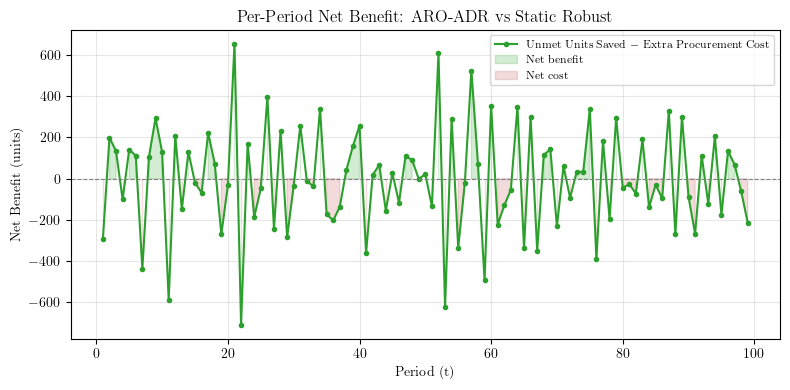
\includegraphics[width=\linewidth]{costbenefit.png}
        \caption{Cost-benefit gap between static robust and ARO--ADR: 
        additional procurement spend versus unmet demand eliminated.}
        \label{fig:costbenefit}
    \end{minipage}
    \vspace{1em}
    \begin{minipage}[b]{0.6\linewidth}
        \centering
        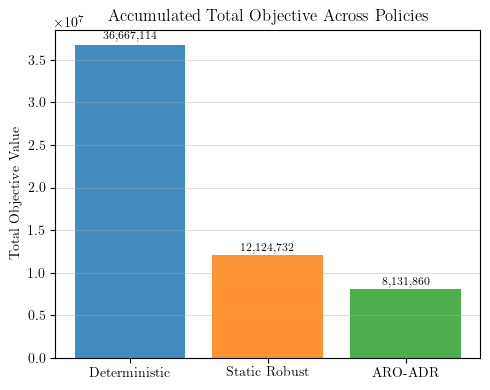
\includegraphics[width=\linewidth]{objectivecomparison.png}
        \caption{Average total objective value across policies.}
        \label{fig:objectivecomparison}
    \end{minipage}
\end{figure}

Figure~\ref{fig:objectivecomparison} confirms that ARO--ADR achieves the lowest total objective value, reducing it by approximately 33\% relative to static robust and by over 75\% relative to the deterministic policy. This reduction is driven primarily by the sharp drop in unmet demand penalties, which dominate the objective given the shortage penalty of 100 per unit. Figure~\ref{fig:costbreakdown} contextualizes this: while robust policies incur higher procurement and holding costs than the deterministic baseline, these are modest relative to the shortage costs they avoid. The log scale reveals that transport costs are broadly similar across all three policies, suggesting that the performance gap is almost entirely attributable to inventory and allocation decisions rather than routing. Figure~\ref{fig:costbenefit} shows the per-period net benefit of ARO--ADR over static robust, defined as unmet demand units saved minus additional procurement cost (which is normalized at 1.0 per drug in our simulation runs). The net benefit is positive in the majority of periods, with the negative periods reflecting isolated episodes where ARO--ADR procures more than it immediately recovers in service improvement. The cumulative picture is strongly positive, reinforcing that adaptive recourse extracts substantial service gains at modest incremental cost.

\begin{figure}
    \centering
    \begin{minipage}[b]{0.48\linewidth}
        \centering
        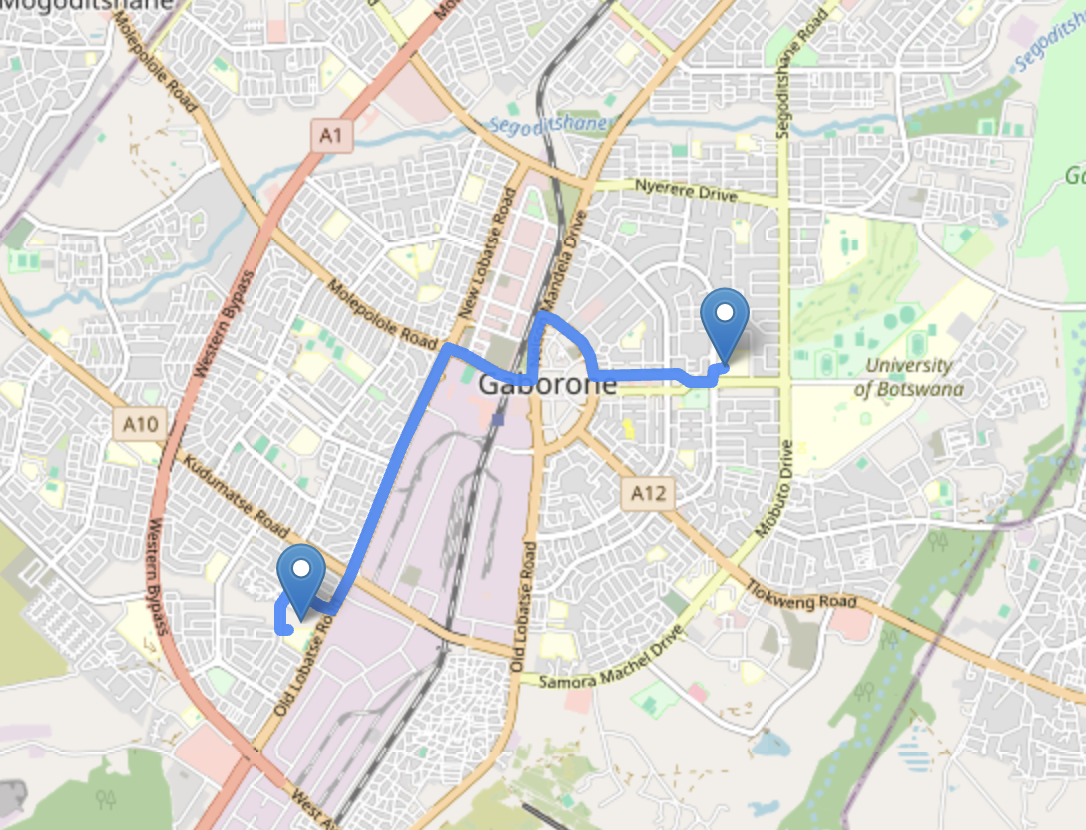
\includegraphics[width=\linewidth]{cmstopmh.png}
        \caption{Optimal route from Central Medical Stores (CMS) to 
        Princess Marina Hospital.}
        \label{fig:cmspmh}
    \end{minipage}
    \hfill
    \begin{minipage}[b]{0.48\linewidth}
        \centering
        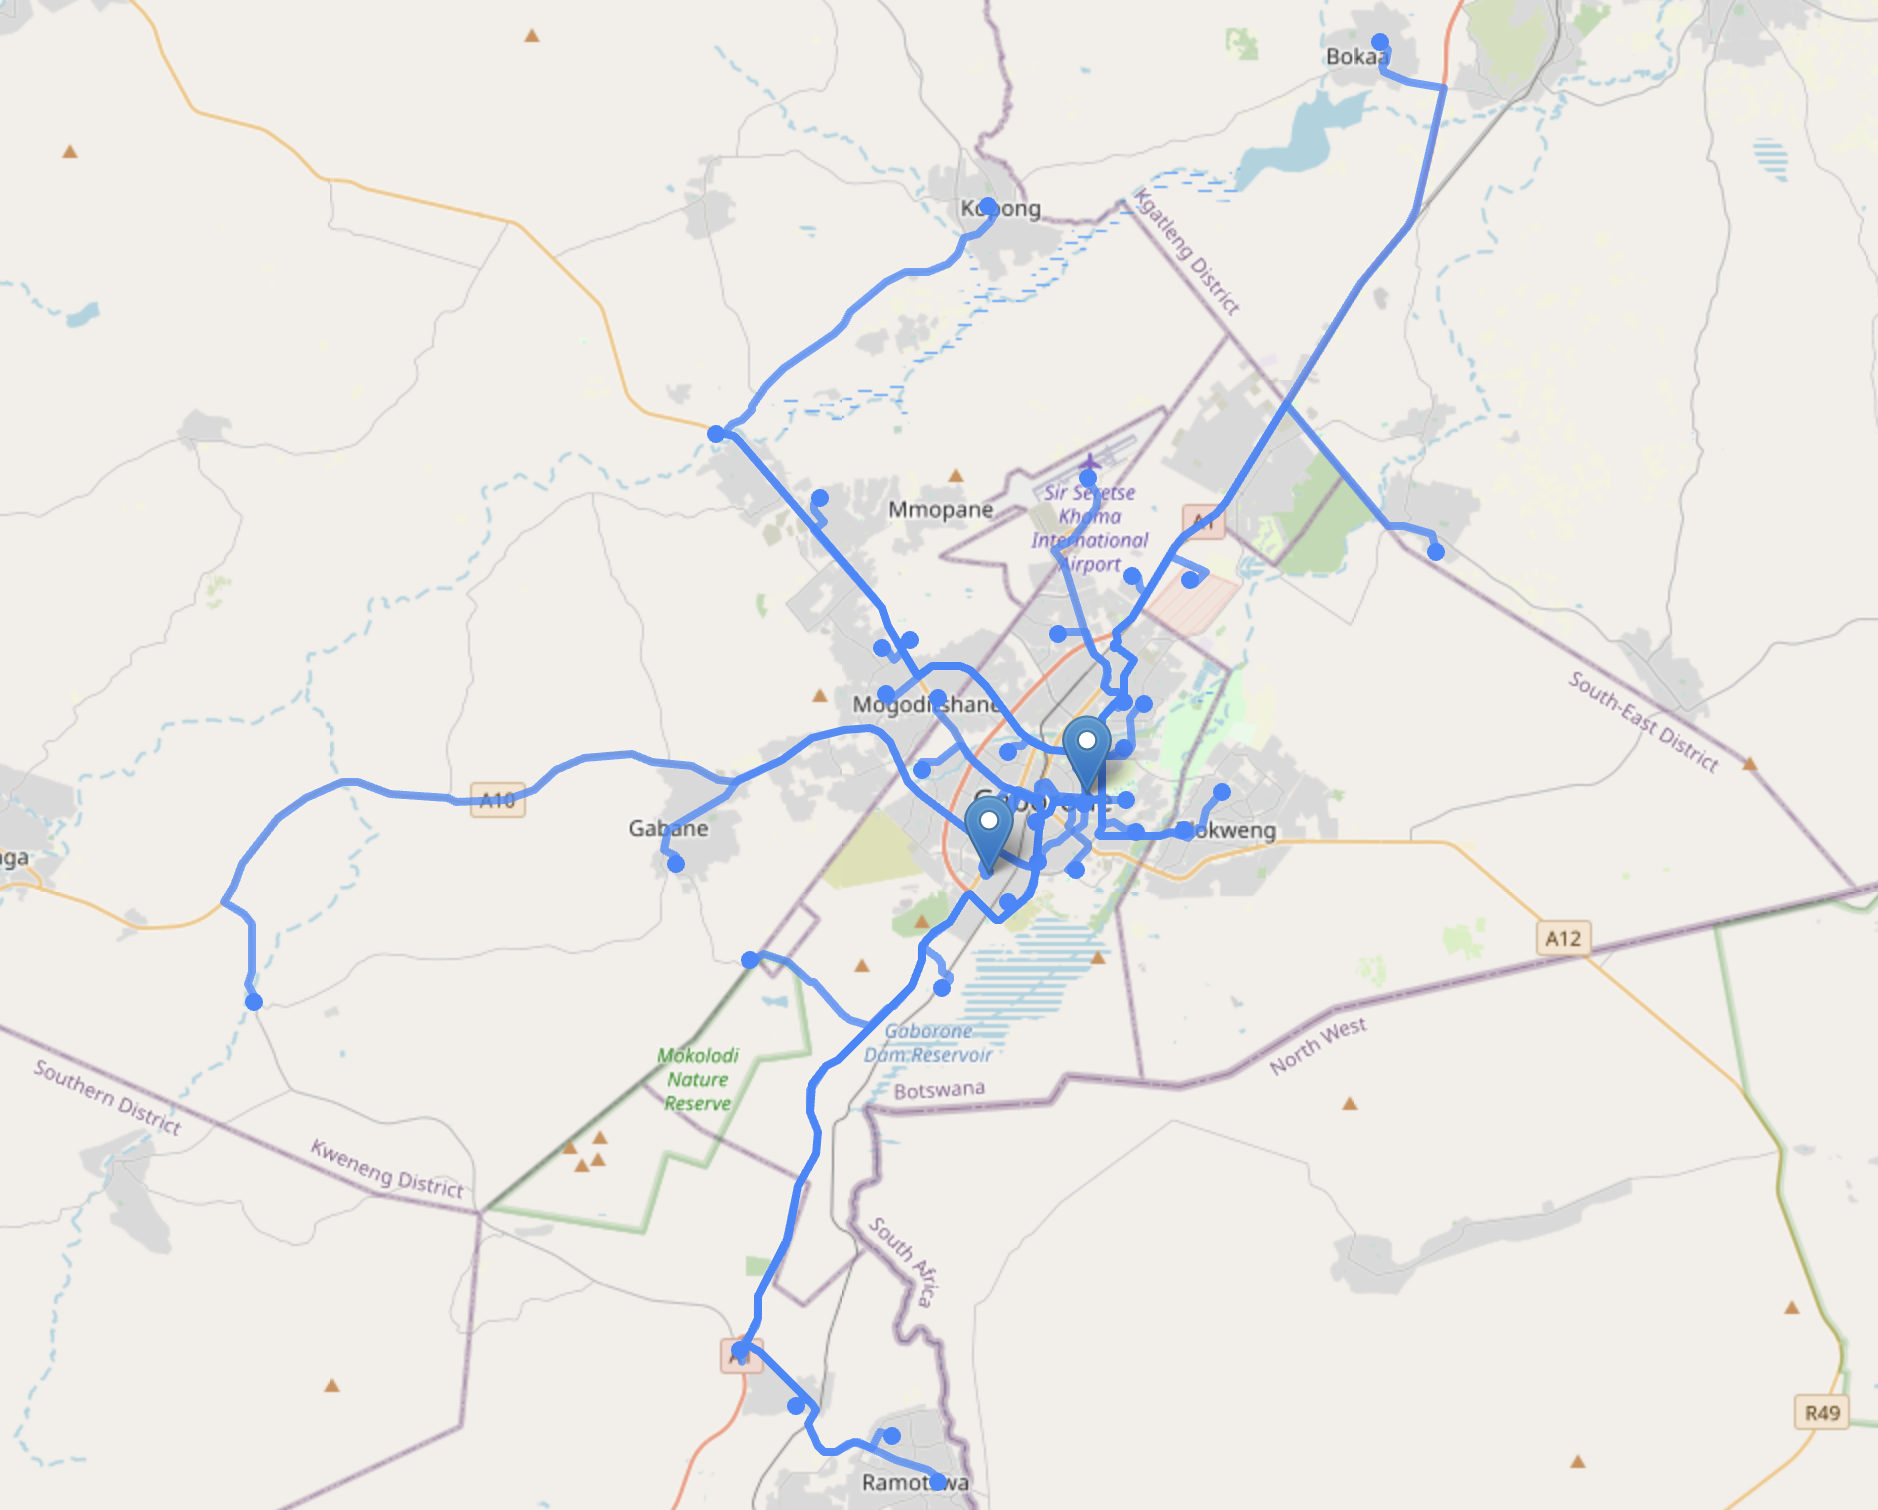
\includegraphics[width=\linewidth]{gabsmultiechelon.png}
        \caption{Optimal multiechelon network from CMS to Princess Marina 
        Hospital and downstream clinics and health posts.}
        \label{fig:cmspmhdownstream}
    \end{minipage}
\end{figure}

The optimal routing structure is illustrated in 
Figures~\ref{fig:cmspmh} and \ref{fig:cmspmhdownstream}. The direct CMS--PMH route serves as the primary supply artery, while the broader multiechelon network distributes stock onward to downstream clinics and health posts. The bidirectional flow structure allows excess inventory at lower-tier facilities to be returned upstream, reducing waste and improving system-wide allocation efficiency.

\subsubsection{Sensitivity Analysis}
\label{sens}

\begin{figure}
    \centering
    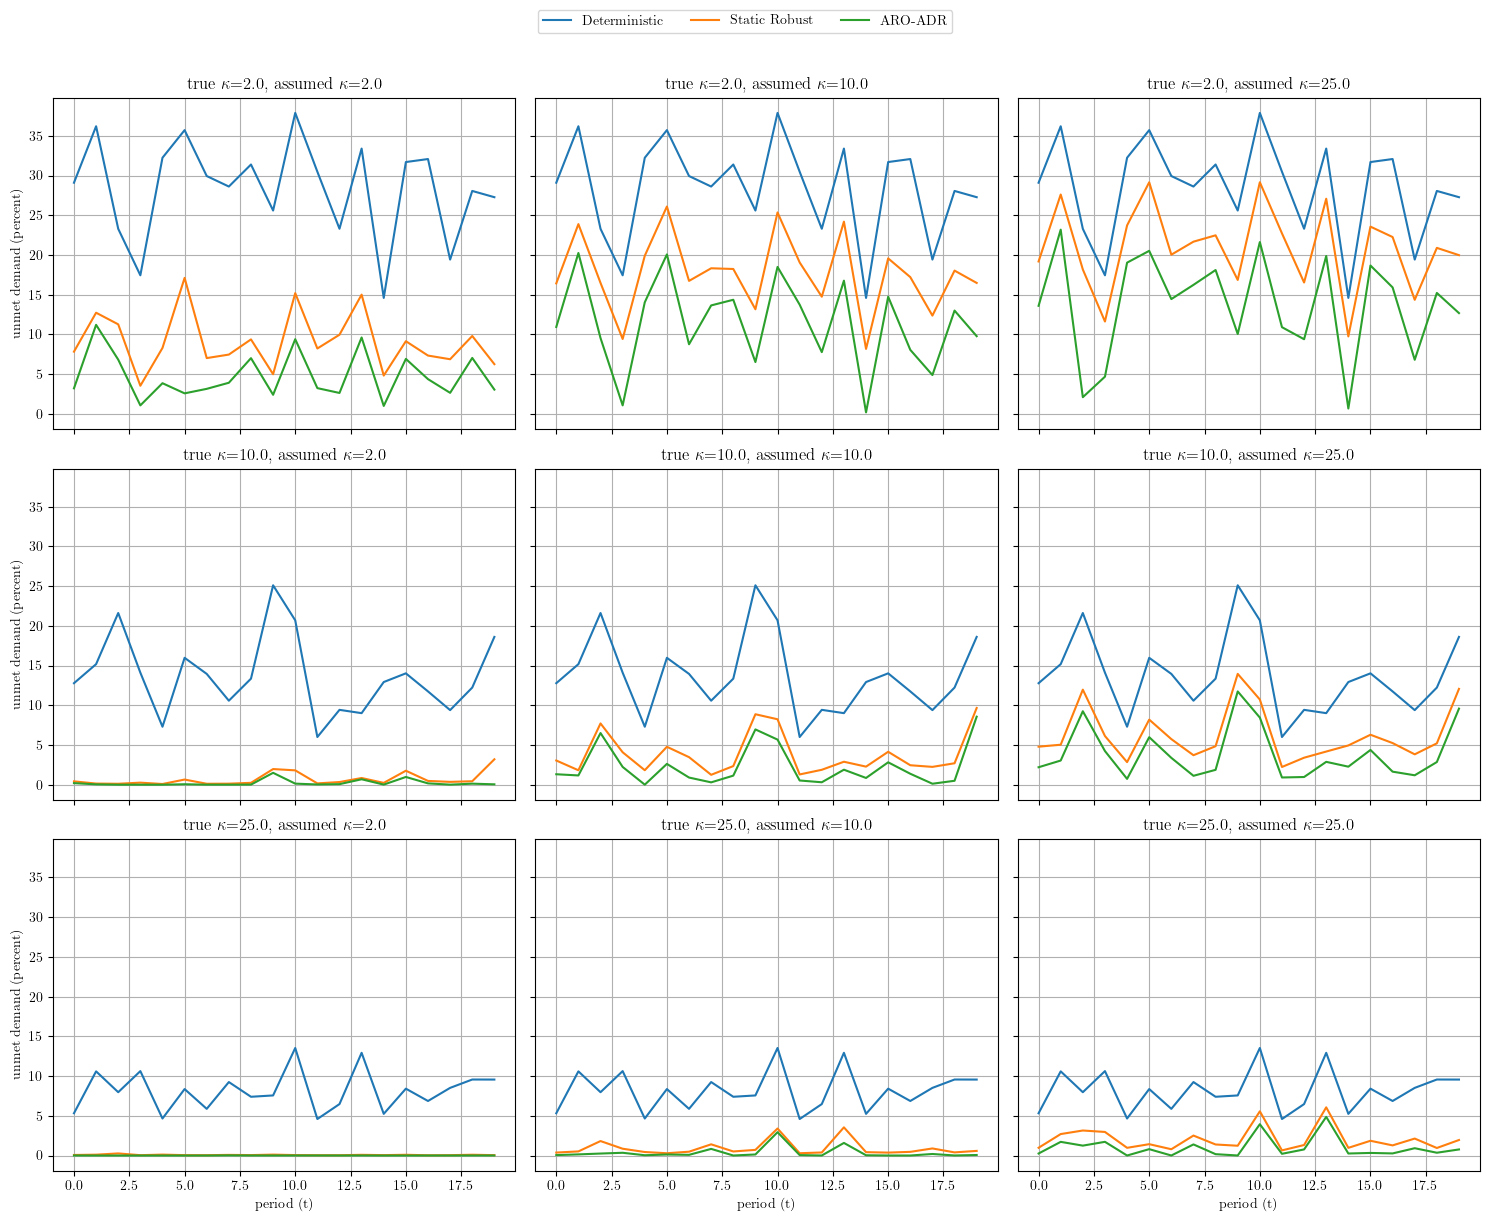
\includegraphics[width=0.9\linewidth]{kappa.png}
    \caption{Unmet demand trajectories under true and assumed values of 
    the dispersion parameter $\kappa$. Rows correspond to the true 
    $\kappa$ governing demand generation; columns correspond to the 
    assumed $\kappa$ used to calibrate $\sigma_{n,k}^{(t)}$ and the 
    uncertainty set.}
    \label{fig:kappa}
\end{figure}

A key practical concern is that the dispersion parameter $\kappa$ governing the Negative Binomial demand model must be estimated from data and may be incorrectly specified. Since $\sigma_{n,k}^{(t)}$ and therefore the uncertainty set $\mathcal{U}_D$ are calibrated from $\kappa$, misspecification directly affects the hedging behavior of both robust policies. Figure~\ref{fig:kappa} reports unmet demand trajectories across a $3 \times 3$ grid of true and assumed $\kappa$ values, isolating the effect of this misspecification.

The diagonal panels (true $\kappa$ = assumed $\kappa$) represent the correctly specified case and confirm the baseline ordering: ARO--ADR dominates static robust, which dominates the deterministic policy across all volatility levels. As true $\kappa$ increases toward the Poisson limit, demand variability falls and all policies improve, consistent with the theoretical expectation that robust methods are most valuable under high uncertainty.

The off-diagonal panels reveal an asymmetric misspecification story. When $\kappa$ is over-assumed relative to the truth (lower-left panels), the uncertainty set is too small and both robust policies under-hedge. Static robust deteriorates substantially in this regime. For instance, under true $\kappa = 2.0$ with assumed $\kappa = 10.0$, static robust unmet demand spikes to levels approaching the deterministic policy. ARO--ADR, by contrast, partially compensates through its adaptive recourse mechanism: even when the nominal uncertainty set is under-calibrated, the affine adjustment responds to realized deviations and recovers a portion of the lost service reliability.

When $\kappa$ is under-assumed (upper-right panels), both robust policies over-hedge, inflating procurement and holding costs unnecessarily. Here ARO--ADR again degrades more gracefully, as its adaptive structure naturally avoids the most conservative allocations when realized demand is less volatile than anticipated.

Taken together, these results suggest that ARO--ADR is robust not only to demand uncertainty but also to misspecification of the uncertainty set itself. This is a practically important property: since $\kappa$ must be estimated from limited data, in this case a single point prevalence survey, a policy that performs well across a range of assumed $\kappa$ values provides stronger operational guarantees than one requiring precise calibration.

To complement the distributional misspecification analysis, we examine how the uncertainty budget $\Gamma$ affects realized policy performance. Fixing the true demand distribution and varying $\Gamma \in \{1, 5, 10, 20, 50\}$ across dispersion levels $\kappa \in \{2, 10, 25\}$, Appendix Figure~\ref{fig:gamma_sensitivity} reports realized unmet demand (\%) for the Deterministic, Static Robust, and ARO-ADR policies across all $3 \times 5 = 15$ configurations.

Two patterns emerge. First, as $\kappa$ increases, reflecting more concentrated and less overdispersed demand, all three policies converge in performance. This is because  demand realizations cluster tightly around the mean and leave little room for distributional hedging to add value. Second, the gap between ARO-ADR and Static Robust narrows monotonically as $\Gamma$ grows. At $\Gamma = 1$, ARO-ADR substantially outperforms Static Robust, particularly under high demand uncertainty (low $\kappa$). At $\Gamma = 50$, the two policies are nearly indistinguishable.

This convergence is theoretically sound. The ADR allows recourse decisions to adapt to observed demand realizations, but as $\Gamma$ grows, the robust optimization worst-cases over an increasingly large uncertainty set. The optimizer therefore suppresses the adaptive component of the policy as any adaptation can be exploited by a sufficiently adversarial scenario, and in the limit the ADR collapses to a static decision rule, recovering the Static Robust solution. The empirical convergence in Figure~\ref{fig:gamma_sensitivity} thus serves as a consistency check on the implementation, and further investigation could potentially derive theoretical results for this convergence.

Taken together, these results suggest that the value of adaptivity is highest in a specific regime: low $\kappa$ (high demand variability) and moderate $\Gamma$ (sufficient but not excessive conservatism). This interaction between distributional uncertainty and the uncertainty budget constitutes a practical guideline for calibrating robust policies in pharmaceutical supply chains.

\subsubsection{Seasonality}

Seasonal variation in disease burden is a challenge for health supply chains, particularly in settings where demand for treatments fluctuates predictably throughout the year. For tuberculosis in Southern Africa, \cite{ballif2018} documented recurring monthly fluctuations in PTB diagnoses at ART programmes across South Africa and Zimbabwe, driven primarily by seasonal changes in clinical activity and health-seeking behaviour rather than climatic factors. Peaks in diagnoses occur in January--February following the December holiday period, with a secondary trough in April--May corresponding to Easter. Failure to account for such patterns in supply planning can lead to systematic stockouts during high-demand periods and wasteful overstocking during low-demand periods, both of which carry significant costs in resource-constrained settings. Robust optimization-based models are particularly well-suited to capturing this structure, as the uncertainty set can be constructed around a time-varying mean rather than a stationary one.

To stress-test the proposed supply chain model under non-stationary demand, we restrict attention to the three antibiotic classes most directly associated with drug-resistant tuberculosis treatment: aminoglycosides, quinolones, and lincosamides. These classes correspond to second-line agents used in MDR-TB and XDR-TB regimens, for which the seasonal demand pattern documented by \cite{ballif2018} is most clinically consequential. We assume that drug dispensing demand for these classes follows the same seasonal pattern as TB diagnosis counts and model demand at each facility as a seasonally-adjusted negative binomial process. Specifically, the mean demand at node $n$ for drug class $k$ in period $t$ is given by

\begin{equation}
    \tilde{\mu}_{n,k}^{(t)} = s(t) \cdot \mu_{n,k}
\end{equation}

where $\mu_{n,k}$ is the baseline mean demand and $s(t)$ is a seasonal multiplier defined by a two-harmonic Fourier approximation:

\begin{equation}
    s(t) = 1 + A_1 \sin\!\left(\frac{2\pi t}{P} + \frac{\pi}{2}\right) 
             + A_2 \sin\!\left(\frac{4\pi t}{P} - \frac{\pi}{4}\right)
\end{equation}

where $P = 26$ is the length of the seasonal cycle in fortnightly periods. The amplitudes $A_1 = 0.7249$ and $A_2 = -0.5585$ are calibrated by solving 
the system of equations $s(1) = 1.87$ and $s(13) = 0.67$, reproducing the $+87\%$ January peak and $-33\%$ December trough reported for the Zimbabwe (Newlands) site in \cite{ballif2018}. The resulting multiplier pattern is shown in Figure~\ref{fig:seasonal_analysis}(c). The multiplier satisfies $s(t) > 0$ for all $t \in \{0, \ldots, 25\}$ and has mean approximately equal to unity over a full cycle, preserving the baseline annual demand. We note that the April--May secondary trough emerges as an artefact of the functional form rather than a separately calibrated target, and is deeper than the December trough; this is a known limitation of the two-harmonic approximation.

Demand realisations $d_{n,k}^{(t)}$ are drawn independently each period from a negative binomial distribution:

\begin{equation}
    d_{n,k}^{(t)} \sim \text{NegBin}\!\left(\tilde{\mu}_{n,k}^{(t)},\, \kappa\right)
\end{equation}

where $\kappa > 0$ is the dispersion parameter. We set $\kappa = 50$, corresponding to low overdispersion, in order to isolate the effect of the seasonal signal without allowing stochastic noise to obscure the comparative performance of the three policies. The variance of $d_{n,k}^{(t)}$ is $\tilde{\mu}_{n,k}^{(t)} + \left(\tilde{\mu}_{n,k}^{(t)}\right)^2 / \kappa$, so that smaller values of $\kappa$ correspond to greater overdispersion relative to a Poisson process. The standard deviation used in the robust uncertainty set is therefore

\begin{equation}
    \sigma_{n,k}^{(t)} = \sqrt{\tilde{\mu}_{n,k}^{(t)} + \frac{\left(\tilde{\mu}_{n,k}^{(t)}\right)^2}{\kappa}}
    \label{eq:sigma}
\end{equation}

Figure~\ref{fig:seasonal_analysis} summarizes the seasonal stress-test. Panels~(a) and~(b) both show unmet demand over two full cycles ($T = 52$) under the same seasonally-varying demand realisations, but differ in what information is supplied to the optimizer. In panel~(a), the optimizer is given only stationary demand estimates, with no knowledge of the seasonal pattern; all three policies are consequently caught off-guard at each peak, producing unmet demand spikes exceeding 50\% at $t \approx 25$ and $t \approx 50$. In panel~(b), the optimizer is supplied with the seasonally-adjusted means $\tilde{\mu}_{n,k}^{(t)}$, allowing it to pre-position inventory ahead of anticipated surges. This reduces peak unmet demand substantially across all policies, with ARO-ADR achieving a mean unmet rate of $0.72\%$ over the full horizon, compared to $2.21\%$ for static robust and $8.39\%$ for the deterministic policy. Panel~(c) shows the calibrated multiplier $s(t)$, which rises sharply to a peak of $2.12$ in the first period of each cycle before falling to a trough near zero around $t = 18$, reflecting the January surge and mid-year lull documented by \cite{ballif2018}.

\begin{figure}[t]
    \centering
    \begin{subfigure}[b]{0.48\textwidth}
        \centering
        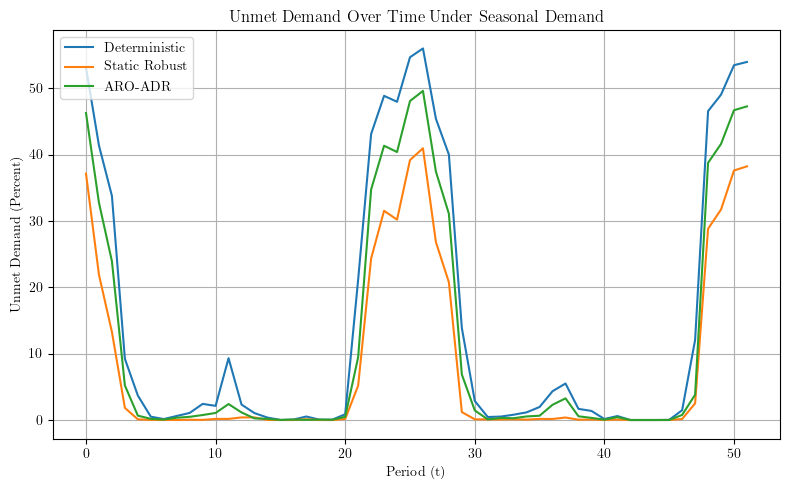
\includegraphics[width=\textwidth]{seasonal_unmet_no_multiplier.png}
        \caption{}
        \label{fig:seasonal_unmet_flat}
    \end{subfigure}
    \hfill
    \begin{subfigure}[b]{0.48\textwidth}
        \centering
        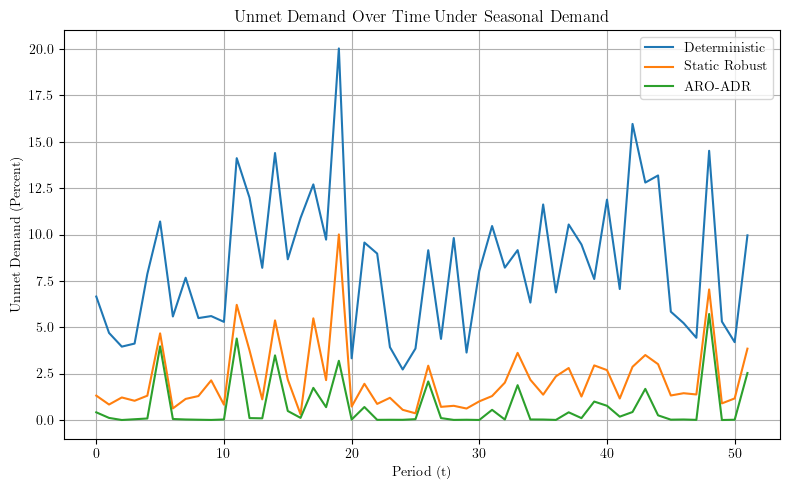
\includegraphics[width=\textwidth]{seasonal_unmet_with_multiplier.png}
        \caption{}
        \label{fig:seasonal_unmet_seasonal}
    \end{subfigure}
    
    \vspace{0.5em}
    
    \begin{subfigure}[b]{0.48\textwidth}
        \centering
        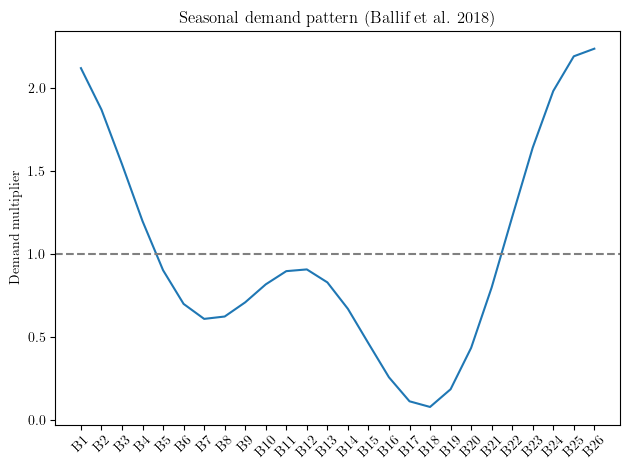
\includegraphics[width=\textwidth]{seasonal_multiplier.png}
        \caption{}
        \label{fig:seasonal_multiplier}
    \end{subfigure}
    \caption{Seasonal demand analysis over two cycles ($T = 52$ fortnightly periods). Panels~(a) and~(b) show realized unmet demand (as a percentage of total demand) across the deterministic, static robust, and ARO-ADR policies, under flat and seasonally-adjusted demand estimates respectively. When the optimizer is supplied only with stationary demand estimates, all three policies fail to anticipate seasonal peaks, producing unmet demand spikes exceeding 50\% at $t \approx 25$ and $t \approx 50$. Incorporating the seasonal multiplier into the uncertainty set dramatically reduces these spikes, with ARO-ADR achieving a mean unmet rate of $0.72\%$ compared to $2.21\%$ for static robust and $8.39\%$ for the deterministic policy. Panel~(c) shows the two-harmonic Fourier multiplier $s(t)$ calibrated to the Zimbabwe (Newlands) site in \cite{ballif2018}.}
    \label{fig:seasonal_analysis}
\end{figure}

It should be noted that this seasonal specification is not intended as a precise empirical model of Botswana's antimicrobial demand. Botswana's clinical context, health-seeking behavior, and holiday calendar differ from the Zimbabwean site in \cite{ballif2018}, and a sinusoidal functional form is an obvious simplification of any real seasonal pattern. Rather, the purpose of this experiment is to stress-test the robust optimization framework under a plausible and structured form of non-stationarity. The key question is not whether the seasonal pattern is precisely correct, but whether the ARO-ADR policy remains robust to demand that varies systematically over time, a property that a stationary uncertainty set does not guarantee. The Zimbabwe figures serve only to ground the amplitude of the seasonal variation in an empirically observed order of magnitude.

A practical consideration for implementation is that the robust uncertainty set requires estimates of $\sigma_{n,k}^{(t)}$ at each node, drug class, and period. In our formulation, these are derived analytically from the seasonally-adjusted mean $\tilde{\mu}_{n,k}^{(t)}$ and the dispersion parameter $\kappa$ via equation~\eqref{eq:sigma}. In practice, the Central Medical Stores would not have access to these parameters directly. However, both $\mu_{n,k}$ and $\kappa$ can be estimated from historical dispensing records using standard negative binomial regression, and the seasonal multiplier $s(t)$ can be fitted from longitudinal consumption data. Once estimated, these parameters can be stored and updated periodically, requiring no real-time data collection beyond what is already captured in routine stock management systems. Additionally, an alternative way to account for this may be to err on the side of conservatism in ensuring drug demand quotas are fulfilled, as found in our sensitivity analyses of $\kappa$.

\subsection{Botswana Trial}
\subsubsection{National Adaptation}
\label{botswananatadap}

The national trial extends the Gaborone proof-of-concept to all health districts in Botswana, solving a separate multiechelon optimization problem for each district. This district-level decomposition is motivated by both computational and equity considerations. A single national MIP would be computationally difficult at the scale of 631 facilities across multiple drug classes. More importantly, a fully centralized formulation would allow the optimizer to concentrate allocations toward high-demand urban facilities at the expense of rural health posts: when distances are long and population centers are unequally distributed, a cost-minimizing solver will naturally favor routes serving large nearby populations over those serving sparse remote ones. Solving districts independently ensures that each district receives dedicated optimization attention, preserving geographic equity across Botswana's highly heterogeneous facility landscape. In addition to the district-level decomposition, the integrality constraints on the vehicle dispatch variables are relaxed to their linear programming counterparts at national scale, replacing the binary and integer variables with continuous ones. This relaxation is necessary to keep individual district subproblems tractable given the larger node and arc counts encountered outside Gaborone.

At national scale, inter-facility distances are substantially longer than in the Gaborone trial, increasing transport costs and raising the stakes of misallocation. This makes adaptive recourse more valuable, since correcting a poor initial shipment decision is costlier when facilities are further apart.

A further distinction from the Gaborone trial concerns the treatment of rural census districts that could not be directly geocoded. As described in Section~\ref{popfacgeocoding}, these districts were assigned approximate locations by drawing uniformly over rectangular regions covering their approximate boundaries, and then matched to their nearest health facility. In the Gaborone trial this was largely inconsequential, as the district is predominantly urban and few facilities lacked coordinates. At national scale, however, ungeocoded districts are disproportionately rural and sparse, and their demand contribution becomes materially relevant to the allocation problem.

\subsubsection{National Results on Simulation Runs}

\begin{figure}
    \centering
    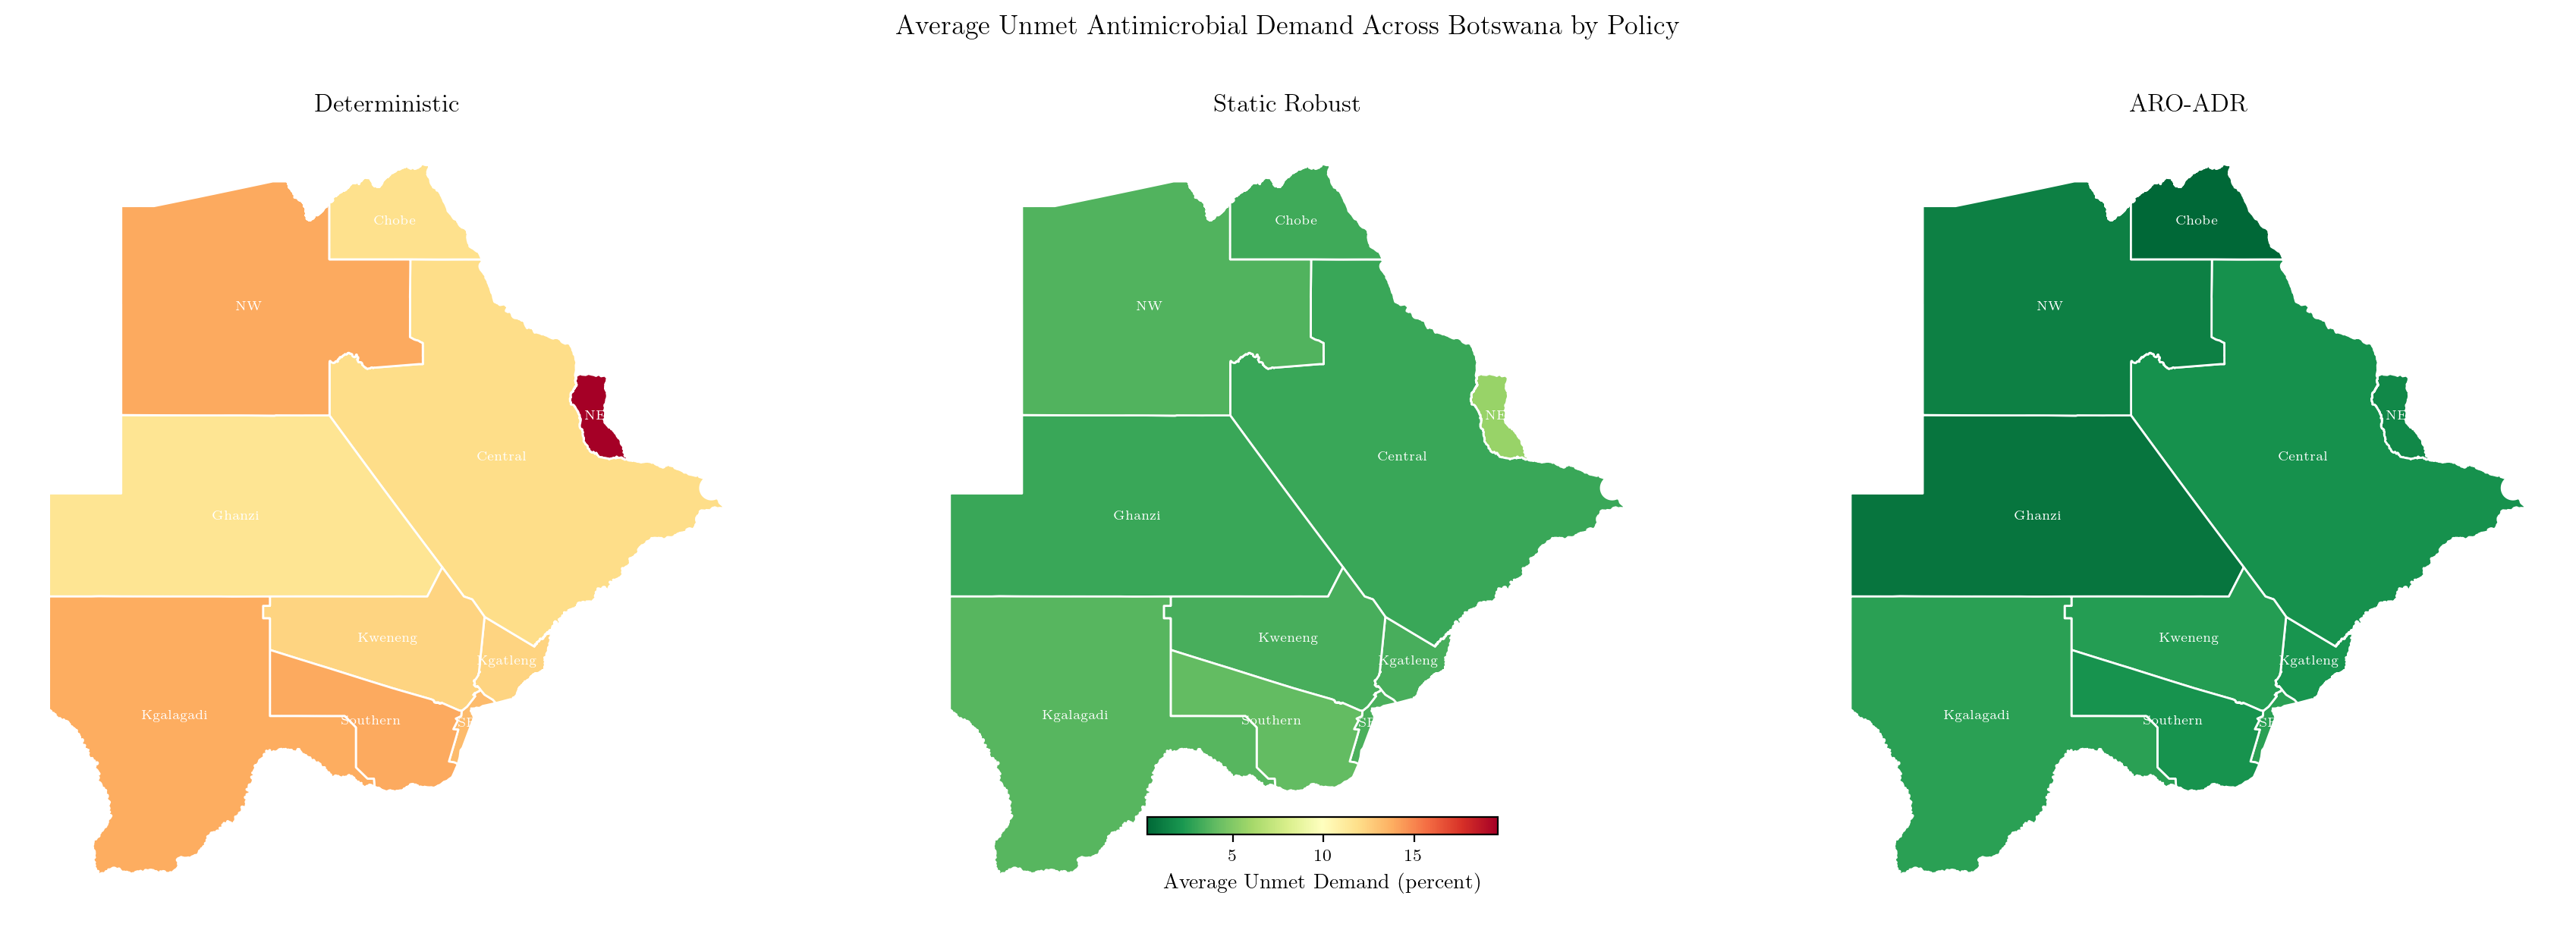
\includegraphics[width=1\linewidth]{botswana_heatmap.png}
    \caption{Average unmet demand across Botswana districts under all three policies (T=20)}
    \label{fig:botswana_heatmap}
\end{figure}

Table~\ref{tab:national_results} summarizes average per-period performance across all 18 districts under the three policies. The national results closely mirror the Gaborone proof-of-concept, providing out-of-sample validation that the policy ordering is robust to geographic scale and network heterogeneity.

\begin{table}[h]
\centering
\begin{tabular}{lccc}
\hline
Policy & Avg.\ Unmet Demand (\%) & Avg.\ Procurement Cost & Avg.\ Objective \\
\hline
Deterministic  & 13.48 & 21{,}266 & 318{,}473 \\
Static Robust  & 3.61  & 23{,}744 & 101{,}689 \\
ARO-ADR        & 1.88  & 23{,}967 & 75{,}072  \\
\hline
\end{tabular}
\caption{Average per-period performance across all 18 Botswana districts.}
\label{tab:national_results}
\end{table}

The deterministic policy leaves 13.5\% of demand unmet on average, consistent with its inability to hedge against realized demand shocks. Static robust reduces this to 3.6\% through conservative pre-positioning, at a modest increase in procurement cost of approximately 11.7\% relative to the deterministic baseline. ARO-ADR reduces unmet demand further to 1.9\%, achieving a 76\% reduction relative to deterministic and a 48\% reduction relative to static robust, while incurring only a 0.9\% procurement cost premium over static robust. The total objective under ARO-ADR is 26\% lower than static robust and 76\% lower than deterministic, driven primarily by avoided shortage penalties.

As shown in Figure~\ref{fig:botswana_heatmap}, the geographic distribution of unmet demand under ARO-ADR is notably uniform across districts, suggesting that adaptive recourse not only improves aggregate service levels but also reduces spatial inequality in antimicrobial access. The North-East district is a persistent outlier across all three policies, likely reflecting its small geographic footprint and concentrated demand structure, which limits the flexibility of any allocation policy.

The district-level decomposition of costs is examined in the Appendix by Figure~\ref{fig:botswana_appendix_simulation_maps}, which presents choropleth maps for all cost components across the three policies. These cost components yield some notable patterns.

Procurement costs are broadly similar across all three policies at the national level, with Kweneng consistently registering the highest procurement spend reflecting its high population density as the district surrounding Gaborone. The modest procurement premium of robust policies over the deterministic baseline is visible but geographically uniform, suggesting that the hedging cost is distributed evenly rather than concentrated in particular districts.

Transport costs reveal a more nuanced picture. Under ARO-ADR, Kweneng and Kgatleng exhibit notably higher transport costs than under static robust, reflecting the adaptive policy's potential tendency to route stock reactively in response to realized demand shocks rather than pre-positioning it statically. The trade-off of higher transport expenditure in exchange for lower shortage costs could be a direct consequence of the affine recourse mechanism.

Holding costs tell the complementary story. Static robust carries substantially more inventory than ARO-ADR, particularly in the large Central district, as it must buffer against worst-case demand without the ability to adapt. ARO-ADR reduces holding costs by redistributing stock dynamically, converting inventory slack into responsive shipments.

Finally, shortage costs confirm the aggregate results at a geographic level. The deterministic policy produces deep shortages concentrated in high-demand districts such as Kweneng, while static robust and ARO-ADR dramatically reduce shortage costs across the entire country. ARO-ADR achieves near-uniform low shortage costs nationally, reinforcing the equity finding from Figure~\ref{fig:botswana_heatmap} that adaptive recourse not only improves average performance but reduces geographic disparity in antimicrobial access, especially as unmet demand costs are tuned appropriately.

\subsubsection{National Results on CMS-Provided Data}
\label{cmsresults}

To evaluate policy performance using real procurement data, we construct facility-level demand estimates for 84 antimicrobial products using aggregate CMS dispensing records, disaggregated across facilities using catchment population proportions. Biweekly demand is derived from the average monthly consumption figures provided by CMS for the 2025--26 and 2026--27 planning horizons, with unit procurement costs drawn directly from CMS pricing records. The simulation is run independently for 11 of 18 DHMTs (District Health Management Teams) for which complete data were available, following the same district-level decomposition described in Section~\ref{botswananatadap}.

Figure~\ref{fig:cms_unmet_map} presents the average unmet antimicrobial demand across 11 of 18 DHMTs by policy and scenario across data for 84 drugs, while Figure~\ref{fig:cms_bar} summarises aggregate unmet demand with standard errors. Table~\ref{tab:cms_results} reports average unmet demand, procurement cost, and objective value by model and scenario. Full disaggregated results across all cost metrics are provided in Figures~\ref{fig:cms_full_2526} and~\ref{fig:cms_full_2627} in the Appendix.

Across both planning horizons, the ARO-ADR policy achieves the largest reductions in unmet demand, falling from 21.4\% under the deterministic policy to 3.4\% in 2025--26, and from 19.0\% to 2.7\% in 2026--27. The static robust policy offers a substantial intermediate improvement, reducing unmet demand to 7.0\% and 5.9\% respectively. These gains come at a moderate increase in procurement cost: ARO-ADR procurement costs are higher than the static robust baseline in both scenarios, reflecting the policy's willingness to pre-position stock in anticipation of demand deviations. The overall objective value is nonetheless lowest under ARO-ADR, confirming that the reduction in shortage costs more than offsets the additional procurement expenditure.

Geographically, the deterministic policy leaves Ghanzi and Kgalagadi particularly exposed, with the highest unmet demand concentrations visible in Figure~\ref{fig:cms_unmet_map}. Both the static robust and ARO-ADR policies substantially reduce shortages in these regions, with ARO-ADR achieving near-uniform low unmet demand across the country in both scenarios. The 2026--27 scenario shows a modest overall improvement relative to 2025--26 across all three policies, consistent with the lower AMC figures in the later planning horizon.

The disaggregated cost maps in Figures~\ref{fig:cms_full_2526} and~\ref{fig:cms_full_2627} reveal that the higher objective values under the deterministic policy are driven primarily by shortage costs rather than procurement or transport costs. Kweneng stands out as a high-cost outlier in transport cost across all three policies in both scenarios, likely reflecting the district's geographic size and the distances between its facilities and warehouse. Procurement costs are broadly similar across DHMTs within each policy, though Kweneng again incurs elevated procurement costs under static robust and ARO-ADR. Holding costs are generally low and uniformly distributed under the deterministic policy, but increase under static robust and ARO-ADR as these policies pre-position additional inventory to hedge against demand uncertainty. This tradeoff of higher holding costs in exchange for lower shortage costs is the central mechanism through which robust policies improve service levels, and is clearly legible across both scenarios in the Appendix figures.

\begin{table}[h]
\centering
\caption{Average unmet demand (\%), procurement cost (BWP), and objective value by model and scenario across 11 DHMTs.}
\label{tab:cms_results}
\begin{tabular}{llrrr}
\toprule
Scenario & Model & Avg.\ Unmet Demand (\%) & Avg.\ Procurement Cost & Avg.\ Objective \\
\midrule
2025--26 & Deterministic   & 21.44 & 569,334.30 & 430,194.83 \\
         & Static Robust   & 6.95  & 197,810.49 & 291,482.20 \\
         & ARO-ADR         & 3.37  & 209,776.91 & 232,998.75 \\
\midrule
2026--27 & Deterministic   & 19.00 & 228,177.22 & 564,782.55 \\
         & Static Robust   & 5.90  & 274,262.80 & 385,060.41 \\
         & ARO-ADR         & 2.74  & 290,527.21 & 317,699.75 \\
\bottomrule
\end{tabular}
\end{table}

\begin{figure}[H]
    \centering
    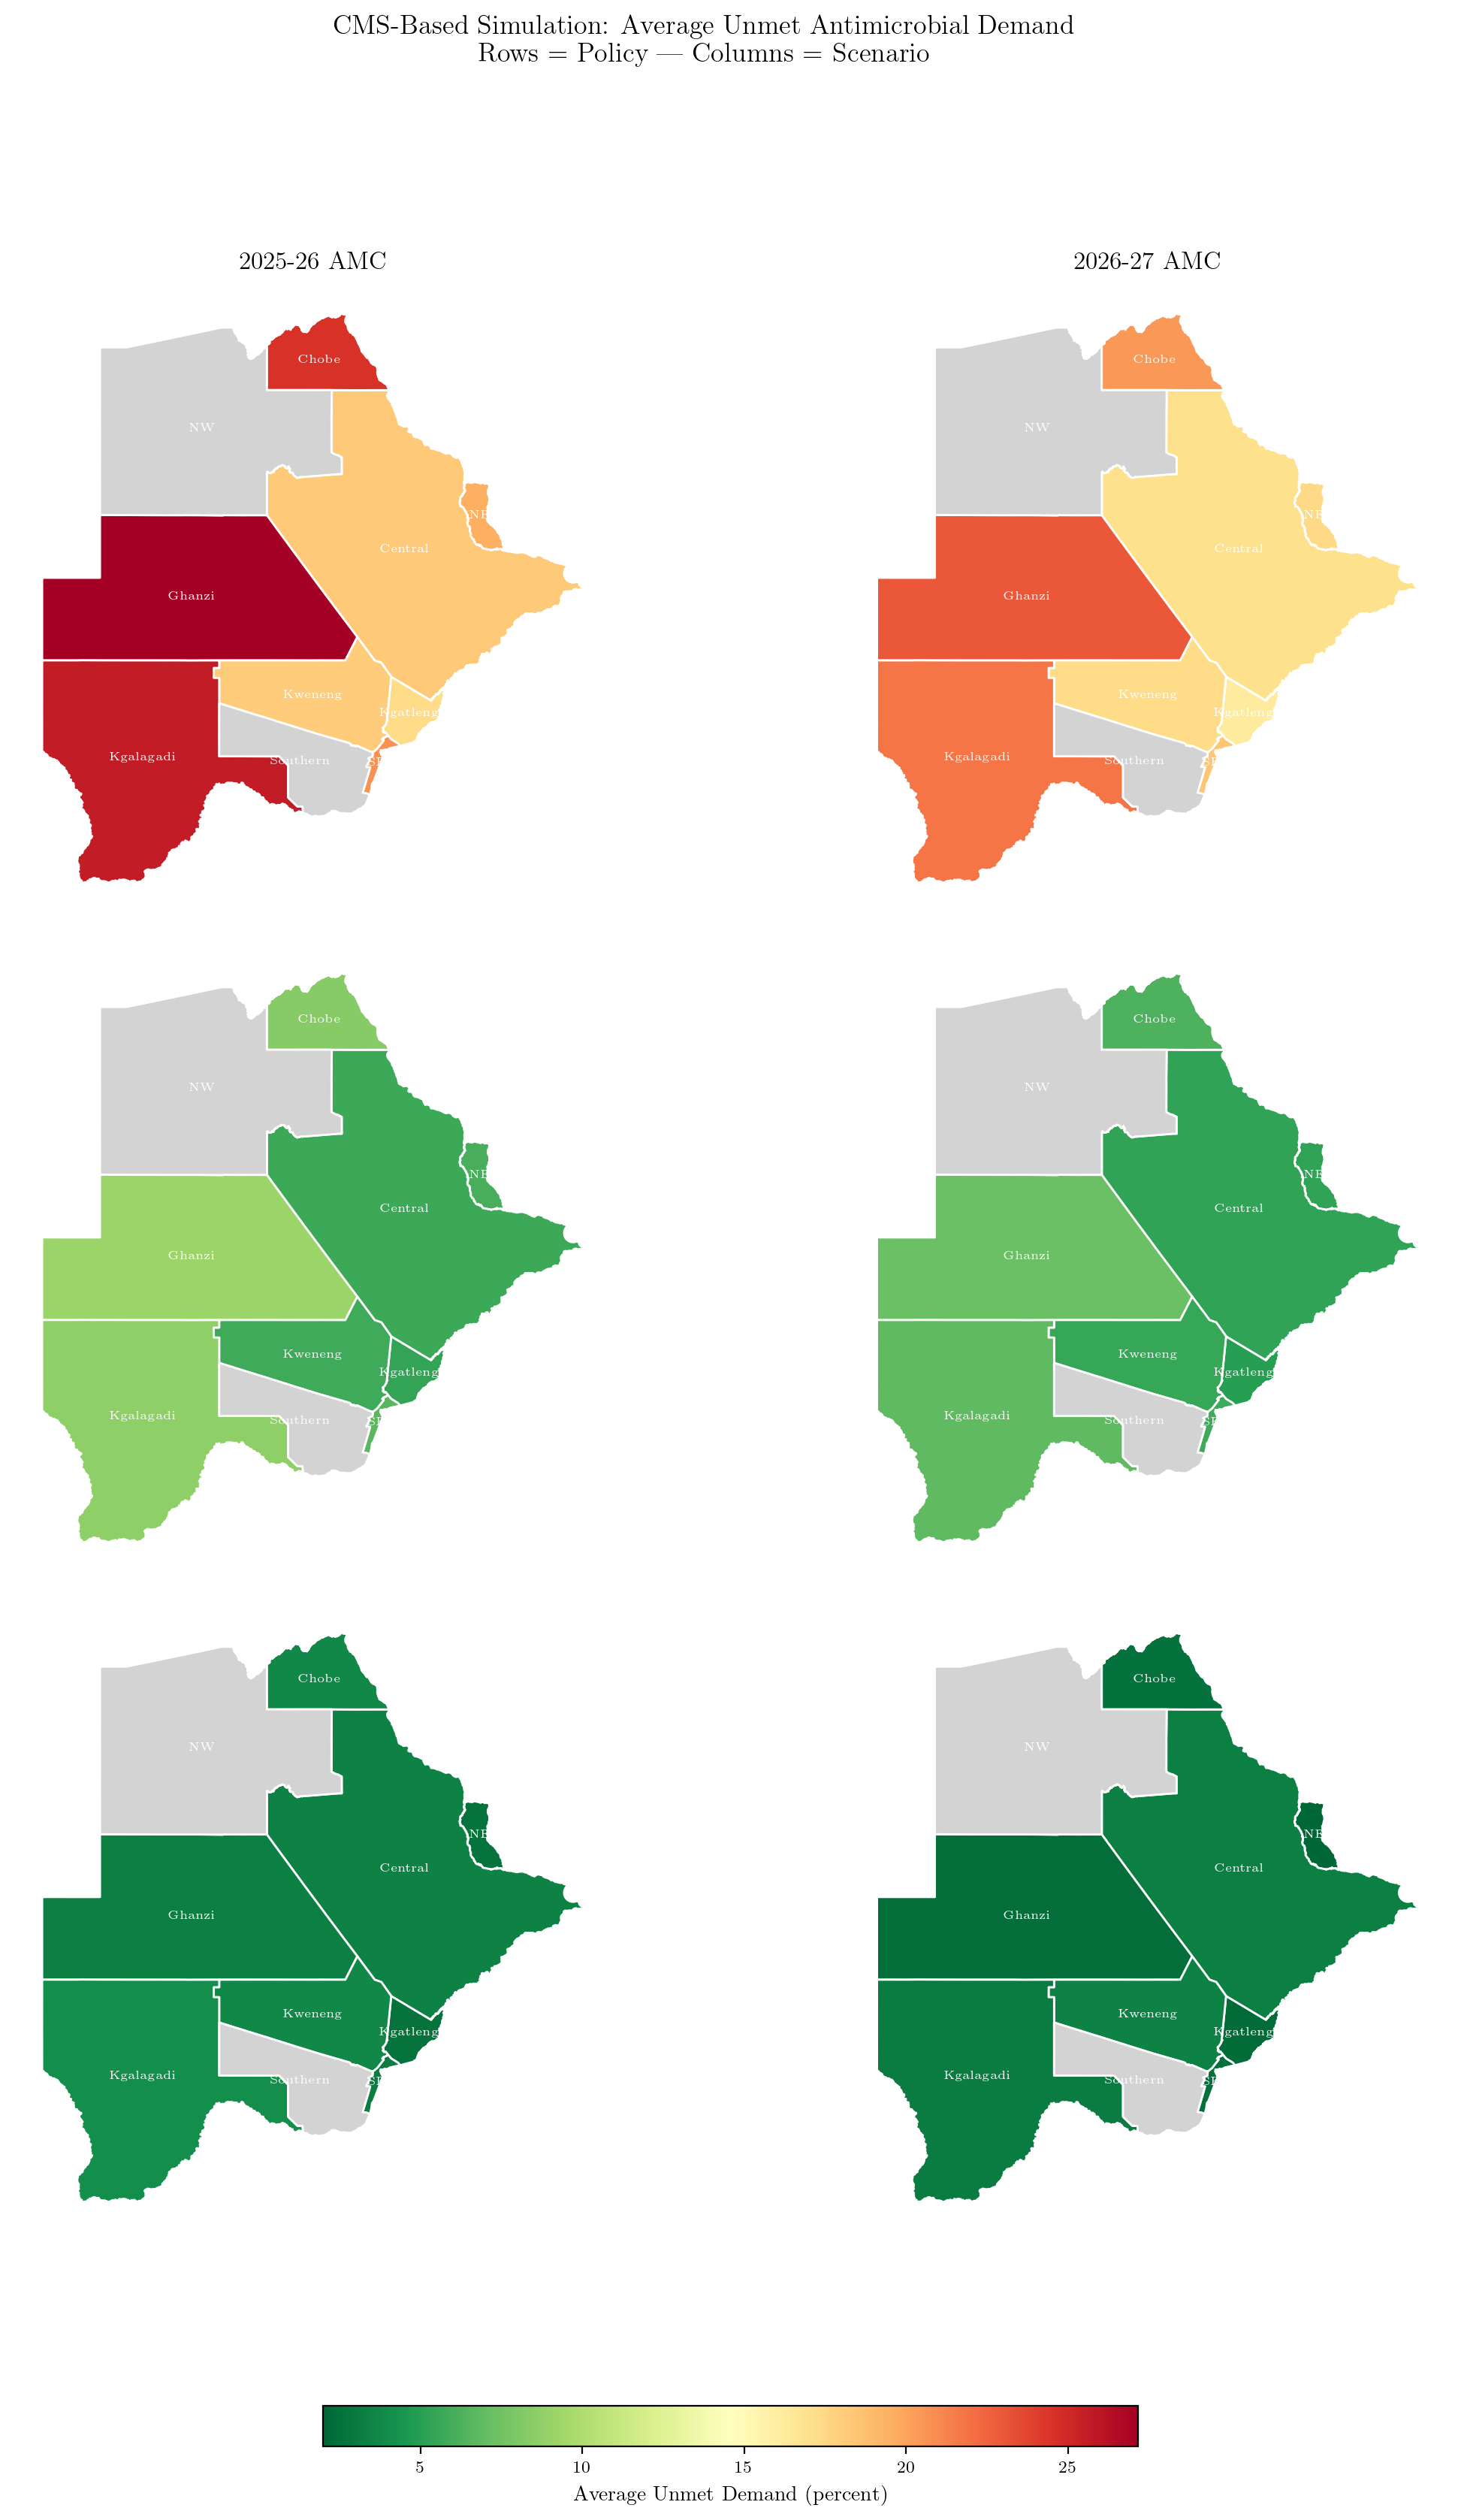
\includegraphics[width=0.6\textwidth]{cms_unmet_map.png}
    \caption{Average unmet antimicrobial demand (\%) across Botswana DHMTs by policy (rows: deterministic, static robust, ARO-ADR) and scenario (columns: 2025--26, 2026--27 AMC). Grey regions indicate DHMTs excluded due to solver and runtime constraints.}
    \label{fig:cms_unmet_map}
\end{figure}

\begin{figure}[H]
    \centering
    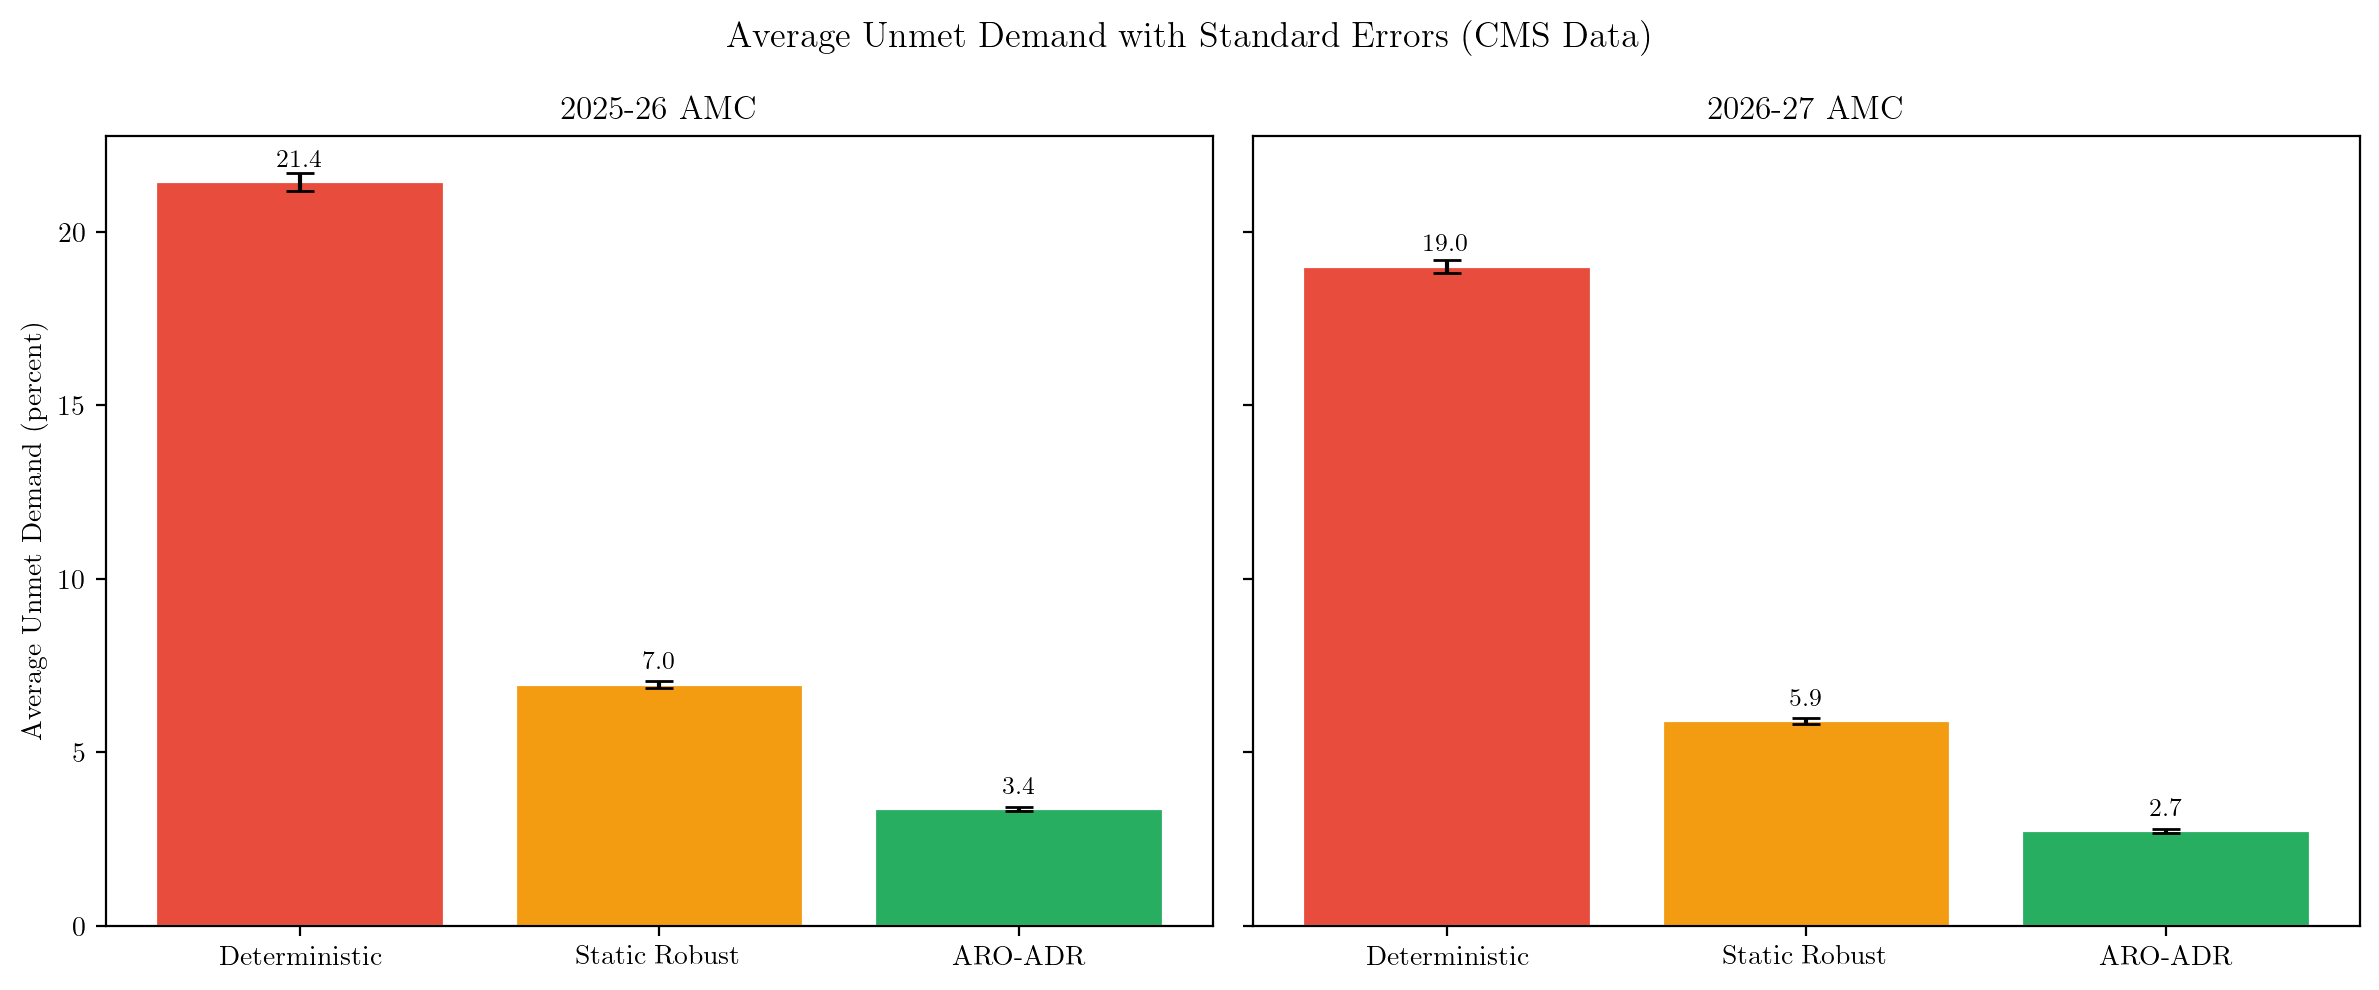
\includegraphics[width=0.6\textwidth]{cms_bar.png}
    \caption{Average unmet antimicrobial demand with standard errors under deterministic, static robust, and ARO-ADR policies for the 2025--26 and 2026--27 scenarios (CMS data, 11 DHMTs).}
    \label{fig:cms_bar}
\end{figure}

\subsection{Epidemic Demand Resilience}

\subsubsection{SEIR Framework}

To evaluate allocation policy performance under epidemic conditions, we embed a two-strain compartmental model into the simulation, calibrated to gram-negative bacterial infection dynamics at Princess Marina Hospital (PMH) in Gaborone. PMH is the primary referral hospital served by the Gaborone district network in our model and is the site of the CMS-to-facility flows examined in Section 5.2. The pathogen of focus is \textit{Klebsiella pneumoniae}, which accounts for two-thirds of bloodstream infections at PMH \cite{gezmu2020}, and which has been identified as the dominant organism in hospital-acquired extended-spectrum cephalosporin-resistant Enterobacterales (ESCrE) colonisation at the same facility \cite{ntereke2026}. The drug scope is restricted to cephalosporins as first-line therapy for the drug-susceptible (DS) strain and carbapenems as second-line therapy for the drug-resistant (DR) strain, both of which are present in the CMS dataset.

\subsubsection{State Variables}

The hospital population is partitioned into six compartments:
\[
S, \quad E_s, \quad I_s, \quad E_r, \quad I_r, \quad R
\]
representing susceptible, exposed-DS, infectious-DS, exposed-DR, infectious-DR, and 
recovered individuals respectively. Total population is 
$N = S + E_s + I_s + E_r + I_r + R$, approximated by the hospital's inpatient 
census.

\subsubsection{Transmission}

The force of infection is driven by local hospital transmission:
\[
\lambda_s(t) = \beta_s \frac{I_s(t)}{N(t)}, 
\qquad 
\lambda_r(t) = \beta_r \frac{I_r(t)}{N(t)}.
\]
Transmission rates $\beta_s$ and $\beta_r$ are assumed values consistent with a high-burden hospital setting, with $\beta_r = 0.8\,\beta_s$ reflecting a standard fitness cost assumption \cite{kd20}. The seasonal variation in ESCrE acquisition documented at PMH \cite{ntereke2026} is incorporated by modulating $\beta_s$ upward by a factor of 1.49 during rainy season months, consistent with the adjusted risk ratio reported in \cite{ntereke2026}.

\subsubsection{Dynamics}

The ODE system is:
\begin{align}
\dot{S} &= \mu N - (\lambda_s + \lambda_r)S - \mu S \\
\dot{E}_s &= \lambda_s S - (\sigma_s + \mu)E_s \\
\dot{I}_s &= \sigma_s E_s - (\tau_s + \gamma_s + \mu)I_s \\
\dot{E}_r &= \lambda_r S + \rho\,\tau_s I_s - (\sigma_r + \mu)E_r \\
\dot{I}_r &= \sigma_r E_r - (\tau_r + \gamma_r + \mu)I_r \\
\dot{R} &= \gamma_s I_s + \gamma_r I_r + (1-\rho)\tau_s I_s + \tau_r I_r - \mu R
\end{align}
Here $\sigma_s, \sigma_r$ are progression rates from exposed to infectious, $\gamma_s, \gamma_r$ are natural recovery rates, and $\mu$ is a per-capita exit rate. The amplification parameter $\rho \in [0,1]$ governs the fraction of treated DS-infectious individuals who transition into the DR exposed class rather than recovering, capturing resistance emergence under imperfect therapy as in \cite{kd20}.

\subsubsection{Coupling to the Supply Chain}

Treatment intensity is modeled as:
\[
\tau_s(t) = \tau^0_s \cdot \min\!\left(\frac{a_1(t)}{a^*_1}, 1\right),
\qquad
\tau_r(t) = \tau^0_r \cdot \min\!\left(\frac{a_2(t)}{a^*_2}, 1\right),
\]
where $a_1(t)$ and $a_2(t)$ are the supply rates of cephalosporins and carbapenems respectively, and $a^*_1$, $a^*_2$ are their nominal levels taken from the MDE. Treatment rate scales linearly with availability up to the nominal level and saturates thereafter. A stockout of cephalosporins suppresses $\tau_s$, prolonging DS infectiousness and feeding the resistance amplification pathway via the $\rho$ term. A stockout of carbapenems suppresses $\tau_r$, leaving DR infections effectively untreated. Distribution failures therefore have compounding epidemiological consequences: they increase unmet demand directly and accelerate resistance emergence indirectly.

\subsubsection{Parameter Calibration}

Baseline treatment initiation rates $\tau^0_s$ are derived from Botswana's national antimicrobial treatment coverage of 39\% in 2021 \cite{sejie2023}, converted to a monthly rate via the endemic equilibrium relationship:
\[
\tau^0 = \frac{\text{Coverage} \times (\gamma_s + \mu)}{1 - \text{Coverage}},
\]
yielding $\tau^0_s \approx 0.107$ per month. Baseline DR treatment initiation rates are taken from \cite{kd20}, yielding $\tau^0_r = 0.065$ per month. All parameters are summarized in Table~\ref{tab:seir_params}.

\begin{table}[ht]
\centering
\small
\caption{SEIR model parameters for the PMH gram-negative bacterial infection 
case study.}
\label{tab:seir_params}
\begin{tabular}{llp{2cm}p{4cm}}
\toprule
\textbf{Parameter} & \textbf{Symbol} & \textbf{Value} 
    & \textbf{Source} \\
\midrule
BSI incidence at PMH          
    & ---               
    & 12.1/1000 patient-days          
    & \cite{gezmu2020} \\
ESCrE acquisition rate            
    & ---               
    & 34.3\%              
    & \cite{ntereke2026} \\
Seasonal risk multiplier (rainy)    
    & ---               
    & 1.49              
    & \cite{ntereke2026} \\
DS transmission rate             
    & $\beta_s$         
    & 0.20              
    & Assumed \\
DR transmission rate             
    & $\beta_r$         
    & 0.16              
    & Assumed 20\% fitness cost \\
Progression rate (DS)            
    & $\sigma_s$        
    & 0.011     
    & month$^{-1}$; \cite{kd20} \\
Progression rate (DR)            
    & $\sigma_r$        
    & 0.011     
    & month$^{-1}$; \cite{kd20} \\
Natural recovery rate (DS)       
    & $\gamma_s$        
    & 0.024     
    & month$^{-1}$; \cite{kd20} \\
Natural recovery rate (DR)       
    & $\gamma_r$        
    & 0.010     
    & month$^{-1}$; \cite{kd20} \\
Baseline DS treatment rate       
    & $\tau^0_s$    
    & 0.107             
    & month$^{-1}$; derived from \cite{sejie2023} \\
Baseline DR treatment rate       
    & $\tau^0_r$    
    & 0.065             
    & month$^{-1}$; \cite{kd20} \\
Amplification probability        
    & $\rho$            
    & 0.07              
    & \cite{kd20} \\
Per-capita exit rate             
    & $\mu$             
    & 0.000475    
    & month$^{-1}$; \cite{statsbotswana2022} \\
Hospital inpatient census
    & $N$
    & 530
    & \cite{gezmu2020} \\
Initial DS infectious fraction
    & $I_s^0 / N$
    & 0.01
    & Assumed \\
Initial DR infectious fraction
    & $I_r^0 / N$
    & 0.005
    & Assumed \\
Initial DS exposed fraction
    & $E_s^0 / N$
    & 0.005
    & Assumed \\
Initial DR exposed fraction
    & $E_r^0 / N$
    & 0.002
    & Assumed \\
\bottomrule
\end{tabular}
\end{table}

\subsubsection{Assumptions}

The epidemic case study is intended solely as a proof-of-concept demonstration of the supply chain--epidemic coupling framework. The goal is to verify that the optimization model responds sensibly to epidemiological feedback, not to produce an accurate forecast of gram-negative bacterial infection dynamics at PMH. Accordingly, parameter accuracy is secondary to model tractability, and the results should be interpreted as illustrative rather than predictive.

Transmission rates $\beta_s$ and $\beta_r$ are assumed values consistent with a high-burden hospital setting. Several biological parameters including progression rates, recovery rates, amplification probability, and baseline DR treatment rate are drawn from \cite{kd20} as convenient published values for a two-strain bacterial infection model, without claiming direct transferability to \textit{Klebsiella pneumoniae} at PMH. Baseline DS treatment initiation rates are derived from national-level antimicrobial coverage estimates \cite{sejie2023}. The seasonal modulation of $\beta_s$ is taken directly from the adjusted risk ratio reported in \cite{ntereke2026} for ESCrE acquisition at PMH during the rainy season. Full calibration of the epidemic layer to PMH-specific infection data is left for future work.

\begin{table}[ht]
\centering
\small
\caption{Performance of allocation policies under epidemic-driven demand 
at Princess Marina Hospital (T=52 biweekly periods).}
\label{tab:epi_results}
\begin{tabular}{lrrrrr}
\toprule
\textbf{Policy} & \textbf{Avg Unmet (\%)} & \textbf{Avg Objective} 
    & \textbf{Avg Procurement} & \textbf{Final DR (\%)} 
    & \textbf{Final $I_r$} \\
\midrule
Deterministic  & 12.73 & 38,710 & 2,430 & 43.1 & 1.14 \\
Static Robust  &  3.54 & 13,595 & 2,722 & 43.7 & 1.03 \\
ARO-ADR        &  0.08 &  3,630 & 2,817 & 43.9 & 0.99 \\
\bottomrule
\end{tabular}
\end{table}

\begin{figure}
    \centering
    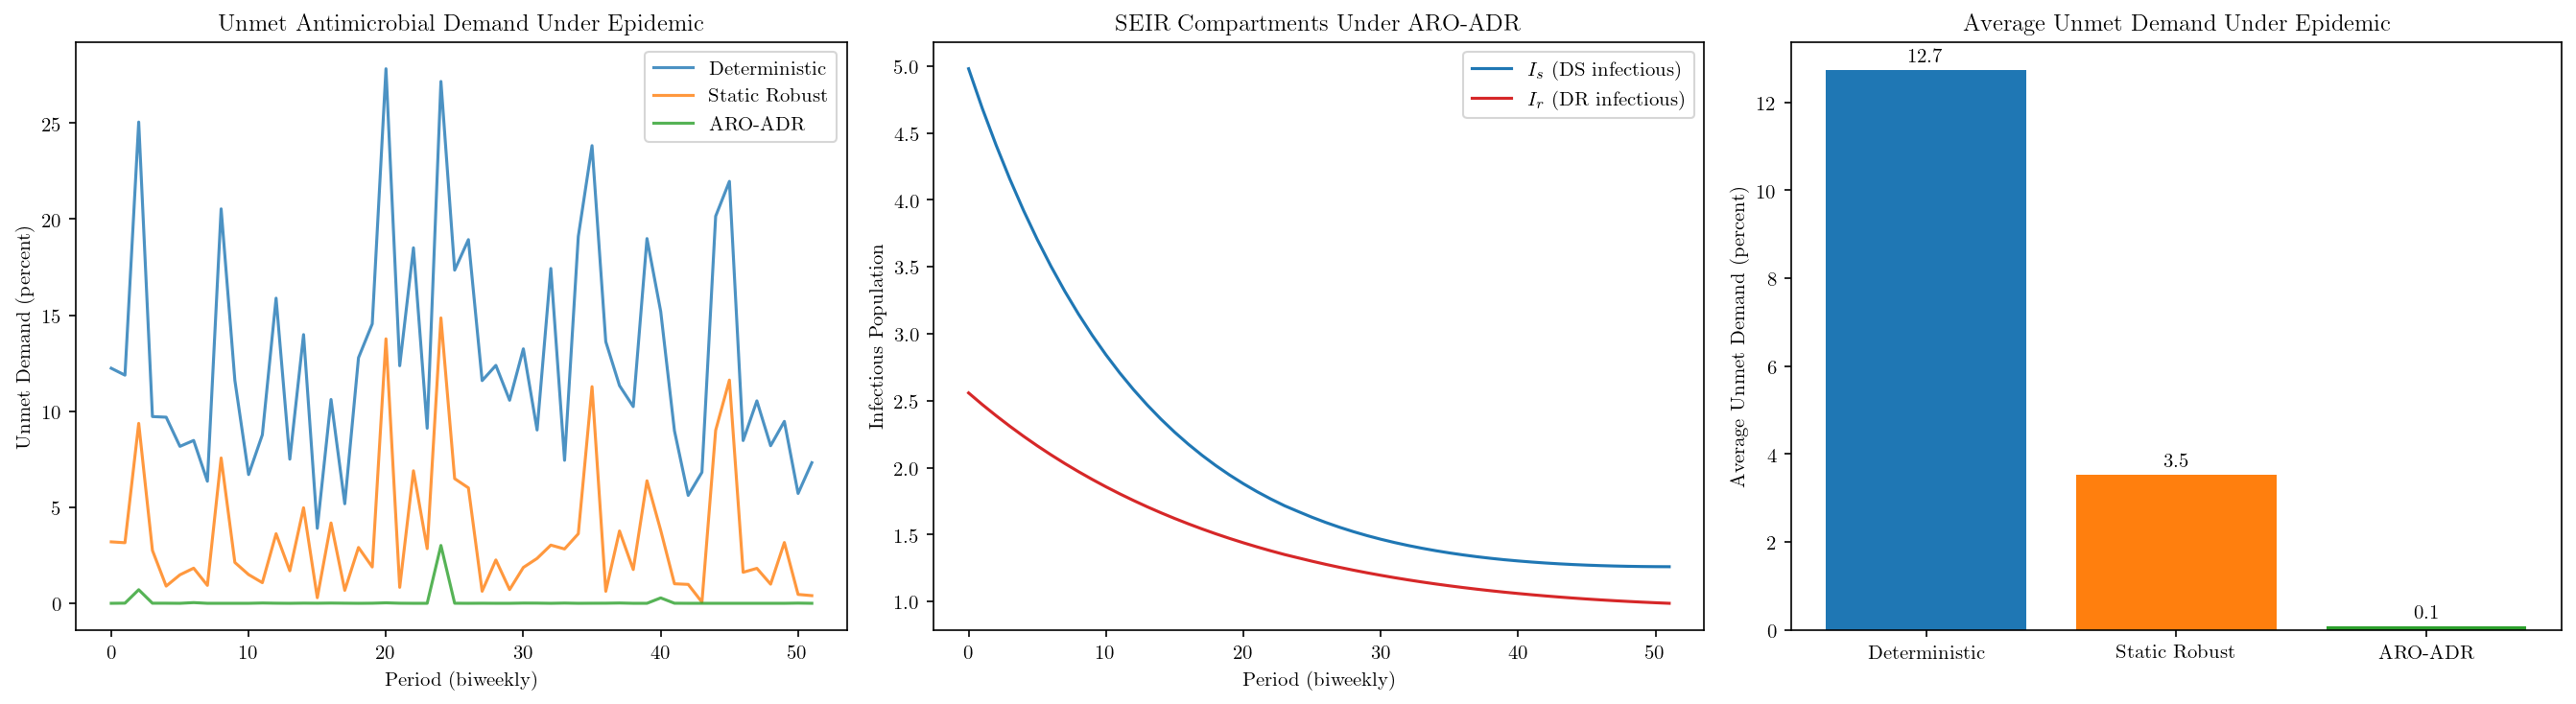
\includegraphics[width=1\linewidth]{epidemic_gaborone_results.png}
    \caption{Epidemic demand resilience results at Princess Marina Hospital under three allocation policies over a two-year simulation horizon (T=52 biweekly periods). Left: unmet antimicrobial demand over time. Centre: SEIR compartment trajectories under ARO-ADR, showing DS and DR infectious populations declining under adequate drug supply. Right: average unmet demand by policy.}
    \label{fig:epi_results}
\end{figure}

\begin{figure}[htbp]
    \centering
    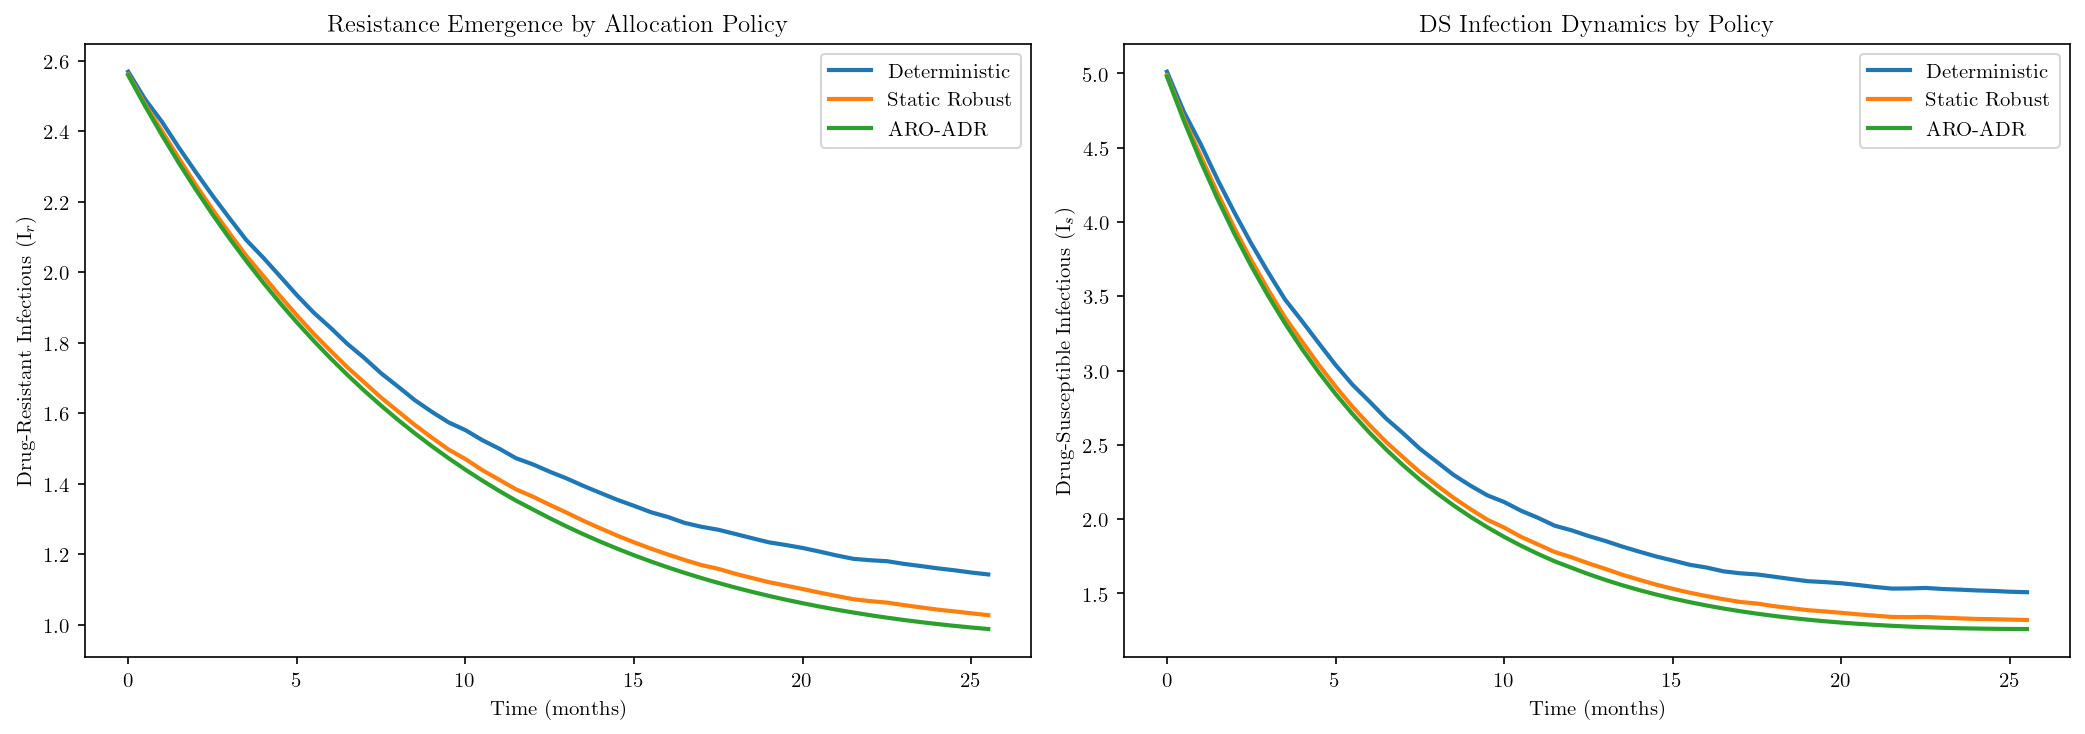
\includegraphics[width=\textwidth]{resistance_emergence_comparison.png}
    \caption{Resistance emergence and DS infection dynamics at Princess Marina Hospital under three allocation policies over a two-year simulation horizon (T=52 biweekly periods). Left: drug-resistant infectious population $I_r$ over time. Right: drug-susceptible infectious population $I_s$ over time. The deterministic policy, which sustains average cephalosporin shortages of 12.7\%, exhibits slower clearance of both strains relative to the robust policies, with final values of $I_r = 1.14$ and $I_s = 1.51$ compared to $I_r = 1.03$, $I_s = 1.32$ under static robust and $I_r = 0.99$, $I_s = 1.26$ under ARO-ADR. The two robust policies are nearly indistinguishable, consistent with the weak resistance amplification channel ($\rho = 0.07$) and the two-year simulation window.} \label{fig:epi_resistance}
\end{figure}

\subsubsection{Results}

Table~\ref{tab:epi_results} summarizes the performance of the three allocation policies under epidemic-driven demand at Princess Marina Hospital over a two-year simulation horizon. The policy ordering mirrors the national trial: ARO-ADR achieves the lowest average unmet demand (0.1\%), followed by static robust (3.5\%) and deterministic (12.7\%), as shown in the bar chart of Figure~\ref{fig:epi_results}. The unmet demand time series in the left panel of Figure~\ref{fig:epi_results} confirms that this ordering is stable across all 52 biweekly periods, with ARO-ADR maintaining near-zero shortages even during epidemic demand spikes that drive the deterministic policy to shortfalls exceeding 25\%.

The SEIR compartment trajectories under ARO-ADR are shown in the centre panel of Figure~\ref{fig:epi_results}. Both the DS infectious population $I_s$ and the DR infectious population $I_r$ decline over the simulation horizon, reflecting the combined effect of treatment and natural recovery under adequate drug supply. The system operates below the epidemic threshold at the hospital scale, consistent with a setting in which active treatment is maintained throughout. The declining trajectories confirm that the epidemic demand generated by the SEIR layer is not driven by uncontrolled outbreak growth but by the resolution of an initial infectious burden under treatment, with demand falling as the infectious population clears.

The resistance dynamics across policies are shown in Figure~\ref{fig:epi_resistance}. Supply chain performance has a measurable effect on the trajectory of both infectious compartments over the two-year horizon. Under the deterministic policy, chronic cephalosporin shortages suppress the DS treatment rate $\tau_s$, slowing clearance of $I_s$ and sustaining the resistance amplification pathway $\rho \tau_s I_s$ at elevated levels for longer. By contrast, the two robust policies, which maintain near-full supply throughout, clear both strains more rapidly. At the end of the simulation horizon, the deterministic policy yields final compartment values of $I_s = 1.51$ and $I_r = 1.14$, compared to $I_s = 1.32$, $I_r = 1.03$ under static robust and $I_s = 1.26$, $I_r = 0.99$ under ARO-ADR. The gap between the deterministic policy and the two robust policies is visible from approximately month 5 onward and widens steadily, reflecting the compounding effect of repeated supply shortfalls on both strain trajectories.

Static robust and ARO-ADR produce nearly indistinguishable resistance trajectories despite their unmet demand rates differing by a factor of approximately 44 (3.5\% versus 0.1\%). This is consistent with the parameter regime: at $\rho = 0.07$, the resistance amplification channel is weak enough that the marginal difference in supply between the two robust policies does not produce a detectable separation within a two-year window. A longer simulation horizon or a higher amplification probability would be required to discriminate between them on resistance grounds.

The final DR fraction is 43.1\%, 43.7\%, and 43.9\% for the deterministic, static robust, and ARO-ADR policies respectively. This ordering is counterintuitive: the policy with the highest cephalosporin supply produces the highest DR fraction in the short run, because higher $\tau_s$ increases the rate at which DS-infectious individuals pass through the amplification pathway even as it accelerates their clearance. This reflects a well-documented tension in AMR modeling: treatment is simultaneously the mechanism of recovery and the source of resistance amplification \cite{kd20}. The absolute difference across policies is small (0.8 percentage points), and the resistance-reducing effect of faster DS clearance under robust policies is expected to dominate over longer time horizons than those examined here.

These results present a nuanced picture of the relationship between supply chain performance and resistance outcomes. On the one hand, the absolute drug-resistant infectious burden $I_r$ is lower under better-supplied policies: the deterministic policy ends with $I_r = 1.14$ compared to $I_r = 1.03$ under static robust and $I_r = 0.99$ under ARO-ADR, reflecting faster overall clearance of the infectious burden when treatment is reliably maintained. On the other hand, the DR fraction is marginally higher under ARO-ADR (43.9\%) than under the deterministic policy (43.1\%), because higher cephalosporin availability raises $\tau_s$, increasing the rate at which DS-infectious individuals pass through the amplification pathway $\rho \tau_s I_s$ even as it accelerates their clearance. This reflects a well-documented tension in AMR modeling: treatment is simultaneously the mechanism of recovery and the source of resistance amplification \cite{kd20}. The net effect over a two-year horizon favors better-supplied policies on absolute burden but not on strain composition. Over longer horizons, the resistance-reducing effect of faster DS clearance would be expected to dominate, closing this gap.

\section{Discussion}

The results across both the Gaborone proof-of-concept trial and the national simulation confirm the central hypothesis motivating this framework: that adaptive, uncertainty-aware allocation policies substantially outperform static and deterministic approaches in resource-constrained pharmaceutical distribution settings. The ARO-ADR policy reduces average unmet antimicrobial demand to approximately 1.9\%, against 3.6\% for static robust and 13\% for the deterministic baseline, while incurring only a 0.9\% procurement cost premium over static robust. The asymmetry is notable: a marginal increase in procurement expenditure yields a disproportionate reduction in unmet demand, reflecting the core value of affine recourse rules in allowing shipment decisions to respond to realized demand deviations rather than committing to a fixed plan \cite{yanikoglu2018aro}.

A distinguishing feature of the framework is its computational tractability at national scale. The dualization approach described in Section 4.5.2 converts the inner maximization induced by demand uncertainty into a finite collection of linear constraints, yielding a single-level mixed-integer program that remains solvable across a network of 631 facilities and 18 districts. This is a non-trivial property: naive robust formulations that retain the bilevel structure quickly become intractable at this scale, and the ability to solve the reformulated problem within practical time limits is a prerequisite for operational deployment within existing replenishment cycles. The district-level decomposition further contributes to tractability by replacing a single national MIP with 18 independent district-level problems, reducing solve complexity substantially while preserving the allocation integrity of each district's network.

The district decomposition is not only a computational device but also a deliberate equity-preserving design choice. A fully centralized national formulation would allow the optimizer to concentrate allocations toward high-demand urban facilities at the expense of rural health posts, since a cost-minimizing solver naturally favors routes serving large nearby populations. Solving districts independently ensures that each district receives dedicated optimization attention regardless of its population size or geographic accessibility. The results bear this out: under ARO-ADR, the geographic distribution of unmet demand is notably uniform across districts, whereas the deterministic policy concentrates shortfalls in high-demand urban areas. The procurement cost premium of robust policies is similarly distributed evenly across districts, suggesting that the hedging cost does not fall disproportionately on any single part of the network.

The performance gains demonstrated here are also consistent with, and in some respects exceed, what has been achieved through digital logistics interventions in comparable settings \cite{mwencha2016}. The ARO-ADR policy reduces average unmet demand by approximately 11 percentage points relative to the deterministic baseline across the national simulation, without requiring any change to the underlying data collection infrastructure. This comparison is necessarily approximate: other studies have reflected real-world implementation with all its attendant frictions, while the present results are largely simulation-based. Nevertheless, it suggests that optimization-based allocation, layered on top of even modest improvements in data visibility, could yield population-level service gains of a magnitude that has proven achievable in practice.

The seasonality and SEIR extensions confirm that the policy ordering is robust to non-stationary demand and epidemic forcing respectively, though the SEIR results surface a theoretically coherent tension: higher drug availability under ARO-ADR leads to marginally greater short-run resistance amplification because higher treatment rates increase the rate at which drug-susceptible individuals pass through the resistance amplification pathway \cite{kd20}. The supply chain benefits of the framework should therefore be evaluated primarily on service coverage grounds rather than resistance outcomes over short horizons, with the resistance-reducing effect of faster susceptible strain clearance expected to dominate only over longer time windows than those examined here.

\subsection{Parameter Assumptions}

The framework developed in this thesis is designed as a decision-support platform rather than as a definitive forecasting model of antimicrobial demand in Botswana. Its primary objective is to provide a flexible structure within which the Government of Botswana may input updated administrative and epidemiological data and evaluate allocation strategies under alternative scenarios. As such, several simplifying assumptions are imposed to ensure transparency and tractability.

Demand estimation relies on a generalized linear model (GLM) trained on available facility-level data. Because the point prevalence survey used for calibration covers inpatient antimicrobial use only and is drawn from a single district, the resulting demand estimates capture a partial slice of true facility-level need. Outpatient consumption, community-level dispensing, and informal procurement channels are not reflected. The GLM additionally replaces a number of facility-level demand estimates with zero due to low predicted counts in sparsely populated catchments; in practice, Central Medical Stores consumption records at the stock-keeping unit level would not exhibit this truncation, since even low-volume facilities generate nonzero dispensing records over any planning horizon. The demand estimates should therefore be understood as lower bounds on true facility need rather than complete forecasts. The objective is not to extract a precise function of demand from incomplete data, but to produce reasonable estimates sufficient to test the optimization framework under conditions of limited data visibility that are realistic for the settings this model targets. The core optimization structure requires no modification to accommodate richer demand inputs as they become available.

Spatial relationships across facilities are incorporated only through covariates and geographic distance measures. The framework does not impose a fully specified spatial transmission mechanism nor assume deterministic spillovers between neighboring locations. Instead, epidemiological uncertainty is introduced through stylized compartmental dynamics that generate scenario-based shocks. These dynamics are intended to test the system's resilience under alternative outbreak trajectories rather than to replicate the full heterogeneity of contact networks or resistance evolution. Several biological parameters in the two-strain SEIR layer, including progression rates, recovery rates, and the resistance amplification probability, are drawn from \cite{kd20} as published values for a tractable two-strain bacterial infection model, without claiming direct transferability to Botswana's specific epidemiological context.

The supply chain component assumes fixed transportation costs, known routing distances, and an exogenously specified budget constraint within each decision epoch. In practice, governments may engage in borrowing, emergency procurement, or donor-supported scale-up that relaxes short-run fiscal limits. The budget assumption therefore represents a policy scenario rather than a claim about institutional rigidity. Alternative fiscal regimes, such as high initial capitalization with dynamic replenishment, can be incorporated within the same optimization structure.

More broadly, the model abstracts from measurement error and administrative frictions in stock reporting. These features are not ignored conceptually but are outside the present scope given data constraints. The framework is intentionally modular so that improved administrative inputs, refined epidemiological models, or alternative statistical estimators may be integrated without altering the core optimization structure.

Accordingly, quantitative outputs should be interpreted as scenario-based simulations conditional on maintained assumptions. The principal contribution lies in demonstrating that the system can learn from observed data inputs, update demand projections, and optimize allocation decisions under epidemiological uncertainty. The framework is therefore best understood as a scalable policy and data-based tool capable of refinement as institutional data infrastructure improves.

\subsection{Future Work}

Several directions present themselves as natural extensions of the present work. The most immediate limitation is one of data availability. The demand model relies on population-weighted facility assignments, district-level admissions estimates, and a GLM-derived drug class distribution, all of which would be approximations of demand at the facility-level. As ordering records become more detailed towards both the facility level and drugs of interest, the baseline means $\mu_{n,k}$ and dispersion parameter $\kappa$ can be used to better construct the uncertainty set. Improving the granularity of stock management data, particularly at clinic and health post level, is therefore a goal that can further strengthen this framework in operational use.

A second direction concerns the feedback between consumption patterns and antimicrobial resistance. The present model treats demand for each drug class as a function of population and infection prevalence, but does not account for the secular trend toward second-line agents as resistance to first-line drugs accumulates. Machine learning methods have recently been applied to predict future resistance prevalence from longitudinal surveillance data at the hospital level \cite{vihta2024}, and integrating such predictions into the uncertainty set would allow the model to anticipate demand shifts driven by resistance dynamics rather than treating $\mu_{n,k}$ as stationary over multi-year planning horizons. This is particularly relevant for the aminoglycoside, quinolone, and lincosamide classes considered in the seasonal analysis, where growing MDR-TB and XDR-TB burden in Southern Africa is likely to place increasing pressure on second-line procurement.

Third, the model currently assumes that the CMS can procure any quantity at a known unit cost with no supply-side uncertainty. In practice, procurement lead times, supplier reliability, and international price volatility for second-line TB drugs sourced through global mechanisms introduce uncertainty on the supply side that is at least as consequential as demand uncertainty. Extending the ARO-ADR framework to jointly optimize upstream procurement and downstream distribution under both supply and demand uncertainty represents a natural multi-echelon generalization of the present work.

Finally, the model has been evaluated entirely in simulation. The present work has been conducted in collaboration with Botswana's Ministry of Health, which provided the aggregate dispensing and facility records that underpin the demand model. Validating the approach against historical stockout records from the Botswana CMS, and piloting the policy in a small number of DHMTs prior to any national rollout, would provide the empirical grounding necessary for policy adoption. The principal remaining barrier is not institutional but informational: as noted above, the records used in this study do not yet capture dispensing quantities disaggregated by drug class and facility, and closing this gap is the most direct path toward operationalizing the framework. Health supply chain research in LMICs has consistently shown that even well-designed optimization models require corresponding investment in data infrastructure and human capacity to translate model outputs into procurement decisions \cite{duwiejua2025}, and the existence of an institutional partnership with the Ministry of Health places Botswana in a stronger position than most to make that investment.

\section{Global Health Implications}

The optimization framework developed in this thesis is motivated by an operational problem specific to Botswana, but the forces that produced that problem are not specific to Botswana. Unreliable access to essential medicines, fragmented supply chains, and health systems whose financing is structurally exposed to external shocks are defining features of public health in much of sub-Saharan Africa and the broader low- and middle-income world. This chapter situates the thesis within that wider context. It examines the Botswana medical crisis as a regional case study, considers the relationship between antimicrobial prescribing practices and supply chain performance, and discusses the socioeconomic and epidemiological frameworks through which the health consequences of distribution failures are best understood.

\subsection{Botswana Medical Crisis and Regional Applicability}

In August 2025, Botswana declared a national public health emergency after widespread medicine shortages left clinics without essential drugs across the country \cite{reut25}. The crisis was precipitated by a confluence of fiscal contraction, reduced foreign aid, and longstanding procurement fragilities, and it drew international attention to a vulnerability that is far from unique to Botswana. Across sub-Saharan Africa, most countries import between 70\% and 90\% of their pharmaceutical supply, leaving health systems structurally exposed to currency shocks, donor volatility, and global supply disruptions \cite{adebisi2022}. In this respect, Botswana's emergency is better understood as a regional warning than as a country-specific failure.

The broader literature on pharmaceutical supply chain fragility in Africa identifies a consistent set of structural drivers: import dependence, weak inventory management, poor cold chain and storage infrastructure, and fragmented distribution networks that lack digital visibility \cite{olutuase2022}. These conditions are compounded in economies where health financing is tightly coupled to a single commodity revenue stream. When that stream contracts, as occurred in Botswana following the decline of the global diamond market, fiscal adjustment falls disproportionately on recurrent expenditures like drug procurement, precisely because capital commitments and wage bills are harder to reduce in the short term. The result is a predictable but largely unmitigated boom-bust cycle in medicine availability.

Addressing these dynamics requires more than emergency financing. It requires allocation frameworks that are robust to the demand uncertainty and supply volatility that characterize resource-limited health systems. Optimization-based approaches of the kind developed in this thesis are one such tool. However, their replication in other regional settings depends on data infrastructure that is not uniformly available. The present model relies on facility-level geocoding, road-network routing data, and stock-keeping unit consumption records assembled through direct collaboration with government partners. In countries with weaker civil registration systems or less digitized logistics management platforms, these inputs may require substantial preparatory investment before a comparable framework can be deployed. The broader literature on pharmaceutical supply chain fragility in Africa identifies a consistent set of structural drivers: import dependence, weak inventory management, poor cold chain and storage infrastructure, and fragmented distribution networks that lack digital visibility \cite{olutuase2022}. Only eight countries across the entire African continent currently operate pharmaceutical regulatory systems at the WHO's maturity level three or above, and the distribution of health management information systems remains highly uneven \cite{duga2025}. Tanzania's introduction of an electronic logistics system offers a concrete illustration of what is achievable: stockout rates fell from 32\% to 23\% following implementation, suggesting that targeted digital infrastructure investment can meaningfully improve supply chain performance even without a full optimization overlay \cite{mwencha2016}.

The general principle underlying this work, that adaptive and uncertainty-aware allocation substantially outperforms static planning under volatile conditions, does not require rich data to be valid. Even in settings where facility-level consumption records are incomplete, the budgeted uncertainty set structure can be calibrated to coarser district-level aggregates, and the district-level decomposition used in the national trial is already designed with this scalability in mind. The Botswana case thus illustrates both the urgency of the problem this framework addresses and the conditions under which analogous approaches could be progressively adopted across the region as digital health infrastructure matures.

\subsection{Antimicrobial Practices}

Physician behavior sits at the intersection of two opposing pressures in resource-limited health systems: the tendency to overprescribe when diagnostics are unavailable, and the forced interruption of treatment when drugs are not. Both dynamics accelerate antimicrobial resistance, and both are shaped by supply chain conditions.

In the absence of functional microbiology laboratories and point-of-care diagnostic tools, clinicians across sub-Saharan Africa routinely prescribe broad-spectrum antibiotics empirically, without microbiological confirmation of the causative pathogen \cite{ehsan2025}. Scoping reviews of prescribing practice find that the overwhelming majority of healthcare workers prescribe empirically as their default, and that outdated national treatment guidelines lacking local antibiogram data further entrench this pattern \cite{chigome2025}. The result is selection pressure for resistant strains even when individual prescribers are acting in good faith under genuine diagnostic uncertainty.

The opposing problem is equally consequential. When first-line drugs are stocked out, physicians are forced either to withhold treatment entirely or to substitute second-line agents for which patients may be less suitable and which carry greater risks of accelerating resistance \cite{lax13}. But the relationship between stockouts and prescribing behavior is more complicated than simple substitution. Field interviews conducted during site visits for this study revealed that clinicians in district settings sometimes preemptively prescribe second-line agents not because first-line drugs are absent, but because repeated exposure to supply interruptions has led them to anticipate first-line treatment failure. In other words, a history of unreliable availability shapes clinical judgment even when drugs are momentarily in stock, creating a feedback loop in which past distribution failures propagate resistance-accelerating prescribing decisions into the future.

These dynamics together suggest that reliable drug availability and responsible prescribing are complements, not substitutes. Ensuring that first-line antimicrobials are consistently stocked is a necessary condition for stewardship to function: a physician cannot follow guideline-concordant prescribing if the recommended drug is absent, or if prior experience has taught them not to trust that it will remain available. But availability alone is insufficient. If drugs are reliably stocked but prescribed without diagnostic support, administered at incorrect doses, or dispensed for viral presentations, resistance will advance regardless of how well the supply chain performs. Effective antimicrobial governance therefore requires simultaneous investment in distribution infrastructure, diagnostic capacity, and clinical education, with neither dimension treated as a substitute for the other.

\subsection{Measures of Life Lost}

Disability-Adjusted Life Years (DALYs) are the dominant metric for quantifying the burden of disease in global health, aggregating years of life lost to premature mortality and years lived with disability into a single index \cite{murray1994}. Their appeal is practical: they permit comparisons across diseases, populations, and interventions, and they have become the standard currency of cost-effectiveness analysis in low- and middle-income country health policy \cite{voigt2012}.

The optimization framework developed in this thesis includes an unmet demand penalty parameter $\Delta_{n,k}$ that is formally compatible with DALY-based cost weights: one could, in principle, calibrate the penalty to reflect the expected disability-adjusted life years lost per unit of unmet antimicrobial demand at each facility. We deliberately did not frame it this way. The DALY literature carries well-documented concerns that bear directly on this choice. The standard construction applies age-weighting and discounting that embed normative assumptions about the relative value of life years at different ages, assumptions that have been contested on both ethical and empirical grounds \cite{arne99}. The disability weights assigned to infectious disease sequelae are derived largely from expert elicitation in high-income settings and may not reflect the values or lived experience of the populations this model serves \cite{voigt2012}. Applying such weights in Botswana's context risks importing distortions alongside the analytical convenience they offer.

The penalty parameter therefore functions in this thesis as a tuning parameter rather than a welfare measure: it controls the relative weight placed on service coverage versus procurement cost in the objective function, and its value is set to reflect operational priorities rather than claimed as a precise estimate of social harm. This is a more honest use of the construct. It preserves the model's ability to prioritize access without committing to the contested cardinal valuations that a full DALY-based framing would require.

\subsection{Socioeconomic Determinants of Health}

The distribution of antimicrobial access is not random. It follows the contours of poverty, geography, and political economy with a regularity that resists purely technical explanation. Paul Farmer's framework of structural violence offers the most coherent account of this pattern: the social arrangements that determine who falls ill and who receives treatment are not incidental to health systems but constitutive of them \cite{farmer2006}. In his formulation, poverty is not merely a background condition that makes health harder to achieve; it is itself a pathology, one that operates through the denial of access to medicines, diagnostic services, and the infrastructure required to deliver them.

This framing has direct implications for the interpretation of pharmaceutical distribution failures in sub-Saharan Africa. Stockouts at rural health posts, interrupted treatment courses, and the substitution of second-line agents when first-line drugs are unavailable are not primarily the result of poor logistics planning. They are downstream expressions of structural conditions in which health financing is chronically underfunded, procurement systems are starved of fiscal resources, and the populations most dependent on public facilities have the least political leverage to demand improvement. Farmer's critique of cost-effectiveness as the organizing principle of global health resource allocation is particularly apt here: frameworks that accept scarcity as a given and optimize within it risk laundering structural inequality as operational necessity \cite{farmer2004}.

Supply chain optimization, of the kind developed in this thesis, operates necessarily within these structural constraints rather than outside them. It cannot resolve the underlying fiscal conditions that produce stockouts, nor can it substitute for the political commitment required to fund a functional public health system. What it can do is reduce the waste and inefficiency that can compound structural disadvantage at the operational level. In Farmer's terms, it addresses a proximal determinant while the distal causes remain. That is not a reason to dismiss it: as Farmer himself acknowledged, knowing the structural roots of tuberculosis does not relieve the obligation to treat the patient \cite{farmer2006}. Reliable antimicrobial access is both an end in itself and a precondition for the kind of trust in public health institutions that structural reform ultimately requires.

\section{Conclusion}

Antimicrobial supply chains are not peripheral infrastructure. They are a determinant of whether treatment reaches patients, whether resistance emerges, and whether health systems can absorb epidemic shocks. This thesis has attempted to formalize that relationship: by embedding epidemiological feedback into a robust optimization framework, it demonstrates that distribution decisions have measurable consequences for unmet demand, resistance amplification, and population-level health outcomes that static, reactive procurement models systematically fail to anticipate.

The results are specific to Botswana, but the underlying argument is not. In any setting where access rather than innovation is the binding constraint on health, the quality of pharmaceutical logistics is inseparable from the quality of care. Investments in adaptive supply chain management belong alongside investments in clinical capacity, diagnostic infrastructure, and stewardship programs as components of a coherent antimicrobial resistance response. This work is a step toward making that case quantitatively.

\appendix
\appendixpage

\section{Additional Figures}
\begin{figure}[H]
    \centering
    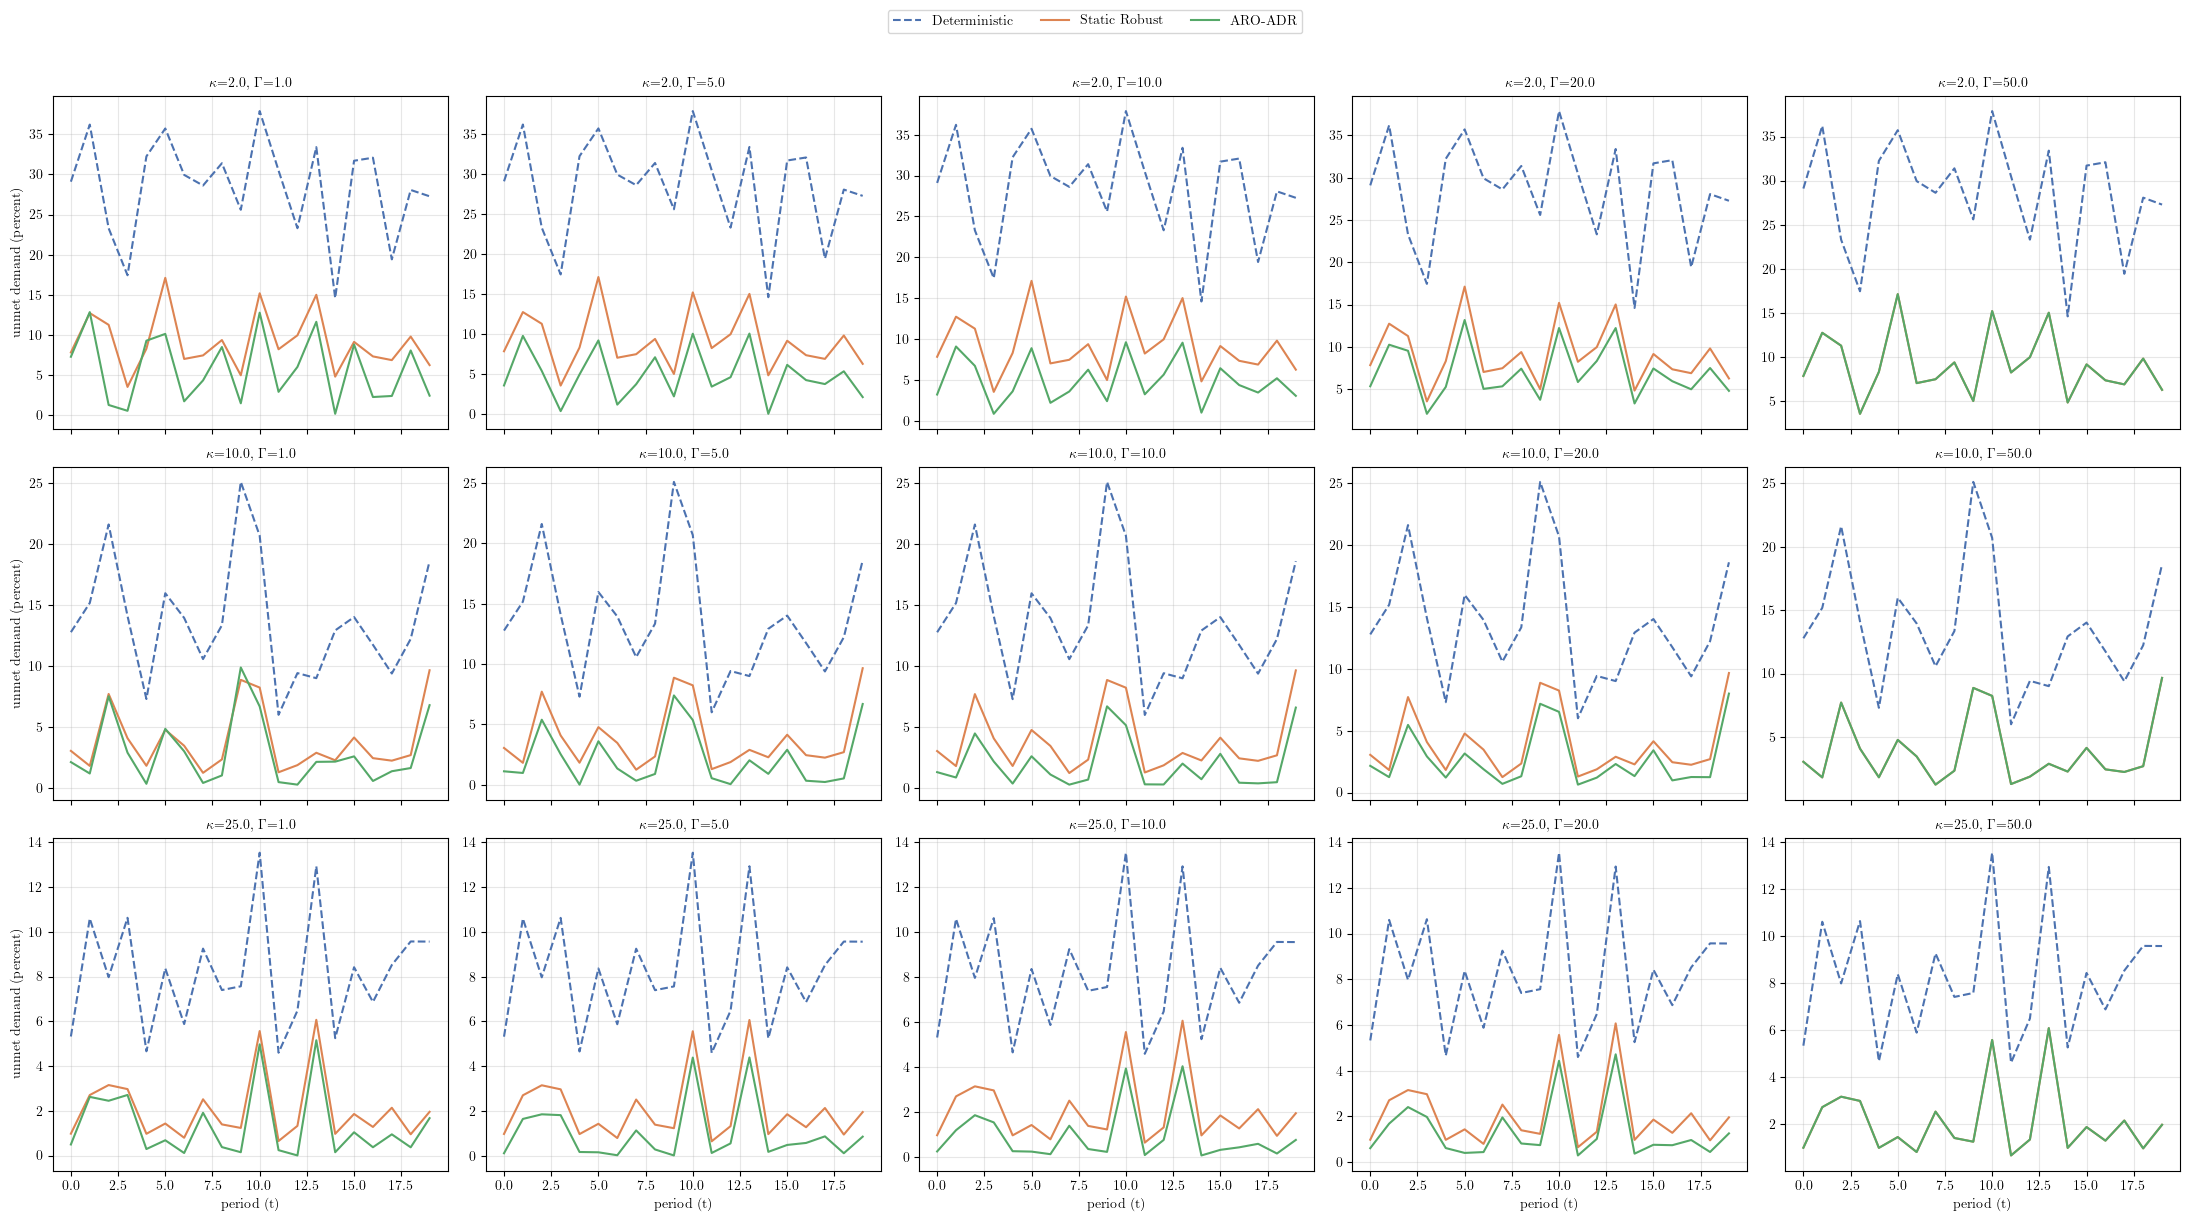
\includegraphics[width=1\linewidth]{gamma_sensitivity.png}
    \caption{Realized unmet demand (\%) across policies for varying uncertainty 
    budget $\Gamma$ (columns) and demand dispersion $\kappa$ (rows). The 
    Deterministic baseline is constant across columns by construction. ARO-ADR 
    converges to Static Robust as $\Gamma$ increases, consistent with the theoretical 
    collapse of the adaptive policy under large uncertainty sets.}
    \label{fig:gamma_sensitivity}
\end{figure}

\begin{figure}[H]
    \centering
    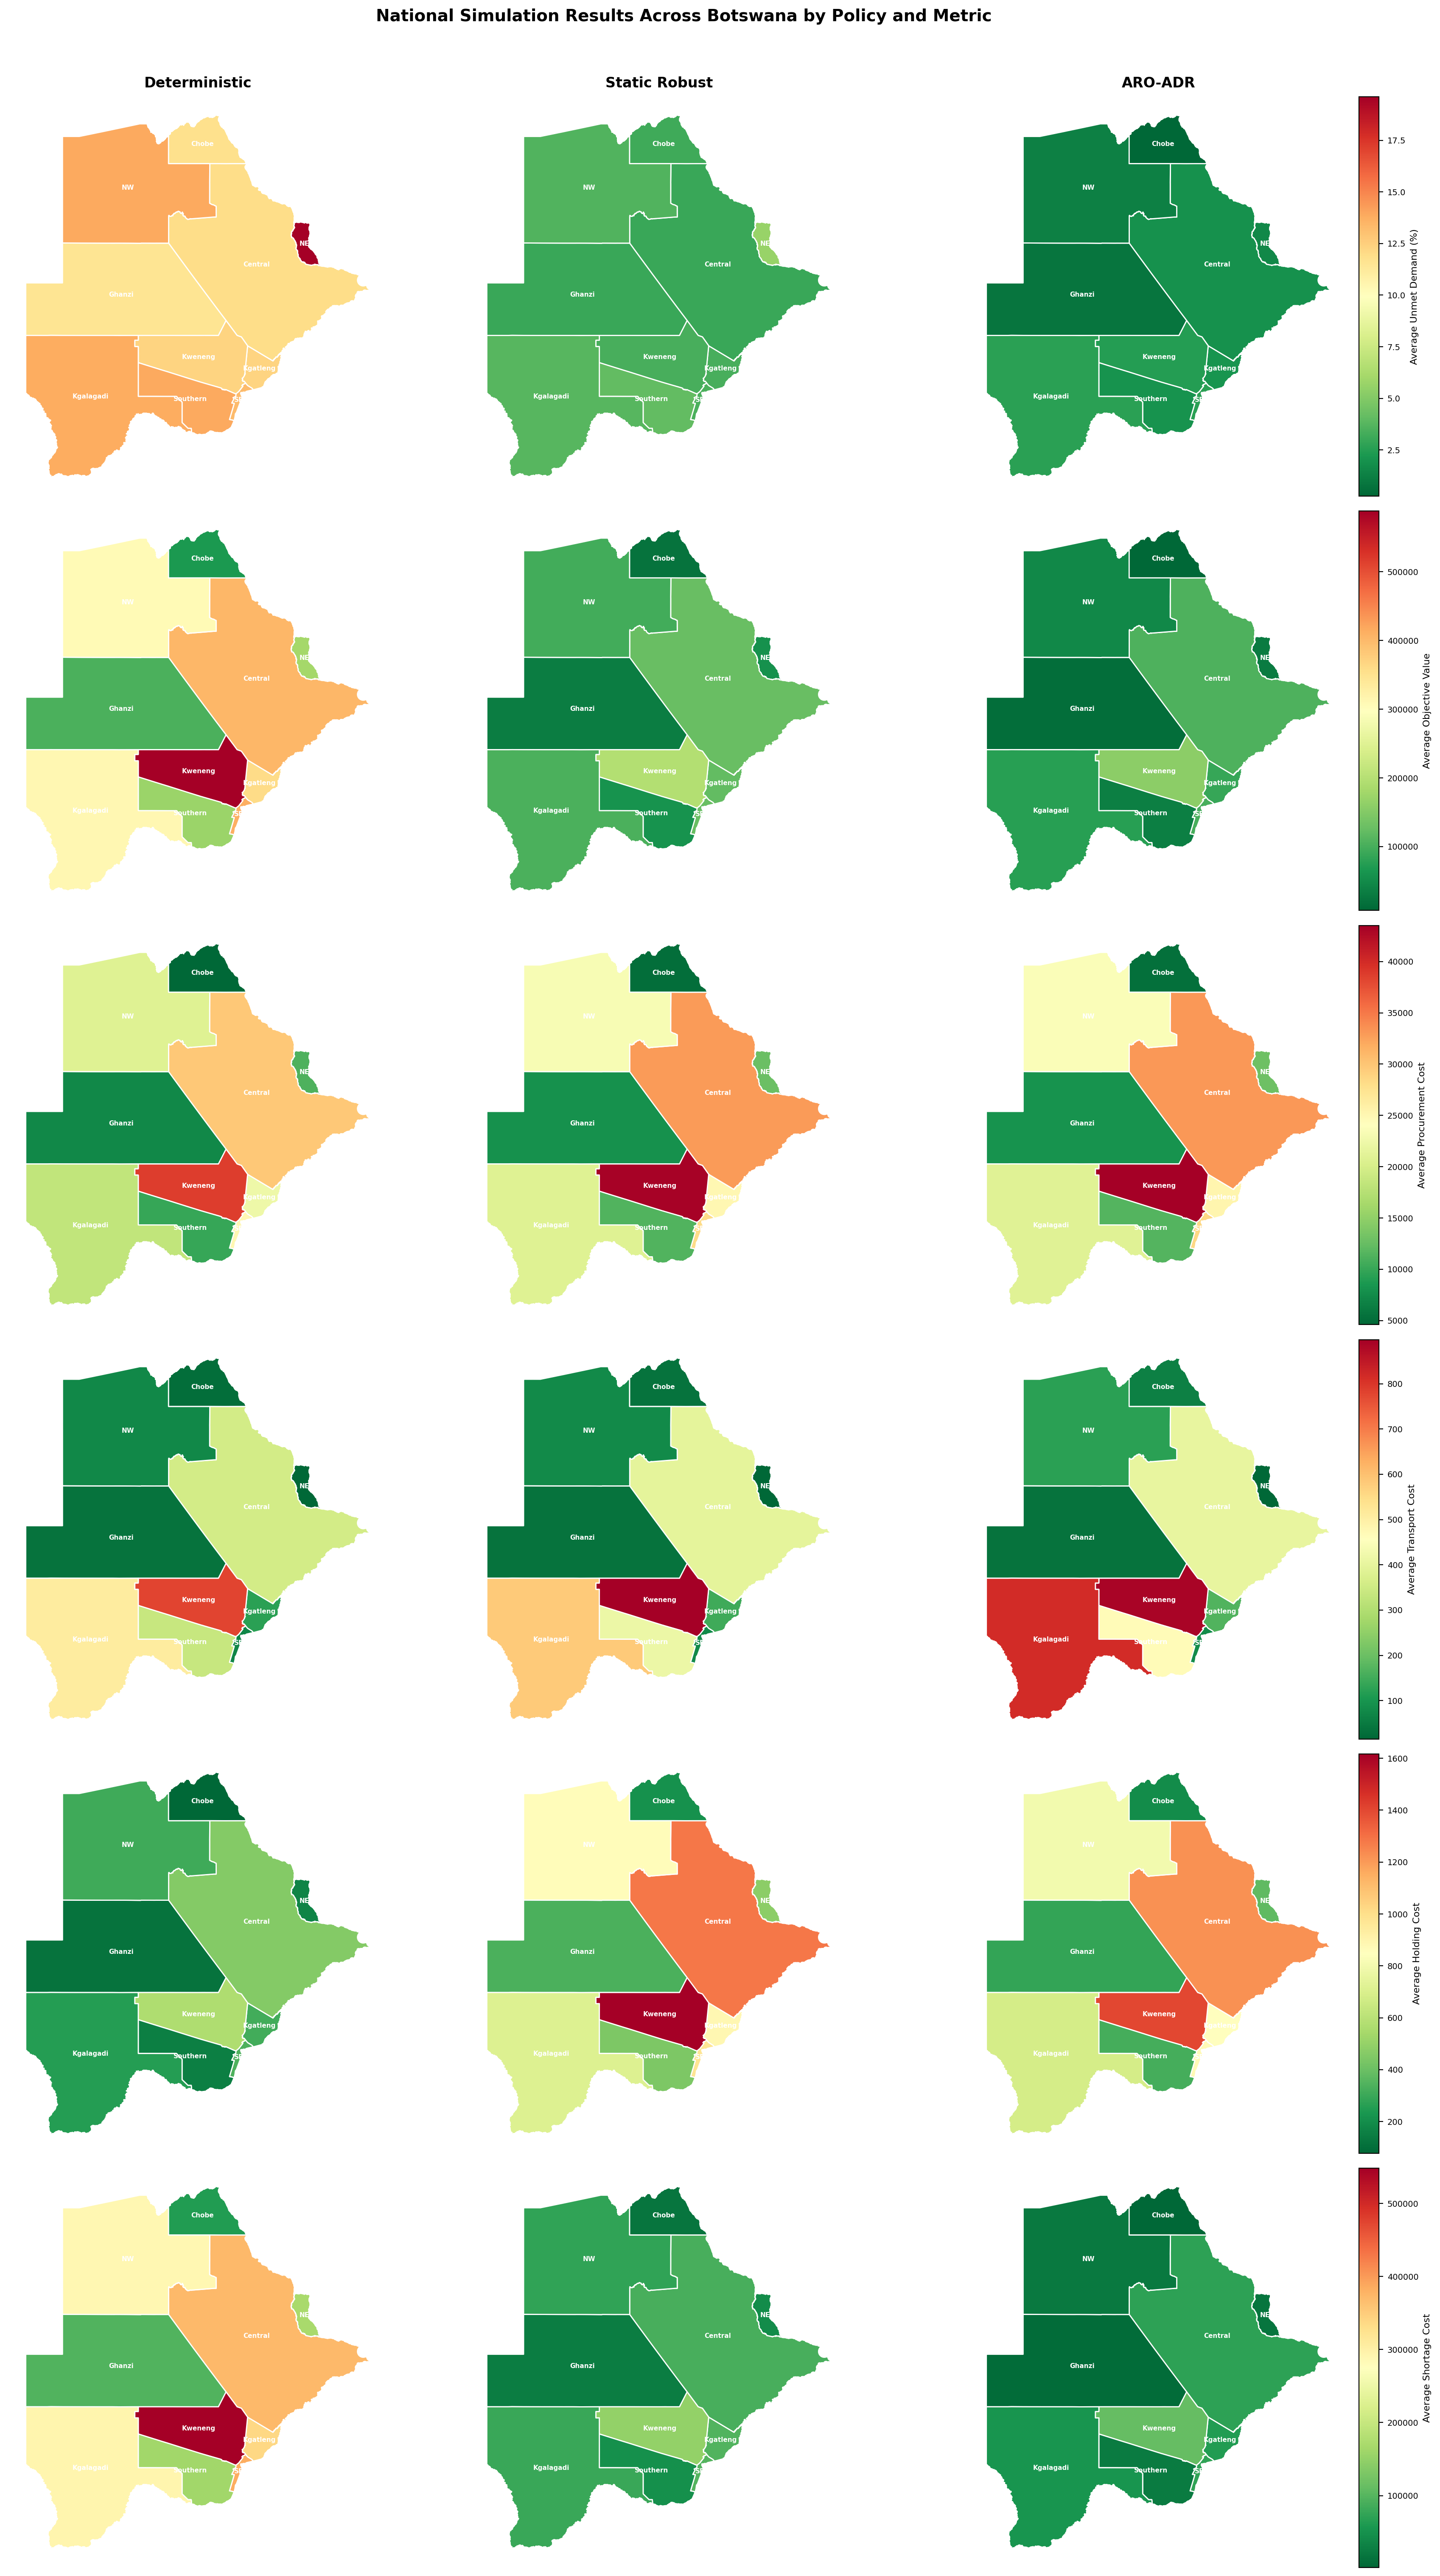
\includegraphics[width=0.7\linewidth]{botswana_appendix_simulation_maps.png}
    \caption{Botswana Simulation Map Results Across All Districts, Indexed by Metric.}\label{fig:botswana_appendix_simulation_maps}
\end{figure}

\begin{figure}[p]
    \centering
    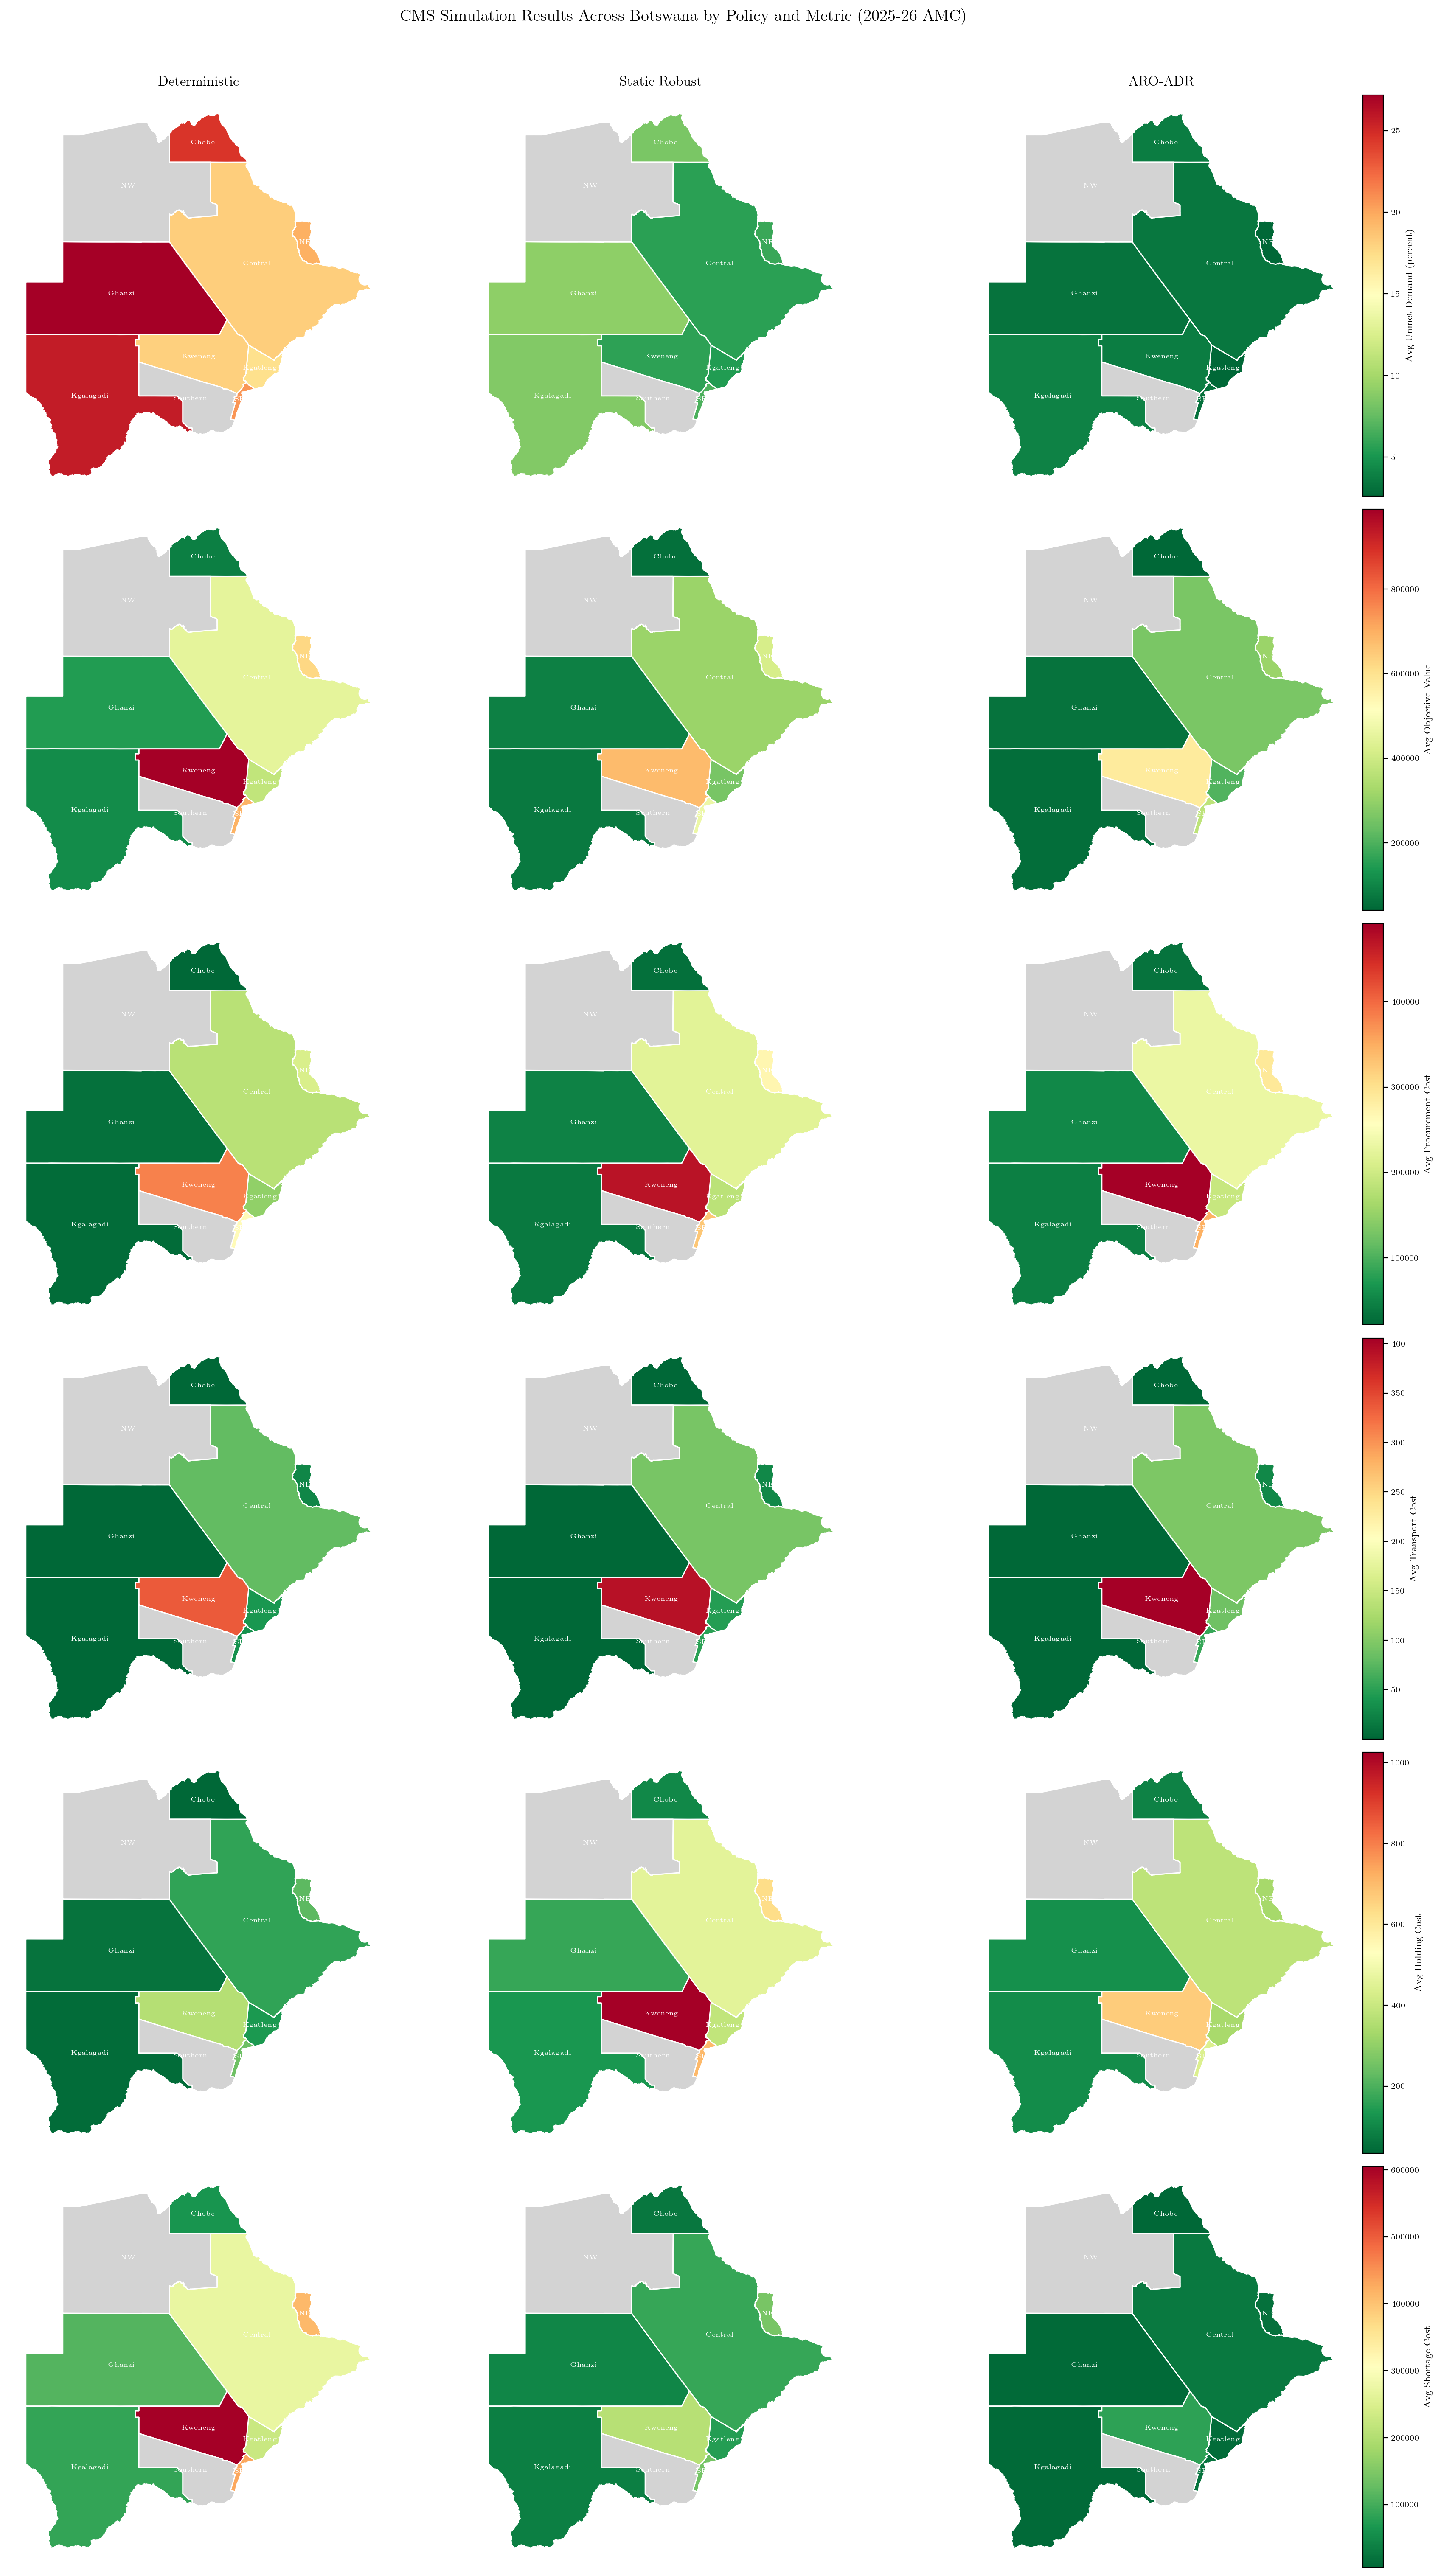
\includegraphics[width=0.65\textwidth]{cms_full_metrics_2526.png}
    \caption{CMS simulation results across Botswana DHMTs by policy and metric, 2025--26 AMC. Rows show average unmet demand, objective value, procurement cost, transport cost, holding cost, and shortage cost. Columns show deterministic, static robust, and ARO-ADR policies.}
    \label{fig:cms_full_2526}
\end{figure}

\begin{figure}[p]
    \centering
    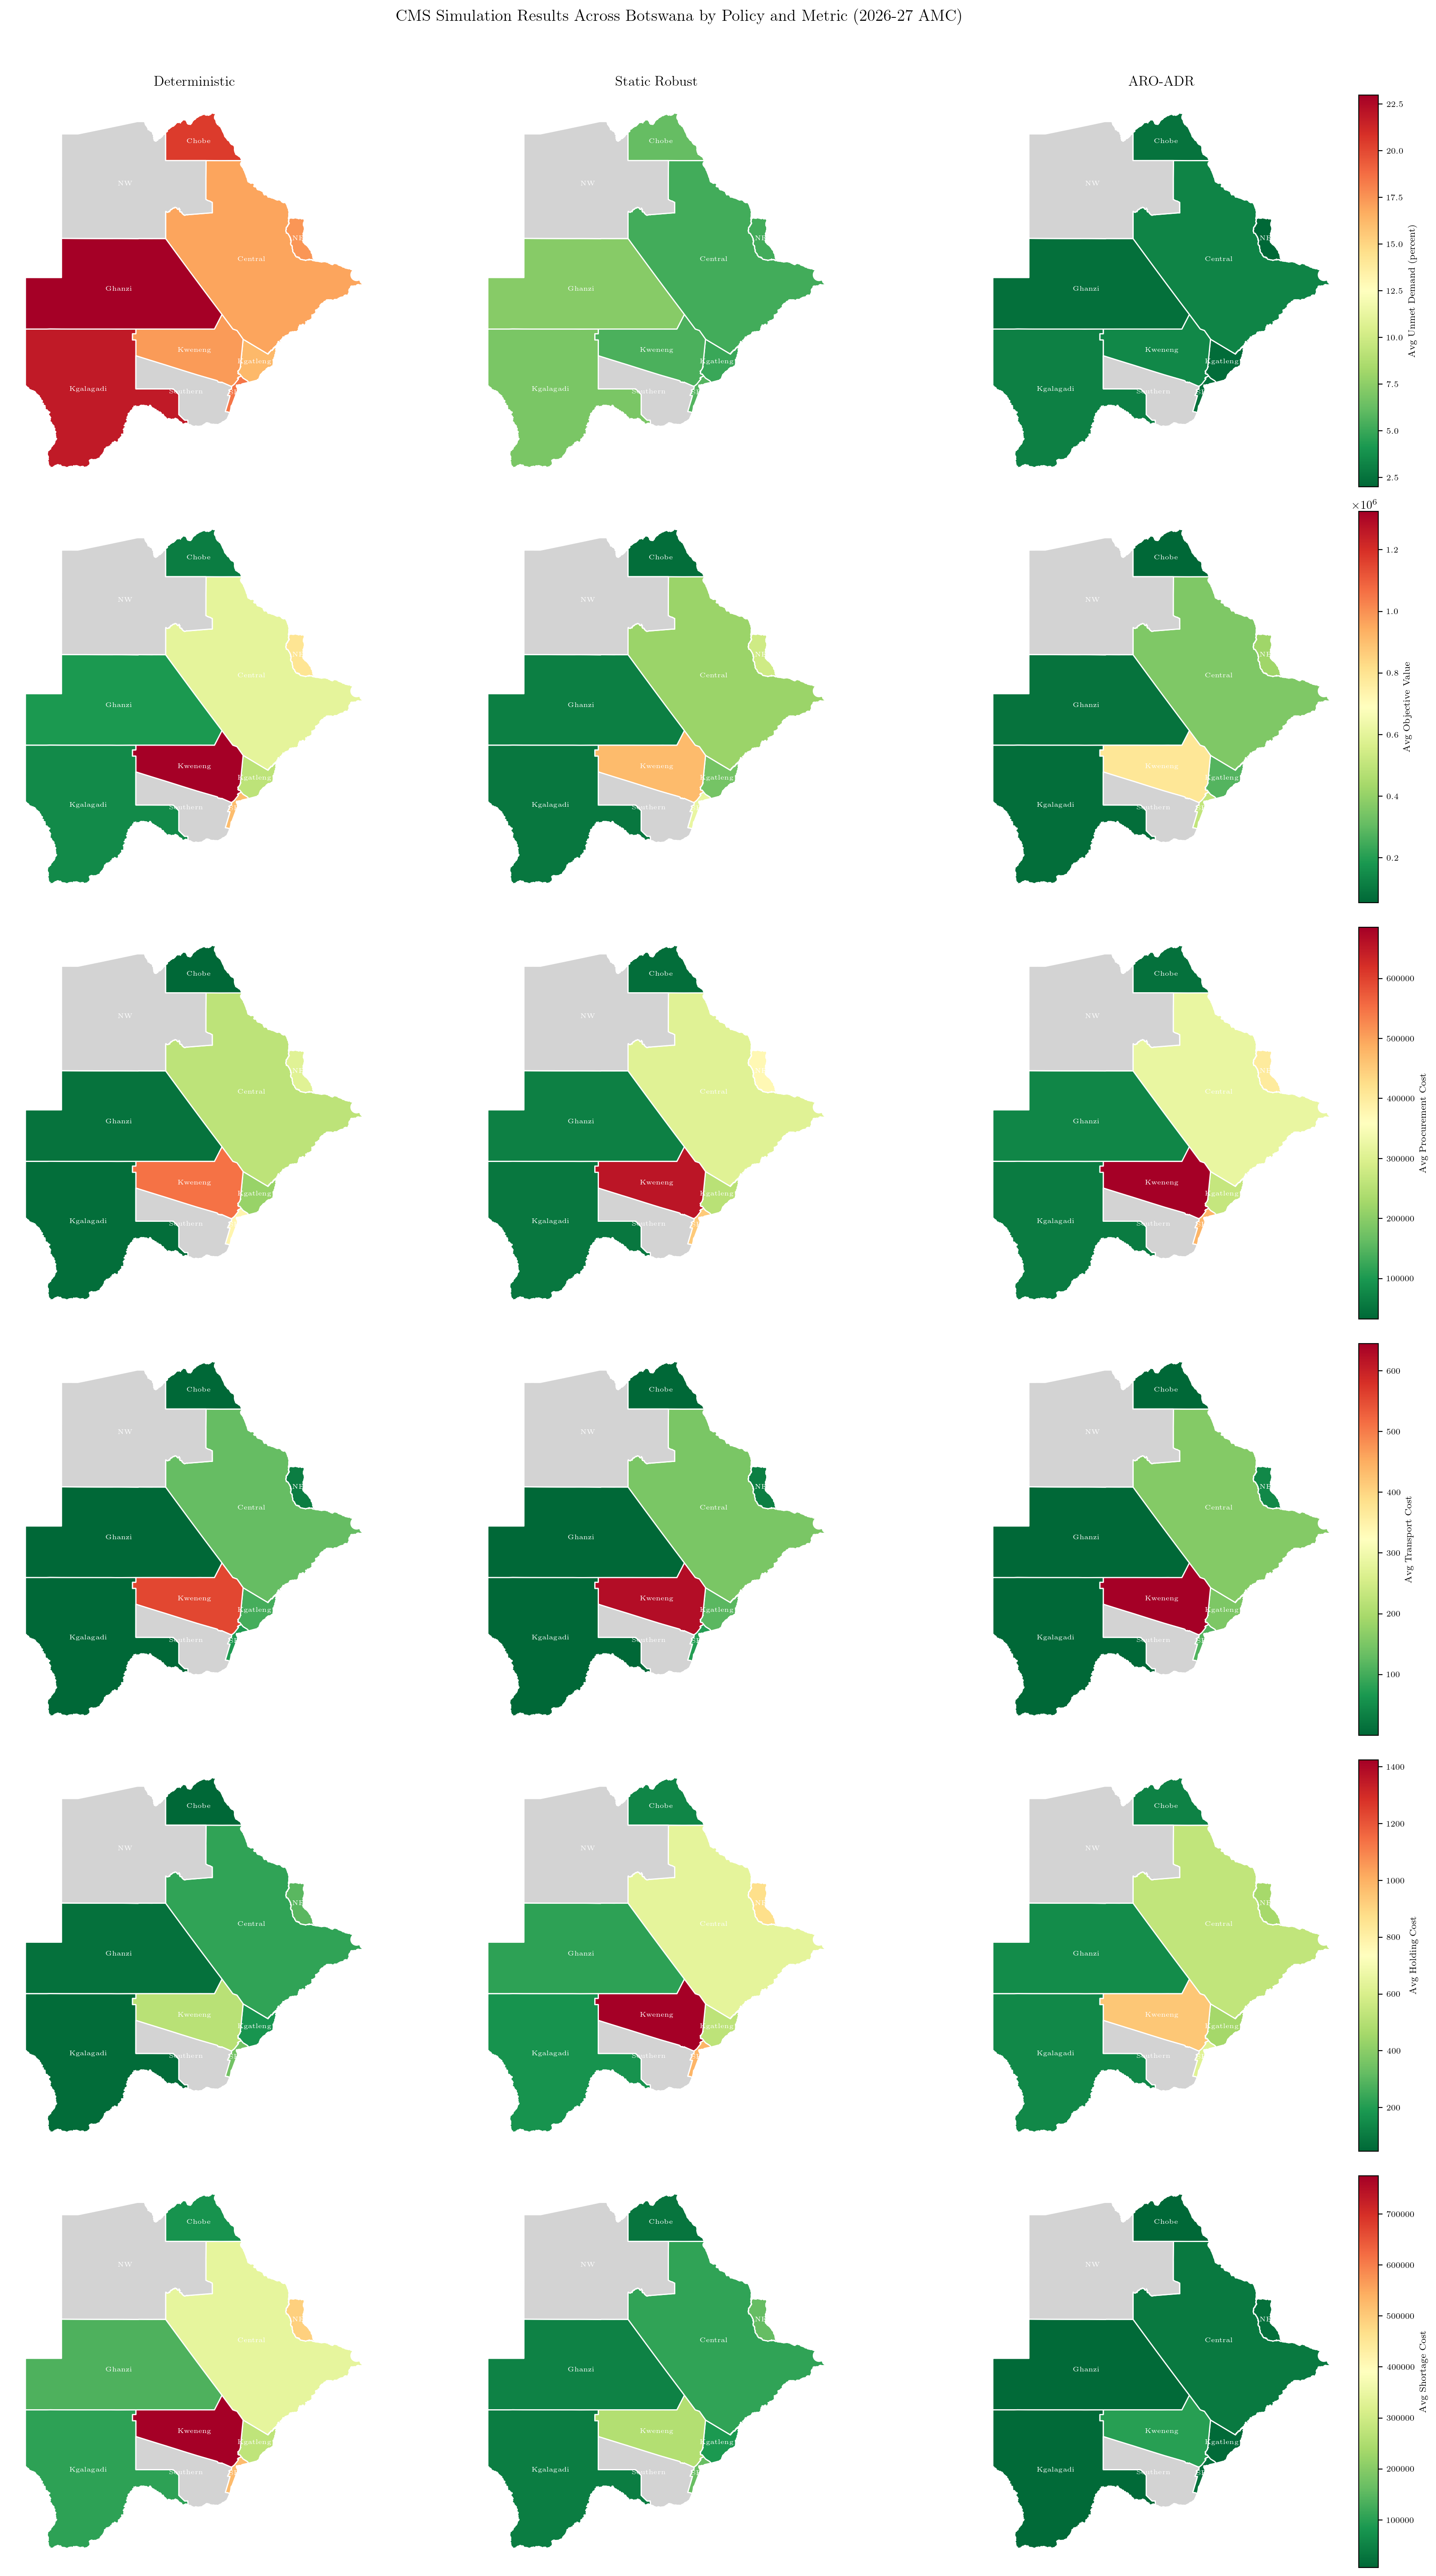
\includegraphics[width=0.65\textwidth]{cms_full_metrics_2627.png}
    \caption{CMS simulation results across Botswana DHMTs by policy and metric, 2026--27 AMC. Layout as in Figure~\ref{fig:cms_full_2526}.}
    \label{fig:cms_full_2627}
\end{figure}

\section{Code}
All code is publicly available and will be consistently updated at 
\href{https://github.com/mistershilai/thesiscode2026}{this GitHub repository}. Note that government data not authorized for release and Google Maps-generated raw data have been withheld for legal reasons.

\section{Dualization Details}
\label{app:dualization}

To obtain a tractable single-level formulation, we dualize the inner
maximization that appears in the robust constraints.

Starting from the inventory balance, we substitute the affine decision rule
\begin{align}
F_{(u,v),k}^{(t)}(\xi^{(t)})
=
\bar F_{(u,v),k}^{(t)}
+
\alpha_{(u,v),k}^{(t)} \xi_{v,k}^{(t)}.
\end{align}
This gives
\begin{align}
I_{n,k}^{(t+1)}
&=
I_{n,k}^{(t)}
+ \sum_{j:(j,n)\in A}
\left(
\bar F_{(j,n),k}^{(t)}
+
\alpha_{(j,n),k}^{(t)} \xi_{n,k}^{(t)}
\right)
\notag\\
&\quad
-
\sum_{r:(n,r)\in A}
\left(
\bar F_{(n,r),k}^{(t)}
+
\alpha_{(n,r),k}^{(t)} \xi_{r,k}^{(t)}
\right)
\notag\\
&\quad
+ \mathbf{1}_{\{n=\mathrm{CMS}\}} q_k^{(t)}
- \bar D_{n,k}^{(t)}
- \xi_{n,k}^{(t)}
+ U_{n,k}^{(t)}.
\end{align}

Collecting the deterministic terms and the terms involving
\(\xi^{(t)}\), the uncertain component in the inventory constraint is
\begin{align}
\left(
\sum_{j:(j,n)\in A} \alpha_{(j,n),k}^{(t)} - 1
\right)\xi_{n,k}^{(t)}
-
\sum_{r:(n,r)\in A} \alpha_{(n,r),k}^{(t)} \xi_{r,k}^{(t)}.
\end{align}

Thus, robust feasibility requires
\begin{align}
\max_{\xi^{(t)} \in \mathcal U^{(k)}}
\Bigg[
\left(
\sum_{j:(j,n)\in A} \alpha_{(j,n),k}^{(t)} - 1
\right)\xi_{n,k}^{(t)}
-
\sum_{r:(n,r)\in A} \alpha_{(n,r),k}^{(t)} \xi_{r,k}^{(t)}
\Bigg]
\le\;&
I_{n,k}^{(t+1)}
-
I_{n,k}^{(t)}
\notag\\
&-
\sum_{j:(j,n)\in A} \bar F_{(j,n),k}^{(t)}
+
\sum_{r:(n,r)\in A} \bar F_{(n,r),k}^{(t)}
\notag\\
&-
\mathbf{1}_{\{n=\mathrm{CMS}\}} q_k^{(t)}
+
\bar D_{n,k}^{(t)}
-
U_{n,k}^{(t)},
\notag\\
&\qquad \forall n \in N,\ k \in K.
\end{align}

\medskip

We now incorporate the shipment-availability constraint. Substituting
the affine decision rule yields
\begin{align}
\sum_{m:(n,m)\in A}
\left(
\bar F_{(n,m),k}^{(t)} + \alpha_{(n,m),k}^{(t)} \xi_{m,k}^{(t)}
\right)
\le\;&
I_{n,k}^{(t)}
+
\sum_{j:(j,n)\in A}
\left(
\bar F_{(j,n),k}^{(t)} + \alpha_{(j,n),k}^{(t)} \xi_{n,k}^{(t)}
\right)
\notag\\
&+
\mathbf{1}_{\{n=\mathrm{CMS}\}} q_k^{(t)}.
\end{align}

Rearranging, the uncertain component becomes
\begin{align}
\sum_{r:(n,r)\in A} \alpha_{(n,r),k}^{(t)} \xi_{r,k}^{(t)}
-
\left(
\sum_{j:(j,n)\in A} \alpha_{(j,n),k}^{(t)}
\right)\xi_{n,k}^{(t)}.
\end{align}

Thus, robust feasibility additionally requires
\begin{align}
\max_{\xi^{(t)} \in \mathcal U^{(k)}}
\Bigg[
\sum_{r:(n,r)\in A} \alpha_{(n,r),k}^{(t)} \xi_{r,k}^{(t)}
-
\left(
\sum_{j:(j,n)\in A} \alpha_{(j,n),k}^{(t)}
\right)\xi_{n,k}^{(t)}
\Bigg]
\le\;&
I_{n,k}^{(t)}
+
\sum_{j:(j,n)\in A} \bar F_{(j,n),k}^{(t)}
\notag\\
&+
\mathbf{1}_{\{n=\mathrm{CMS}\}} q_k^{(t)}
-
\sum_{r:(n,r)\in A} \bar F_{(n,r),k}^{(t)},
\notag\\
&\qquad \forall n \in N,\ k \in K.
\end{align}

\medskip

We now consider the arc-capacity constraint. Substituting the affine
decision rule into
\begin{align}
\sum_{k\in K} F_{(i,j),k}^{(t)}(\xi^{(t)})
\le
\mathrm{cap}\cdot \lambda_{(i,j)}^{(t)},
\end{align}
gives
\begin{align}
\sum_{k\in K}
\left(
\bar F_{(i,j),k}^{(t)}
+
\alpha_{(i,j),k}^{(t)} \xi_{j,k}^{(t)}
\right)
\le
\mathrm{cap}\cdot \lambda_{(i,j)}^{(t)}.
\end{align}

Rearranging, the uncertain component is
\begin{align}
\sum_{k\in K}
\alpha_{(i,j),k}^{(t)} \xi_{j,k}^{(t)}.
\end{align}

Thus, robust feasibility requires
\begin{align}
\max_{\xi^{(t)} \in \mathcal U^{(t)}}
\sum_{k\in K}
\alpha_{(i,j),k}^{(t)} \xi_{j,k}^{(t)}
\le
\mathrm{cap}\cdot \lambda_{(i,j)}^{(t)}
-
\sum_{k\in K} \bar F_{(i,j),k}^{(t)},
\qquad \forall (i,j)\in A.
\end{align}

\medskip

Substituting the Bertsimas--Sim representation
\begin{align}
\xi_{r,k}^{(t)} =
\sigma_{r,k}^{(t)}
\left(
z_{r,k}^{+(t)} - z_{r,k}^{-(t)}
\right),
\end{align}
with
\begin{align}
0 \le z_{r,k}^{+(t)} \le 1,\quad
0 \le z_{r,k}^{-(t)} \le 1,\quad
\sum_{r \in N} \left( z_{r,k}^{+(t)} + z_{r,k}^{-(t)} \right) \le \Gamma,
\end{align}
yields linear programs for all constraints.

Dualizing, we obtain dual variables
\(\theta_{n,k}^{(t)}, \pi^+_{n,k,r}{}^{(t)}, \pi^-_{n,k,r}{}^{(t)}\),
\(\tilde{\theta}_{n,k}^{(t)}, \tilde{\pi}^+_{n,k,r}{}^{(t)}, \tilde{\pi}^-_{n,k,r}{}^{(t)}\),
and
\(\eta_{(i,j)}^{(t)}, \rho^+_{(i,j),k}{}^{(t)}, \rho^-_{(i,j),k}{}^{(t)}\)
for the inventory, shipment, and capacity constraints, respectively.

The resulting single-level conditions are those stated in the main text.

\section{Proofs}

\subsection{Proof of Lemma 1}
\label{B.1}

\begin{proof}
Each term in the full sum of $g$ has the form
\[
h_a(\beta) = N_{r,a}\delta_a \exp(X_{r,a}^\top \beta).
\]
The mapping $\beta \mapsto X_{r,a}^\top \beta$ is linear. 
The exponential function is smooth on $\mathbb{R}$, hence the composition 
$\beta \mapsto \exp(X_{r,a}^\top \beta)$ 
is smooth. 
Multiplication by fixed constants $N_{r,a}$ and $\delta_a$ preserves smoothness.  
Smooth functions are closed under addition, so $g$ is twice-differentiable.

To show Lipschitz continuity on compact $\Theta$, note that the gradient 
\[
\nabla g(\beta)
=
\sum_a 
N_{r,a}X_{r,a}\delta_a\exp(X_{r,a}^\top \beta)
\]
is continuous. 
By the boundedness theorem, a continuous function on a compact set is bounded, so there exists $L > 0$ such that 
$\|\nabla g(\beta)\| \le L$ for all $\beta \in \Theta$.  
By the Mean Value Theorem,
\[
|g(\beta_1) - g(\beta_2)|
\le
L \|\beta_1 - \beta_2\|
\]
for all $\beta_1,\beta_2 \in \Theta$, establishing Lipschitz continuity.
\end{proof}

\subsection{Proof of Theorem 1}
\label{B.2}

\begin{proof}
By Assumptions \ref{assump:glm}--\ref{assump:regularity}, standard maximum likelihood theory for generalized linear models with a log-link and Negative Binomial variance function guarantees that
\[
\hat{\beta}_n \xrightarrow{p} \beta^*
\qquad
\text{as } n \to \infty
\]

Define the deterministic mapping
\[
g(\beta)
=
\sum_a N_{r,a}\delta_a \exp(X_{r,a}^\top \beta).
\]
The function $g:\mathbb{R}^d \to \mathbb{R}$ is smooth and continuous. Since $\hat{\beta}_n \xrightarrow{p} \beta^*$ and $g$ is continuous, the Continuous Mapping Theorem yields
\[
\hat{D}_r
= g(\hat{\beta}_n)
\xrightarrow{p}
g(\beta^*)
= D_r^*.
\]

Thus, the Medical Demand Estimator is consistent.
\end{proof}

\subsection{Proof of Theorem 2}
\label{B.3}

\begin{proof}
Fix a class $i \in \{1,\dots,I\}$. By definition,
\[
D_i = \sum_{j=1}^N Y_{j,i}.
\]

Taking expectations and using linearity of expectation,
\[
\mathbb{E}[D_i]
=
\mathbb{E}\!\left[\sum_{j=1}^N Y_{j,i}\right]
=
\sum_{j=1}^N \mathbb{E}[Y_{j,i}].
\]

Because patient-level vectors $(Y_{j,1},\dots,Y_{j,I})$ are identically distributed across $j$, we have
\[
\mathbb{E}[Y_{j,i}] = \mathbb{E}[Y_{1,i}] \quad \text{for all } j,
\]
so
\[
\mathbb{E}[D_i]
=
N\,\mathbb{E}[Y_{1,i}],
\]
which establishes the stated marginal expectation result.

Next, consider the covariance structure across classes $i \neq k$. We have
\[
\mathrm{Cov}(D_i, D_k)
=
\mathrm{Cov}\!\left(\sum_{j=1}^N Y_{j,i}, \sum_{j=1}^N Y_{j,k}\right)
=
\sum_{j=1}^N \sum_{\ell=1}^N \mathrm{Cov}(Y_{j,i}, Y_{\ell,k}).
\]

By independence across patients, for $j \neq \ell$,
\[
\mathrm{Cov}(Y_{j,i}, Y_{\ell,k}) = 0.
\]
Thus only the $j=\ell$ terms remain:
\[
\mathrm{Cov}(D_i, D_k)
=
\sum_{j=1}^N \mathrm{Cov}(Y_{j,i}, Y_{j,k}).
\]

Using identical distribution across patients,
\[
\mathrm{Cov}(D_i, D_k)
=
N\,\mathrm{Cov}(Y_{1,i}, Y_{1,k}).
\]

This shows that the aggregate demand vector $(D_1,\dots,D_I)$ preserves the within-patient dependence structure across antimicrobial classes, scaled linearly with $N$, while independence across patients ensures no cross-patient interaction terms appear. Therefore, aggregation preserves marginal expectations and allows arbitrary covariance structure across antimicrobial classes, as claimed.
\end{proof}

\printbibliography

\end{document}

